\hypersetup{pdfborder=0 0 0}

%%%%%%%%%%%%%%%%%%%%%%%%%%%%%%%%%%%%%%%%%%%%%%%%%%%%%%%%%%%%%%%%%%%%%%%%%%%%%
\subsection{Introduction}
%%%%%%%%%%%%%%%%%%%%%%%%%%%%%%%%%%%%%%%%%%%%%%%%%%%%%%%%%%%%%%%%%%%%%%%%%%%%%
% \textit{\textbf{Why should we study this region ?}} \\

The strait of Gibraltar connects two major basins: the Northern Atlantic and the Mediterranean Sea, in which evaporation exceeds precipitation and river runoff. As such, two water masses are flowing through the strait. Figure \ref{scheme_GBR} illustrates this exchange, as well as some periodical processes that will be described below. Inflowing Atlantic water are less salted (the salinity ($S_A$) is around 36 ) than the outflowing Mediterranean water ($S_M\ >\ 38$), and so circulate as a surface layer. The dashed line represents the interface between Atlantic and Mediterranean waters corresponding to the isopycnal surface $S\ \approx\ 37$.\\

\textit{Two-conservation-equation model.}\\
To study this exchange, a very simple steady-state model of the exchange at the strait of Gibraltar can be expressed with a system of two basic conservation equations :\\
\begin{wrapfigure}[20]{r}{0.53\textwidth} 
%\begin{figure}
 \centering
 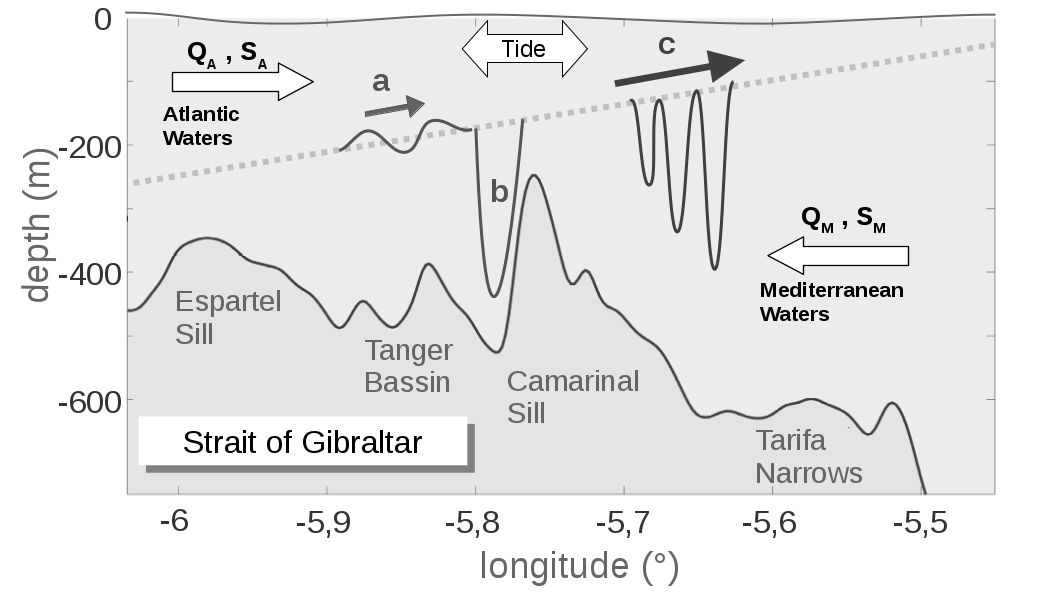
\includegraphics[width=0.51\textwidth]{./papier2D/schema_echange.png}
 \captionof{figure}{Mean exchange in the Strait of Gibraltar. The interaction of the tide with the stratification and bathymetry generates small-scale physical phenomenon. (a) Linear / Small amplitude internal wave. (b) Hydraulic Jump. (c) Large-amplitude internal waves or internal solitary waves (ISW).}
\label{scheme_GBR}
\end{wrapfigure}
%\end{figure}

Mass conservation leads indeed to : 
\begin{equation}  
	\label{Eq_mass}
    \displaystyle   
  	Q_A+Q_M = E-P
\end{equation}
and conservation of salt requires: 
\begin{equation}  
    \label{Eq_salt}
    \displaystyle   
    Q_A S_A + Q_M S_M =  0
\end{equation}
where $Q_A$ is the volume flux of Atlantic water (positive value), $Q_M$ is the volume flux of Mediterranean water (negative value) and $E-P$ is the space-averaged Evaporation minus Precipitation (and river runoff) water budget over the whole Mediterranean Sea. $E-P$ is positive. $S_A$ ($S_M$) stands for Atlantic (Mediterranean) water mean salinity and $S_M-S_A\approx 2\mbox{\textperthousand}$ (Bethoux, 1979). The excess of evaporation corresponds to a yearly averaged loss of water of about 1 meter (Garrett et al., 1990).\\

\textit{Dynamical control, maximum exchange and overmixed solution in the strait.}\\
The bathymetry of the region imposes a "dynamical control" (Baines, 1995) on the circulation in the Mediterranean basin. Such a control appears in regions of the ocean where the propagation of a particular type of waves is locally (temporally or continually) inhibited by large amplitude currents. This mechanism for the Strait of Gibraltar is illustrated in figure \ref{scheme_GBR}. In the strait, the control occurs when and where tides and water exchange generate currents with velocities larger than the velocities of the internal waves (denoted (a) in figure \ref{scheme_GBR}) propagating at the interface of Atlantic and Mediterranean waters. In the transition region a "hydraulic jump" can form (b).

Several more refined analytical models have been proposed to investigate the hydraulic control in the region of Gibraltar (Bryden and Stommel, 1984; Farmer and Armi, 1986 or Garrett et al., 1990). 
Traditionally, hydraulic controls may occur at Camarinal Sill (CS), Espartel Sill (ES), and Tarifa Narrows (TN), though the predicted location and time frequency of the appearances of these controls vary with the refinement of the model :
\begin{itemize}
\item{Farmer and Armi (1986)'s two-layer model takes into account the geometry of the strait (depth and breadth), the exchanged volumes ($Q_A$ and $Q_M$) and the salinity contrast ($S_A -S_M$). This simple model manages to predict the presence of two simultaneous hydraulic controls, one at the sill, the other at the contraction in TN, defining "maximal exchange regime"  (further details are given below). }

\item{In a slightly more elaborated model, the inclusion of the entrainment between the two layers and the subsequent introduction of a third interfacial layer modify the left-hand terms of equations (\ref{Eq_mass}) and (\ref{Eq_salt}) with the introduction of horizontal and vertical transports in this third layer (Bray, 1995). The critical conditions are also changed: new controls can in particular appear since there are now two interfaces, with potentially two baroclinic modes (Sannino et al., 2009).}

\item{ When now considering a three-dimensional flow, the definition of the control needs to integrate cross-strait variations such as the tilt of the interface in this direction (Sannino et al, 2009). In the maximal exchange solution, control in TN can for instance result in the detachment of the surface layer from the northern shore.}
\end{itemize}

These conditions on the flow, when combined with the above two conservation equations (\ref{Eq_mass}) and (\ref{Eq_salt}), can be used to relate volume fluxes and evaporation with the input salinity difference ($S_A-S_M$). As a consequence, local characteristics of the exchange flow in the Strait of Gibraltar can be linked to the formation of Mediterranean waters (Bryden and Stommel, 1984) and to the diapycnal mixing over the Mediterranean basin. The "overmixed solution" corresponds in this case to a minimal salinity difference and to a maximal exchange of mass.

In-situ observations suggest that this maximal exchange is attained only punctually in the strait during the year, the rest of the time the exchange is called "submaximal". Tidal currents impose a strong signature on this complex mechanism of hydraulic control in the strait at different timescales ranging from the tidal cycle to the neap/spring tidal modulation. Seasonal lower frequency can also change the occurrence and the locations of the hydraulic jumps.\\

\textit{Internal Solitary Waves.}\\
Those hydraulic jumps are large-amplitude depressions in the regions of hydraulic controls. There, intense mixing occurs between the Atlantic and Mediterranean waters, changing for example the characteristics of the Mediterranean outflow, which is one seasonal component of the circulation in the Northern Atlantic. 

The relaxation of those jumps generates large-amplitude, non-linear, non-hydrostatic trains of Internal Solitary Waves (ISW) (denoted (c) in figure \ref{scheme_GBR}). When the barotropic tide is constrained by the bathymetry of the strait, large vertical velocities appear and energy is transmitted to several normal modes of internal waves. In the Strait of Gibraltar, the largest amplitude ISW observed correspond to the first baroclinic mode (no change of direction of the induced velocity through the water column, all isopycnal surfaces are in phase). The signature of Modes 2 waves (vertical velocity profile showing one node, spreading of the isopycnals) has also been observed in the region of Gibraltar strait (Farmer and Armi, 1988, V\'azquez and al, 2006).

These waves propagate at the interface of Mediterranean and Atlantic water layers. In addition to their unknown impact on the local and remote mixing of the Atlantic and Mediterranean waters, the correct forecast of the generation and propagation of these peculiar waves still remains a challenge. \\

\textit{Consequences on basin-scale circulation.}\\
The region of the strait is thus relevant not only for its own dynamic and for the resulting peculiar turbulent cascade but also for its impact on both the outflowing Mediterranean and inflowing Atlantic waters. Indeed the various small-scale processes described above modify the characteristics of Atlantic and Mediterranean waters and, down the line, their behavior as they circulate respectively in the Mediterranean and in the Northern Atlantic.

To study these consequences in greater depth, numerical modeling is required. Some rudimentary models of the strait have for instance been achieved by modeling specifically the two layers of Atlantic and Mediterranean waters (Brandt 1996; Izquierdo 2001). With the increase in computational power, 3D modeling with greater vertical and horizontal sampling are feasible (Sannino et al., 2004). The tidal cycle and some features of the flow can be simulated. Several non-hydrostatic models have then been proposed (Sanchez Garrido, 2011; Sannino, 2014), which allows the representation of ISW. Other configurations include the strait of Gibraltar into a Mediterranean circulation model (Soto Navarro et al., 2014). Enhanced resolution in the strait (Naranjo et al., 2015) or nesting of a high-resolution grid of the strait in a lower-resolution model of the Mediterranean (Sannino et al., 2009) impact the stratification in the Mediterranean and improve the representation of convective events in the Gulf of Lion.\\
Lately, a new non-hydrostatic regional ocean model has been proposed (Auclair et al., 2018). It is based on regional ocean models (Symphonie in a research, Leap-Frog, 3-mode version and lately ROMS-CROCO in an efficient, LF-AM3, 2-mode version) in which the incompressible (Boussinesq-flow) assumption is relaxed together with the hydrostatic assumption. This new model opens new perspectives in terms of modeling of small-scale processes since Navier-Stokes equations can be simulated with much less restrictive numerical assumptions whereas computing costs have been drastically reduced following Shchepetkin and McWilliams (2005) advanced numerical technics.\\

% \\
%\textit{\textbf{What are the objectives of the present study ?}} \\

\textit{Objectives of the present study.}\\
The objectives of the present study are both numerical and physical. We show that a new generation of non-hydrostatic ocean models can be used to forecast complex non-linear, non-hydrostatic physics in a realistic, easy-to-implement and computationally-affordable configuration. The complete set of Navier-Stokes equations is integrated in time and it is presented for the very first time in such a complex region as Gibraltar.\\
The now-classical but still numerically-demanding chosen configuration is based on a lock-exchange initialization (Sannino et al., 2002). To the author knowledge, the present configuration can also be viewed as one of the very first (M)ILES\footnote{Monotonic implicit large eddy simulation \color{black}} model (Grinstein et al., 2007) of the region of Gibraltar. 
A 2D vertical subsection of the strait has been chosen in order to reduce the number of parameters having an impact on the studied dynamics. As such, the vertical subsection appears as an exploratory study preparing the implementation of a more complex fully 3D model in the studied region. In an obvious way, a 2D-vertical subsection is implemented firstly to reduce the computational cost and implementation burden. This leads us to propose an easy-to-implement and computationally-affordable tool that can be run in various contexts.\\

%\color{blue} A partir de là, il faudrait indiquer les subsections dans lesquelles sont détaillés les points cités (et au besoin la réorganiser un peu dans l'ordre chronologique. \color{black}.\\

In subsection 2 we give a review of the CROCO-NBQ model dynamics and we present the implementation of the 2D lock-exchange experiment. We carefully discuss and evaluate the way the bathymetry profile, the water masses, the exchange and tidal flows can be integrated in a forecasting system. In subsection 3 we evaluate the physics of the 2D configuration. In subsubsection 3.1 we compare the forecasted dynamics to published data such as in Farmer and Armi (1988), with emphasis on hydraulic controls, hydraulic jumps and mode-1 and mode-2 ISW (non-linear internal trains of solitary wave) propgation. The dispersion and damping of the train of mode 1 solitons as it propagates over the deeper eastern side of the strait is studied in subsubsection 3.2. To this aim, we compare the forecast with the Extended Korteweg-de Vries (eKdV) equation and with satellite images. Finally, both physical (topography, tidal amplitude) and numerical (spatial resolution, non-hydrostatic algorithm) sensitivity-tests are carried out respectively in subsections \ref{TestPhy} and \ref{TestNum}, with a focus on the changes on the fine-scales dynamics listed in figure \ref{scheme_GBR}.

%We investigate the dynamics of hydraulic jumps in areas of hydraulic controls. Modes 1 and 2 of non-linear internal trains of solitary wave are carefully studied and their forecast is compared to published data from Gibraltar Experiment (Army and Farmer, 1988). The region and date of generation and propagation of both modes are more particularly addressed. The propagation of the train of Mode-1 solitons over the deeper eastern side of the strait is then studied.

%Both numerical and physical sensitivity-tests are finally carried out. The advection of internal modes by the tidal current is also discussed. The dispersion and damping of the train of solitons are discussed and the model is compared with the Modified Korteweg-de Vries (KdV) equation and with satellite images.
% Based on this realistic configuration the forecasting capabilities of the model are finally more specifically evaluated.\\
% \\
% \textit{\textbf{Why did we choose a numerical configuration based on a 2D vertical subsection with a yet fully 3D ocean-model?}}


%We however have to make sure that the physics of the 2D subsection remains realistic and that the restriction to a  vertical subsection does not lead to specific unrealistic mechanisms.

%%%%%%%%%%%%%%%%%%%%%%%%%%%%%%%%%%%%%%%%%%%%%%%%%%%%%%%%%%%%%%%%%%%%%%%%%%%%%
\subsection{Numerical configuration}
%%%%%%%%%%%%%%%%%%%%%%%%%%%%%%%%%%%%%%%%%%%%%%%%%%%%%%%%%%%%%%%%%%%%%%%%%%%%%

%----------------------------------------------------------------------------
\paragraph{The numerical forecasting system}
%----------------------------------------------------------------------------

%\indent In the region of Gibraltar, the Atlantic inflow and Mediterranean outflow circulations and the barotropic tidal waves interact with the narrow and shallow (less than 1 km deep) topography of the strait. Hydraulic jumps, non-linear internal waves, small-scale shear instabilities... are generated in the region of the strait leading to very energetic fine scale dynamics. \color{blue} L'introduction de cette partie est peu longue car tu as déjà traité tout cela dans la subsection précédente. \color{black}.

The proposed numerical model of the Strait of Gibraltar simulates explicitly the fine-scale processes (from tens to hundreds of meters) discussed previously. This means that (i) a sufficient grid resolution must be provided in the strait and (ii) a dedicated numerical kernel must be used.

The non-hydrostatic (non-Boussinesq) version of the CROCO community ocean model (CROCO- NBQ) is thus chosen for his ability to allow LES\footnote{LES (Large Eddy Simulation): LES, in contrast to DNS (Direct Numerical Simulation) does not simulate the full 3D Kolmokorov-like energy cascade down to molecular scales. However at least the onset of this cascade is explicitly represented unlike in RANS (Reynolds Averaged Navier-Stokes).} and it is implemented in a realistic configuration in order to evaluate its capacity to forecast complex non-hydrostatic dynamics in an easy-to-implement configuration. In LES, the direct transfer ends at the lowest scale resolved, and subgrid dissipation of energy is accomplished by implicit mixing of the advective scheme, as well as by explicit parametrisation.

The regional ocean model CROCO-NBQ is an extension of ROMS from which it inherited the robustness and efficiency of the time-splitting (Shchepetkin and McWilliams, 2005 , Debreu et al, 2012). CROCO-NBQ is based on a time-splitting algorithm: the numerics of the "slow" mode is similar as ROMS internal mode (Shchepetkin and McWilliams, 2005) whereas the "fast mode" has lately been adapted to include both the "External mode" and the evolution of the s-grid of ROMS-AGRIF together with an evolution of the non-hydrostatic and non-Boussinesq kernel of Symphony-NBQ model (Auclair et al., 2018). A two-mode time-splitting kernel is conserved but if the slower, internal mode, is only slightly modified by introducing a prognostic calculus of vertical momentum, the fast mode (once barotropic) now deals with a 3D-compressible flow. \\

 %----------------------------------------------------------------------------
 \paragraph{Continuous free-surface compressible equations in z-coordinates}
 \label{NavierStokes}
 %----------------------------------------------------------------------------
 
\indent The full set of Navier-Stokes equations for a free-surface ocean is explicitly integrated and the continuity and momentum equations, the surface kinematic relation, the heat, salt and state equations respectively read in Cartesian coordinates: 
\begin{alignat}{2}
  \displaystyle
   %%%%%%%%%%%%%%%%%%%%%%%%%%%%%%%%%%%%%%%%%%%%%%
   % Continuity
   %%%%%%%%%%%%%%%%%%%%%%%%%%%%%%%%%%%%%%%%%%%%%%
   &\partial_t\rho &&=-\vec{\nabla}.(\rho\vec{v})\\[3mm]
   %%%%%%%%%%%%%%%%%%%%%%%%%%%%%%%%%%%%%%%%%%%%%%
   % Momentum
   %%%%%%%%%%%%%%%%%%%%%%%%%%%%%%%%%%%%%%%%%%%%%%
   \label{momentum}
   &\partial_t\rho\vec{v} &&=
   -\vec{\nabla}.\left(\rho\vec{v}\otimes\vec{v}\right)
   -2\rho\vec{\Omega}\wedge\vec{v}
   -\vec\nabla p+\rho\vec{g}
   +\mu\Delta\vec{v}
   +\lambda\vec{\nabla}(\vec{\nabla}.\vec{v})\\[3mm]
   %%%%%%%%%%%%%%%%%%%%%%%%%%%%%%%%%%%%%%%%%%%%%%
   % Surface kinematic relation
   %%%%%%%%%%%%%%%%%%%%%%%%%%%%%%%%%%%%%%%%%%%%%%
   &\partial_t{\zeta} &&= 
   w\scriptstyle(z=\zeta)\textstyle
   -\vec{v}\scriptstyle(z=\zeta)\textstyle.\vec{\nabla}{\zeta}\\[3mm]
   %%%%%%%%%%%%%%%%%%%%%%%%%%%%%%%%%%%%%%%%%%%%%%
   % Heat equation
   %%%%%%%%%%%%%%%%%%%%%%%%%%%%%%%%%%%%%%%%%%%%%%
   &\partial_t{\rho\theta} &&=-\vec{\nabla}.\left(\rho\theta\vec{v}\right)
   +\kappa_{\theta}\Delta\theta\\[3mm]
   %%%%%%%%%%%%%%%%%%%%%%%%%%%%%%%%%%%%%%%%%%%%%%
   % Salt equation
   %%%%%%%%%%%%%%%%%%%%%%%%%%%%%%%%%%%%%%%%%%%%%%
   &\partial_t{\rho s} &&=-\vec{\nabla}.\left(\rho s\vec{v}\right)
   +\kappa_{s}\Delta s\\[3mm]
   %%%%%%%%%%%%%%%%%%%%%%%%%%%%%%%%%%%%%%%%%%%%%%
   % State equation
   %%%%%%%%%%%%%%%%%%%%%%%%%%%%%%%%%%%%%%%%%%%%%%
   &\rho &&=\varrho\left(\theta,s,P\right)
\end{alignat}
where $\vec{v}=(u,v,w)$ is the velocity, $p$ the total pressure, $\zeta$ the free-surface anomaly $\rho$ the density, $\theta$ and s respectively the potential temperature and salinity. $\vec{\Omega}$ is the instantaneous earth rotation vector, $\vec{g}$ is the acceleration of gravity and $\mu$, $\lambda$, $\kappa_{\theta}$ and $\kappa_{s}$ are respectively the dynamical and second (bulk) viscosity and the thermal and salinity diffusivities.

   
 %----------------------------------------------------------------------------  
 \paragraph{Density and pressure decomposition}
 %----------------------------------------------------------------------------
\indent To allow ROMS-like time-splitting, density is decomposed into slow and fast components based on a first-order decomposition with respect to total pressure. In the following, s and f subscripts respectively refer to slow and fast-mode components.\\
\begin{alignat}{2}
  \displaystyle
   %%%%%%%%%%%%%%%%%%%%%%%%%%%%%%%%%%%%%%%%%%%%%%
   % Density
   %%%%%%%%%%%%%%%%%%%%%%%%%%%%%%%%%%%%%%%%%%%%%%
  &\rho &&=\rho_{s}\left(\theta,s,P\right)
  +\overbrace{\left.{\frac{\partial{\rho}}{\partial{P}}}\right|_{\theta,s}\delta{P}}^{\delta{\rho}=\rho_{f}}
  +O\left(\delta{P}^2\right)\\
   %%%%%%%%%%%%%%%%%%%%%%%%%%%%%%%%%%%%%%%%%%%%%%
   % Pressure
   %%%%%%%%%%%%%%%%%%%%%%%%%%%%%%%%%%%%%%%%%%%%%%
  &P &&=\underbrace{P_{atm}
  +\int\limits_z^{\zeta}{(\rho_{s}-\rho_0)g\ dz'}}_{Slow\ mode}
  +\underbrace{\rho_{0}g(\zeta-z)+\underbrace{\delta P}_{P_{f}}}_{Fast\ mode}
\end{alignat}
  
No further decomposition is required for other variables.
  
 
%----------------------------------------------------------------------------  
 \paragraph{Slow vs fast components}
 %----------------------------------------------------------------------------
\indent Navier-Stokes equations are consequently integrated with two different time-steps in a time-splitting algorithm. The slow mode is identical to ROMS slow "internal" mode whereas the fast-mode (unlike in ROMS) is 3D and allows the integration of the compressible terms of the momentum and continuity equations and of the free-surface anomaly through the free-surface kinematic condition.
\begin{equation}
  \begin{split}
  %\begin{equation}
    \displaystyle
   %%%%%%%%%%%%%%%%%%%%%%%%%%%%%%%%%%%%%%%%%%%%%%
   % Continuity
   %%%%%%%%%%%%%%%%%%%%%%%%%%%%%%%%%%%%%%%%%%%%%%
   &\partial_t\ \rho_f &= -\partial_t\ \rho_{s}
   &-\vec{\nabla}.(\rho\vec{v})\\
   %%%%%%%%%%%%%%%%%%%%%%%%%%%%%%%%%%%%%%%%%%%%%%
   % Momentum
   %%%%%%%%%%%%%%%%%%%%%%%%%%%%%%%%%%%%%%%%%%%%%%
   &\partial_t\rho\vec{v} &= 
   & \overbrace{-\vec{\nabla}.\left(\rho\vec{v}\otimes\vec{v}\right)
   -2\rho\vec{\Omega}\wedge\vec{v}
   -\vec\nabla(\int\limits_z^{\zeta_f}{(\rho_{s}-\rho_0)g\ dz'})
   +\mu\Delta\vec{v}}^{\vec{\Lambda}_{s}}\\
   & & &\underbrace{-\rho_{0}g\vec\nabla\zeta_f
   -\vec\nabla{P}
   +\rho\vec{g}
   +\lambda\vec{\nabla}(\vec{\nabla}.\vec{v})}_{\vec{\Lambda}_{f}}\\
   %%%%%%%%%%%%%%%%%%%%%%%%%%%%%%%%%%%%%%%%%%%%%%
   % Surface kinematic relation
   %%%%%%%%%%%%%%%%%%%%%%%%%%%%%%%%%%%%%%%%%%%%%%
.   &\partial_t{\zeta_f} &&= 
   w_f\scriptstyle(z=\zeta)\textstyle
   -\vec{v_f}\scriptstyle(z=\zeta)\textstyle.\vec{\nabla}{\zeta_f}\\[3mm]
   %%%%%%%%%%%%%%%%%%%%%%%%%%%%%%%%%%%%%%%%%%%%%%
   % Heat equation
   %%%%%%%%%%%%%%%%%%%%%%%%%%%%%%%%%%%%%%%%%%%%%%
   &\partial_t{\rho\theta_s} &=\ &\Theta_{s}=-\vec{\nabla}.\left(\rho\theta_s\vec{v}\right)
   +\kappa_{\theta}\Delta\theta_s\\
   %%%%%%%%%%%%%%%%%%%%%%%%%%%%%%%%%%%%%%%%%%%%%%
   % Salt equation
   %%%%%%%%%%%%%%%%%%%%%%%%%%%%%%%%%%%%%%%%%%%%%%
   &\partial_t{\rho s_s} &= &\ S_{s}= -\vec{\nabla}.(\rho s_s\vec{v})
   +\kappa_{s}\Delta{s_s}\\
   %%%%%%%%%%%%%%%%%%%%%%%%%%%%%%%%%%%%%%%%%%%%%%
   %State equations
   %%%%%%%%%%%%%%%%%%%%%%%%%%%%%%%%%%%%%%%%%%%%%%
   &\rho_s &= &\varrho(\theta_s,s_s,\zeta_f)\\
   &\rho_f &= &c_s^{-2} P_f
  \end{split}
\end{equation}
  
No indice is specified for momentum since this variable is integrated both in slow and fast modes. Slow (fast) prognostic equations and diagnostic relations are respectively integrated in slow (fast) mode. Momentum equations are integrated in both modes. More details can be found in Auclair et al. (2018).

%----------------------------------------------------------------------------  
 \paragraph{Bathymetry of the numerical configuration}
 \label{BathyNum}
 %----------------------------------------------------------------------------
%%%%%%%%%%%%
% Figure 1
%%%%%%%%%%%%
\begin{figure}[!h]
\centering
 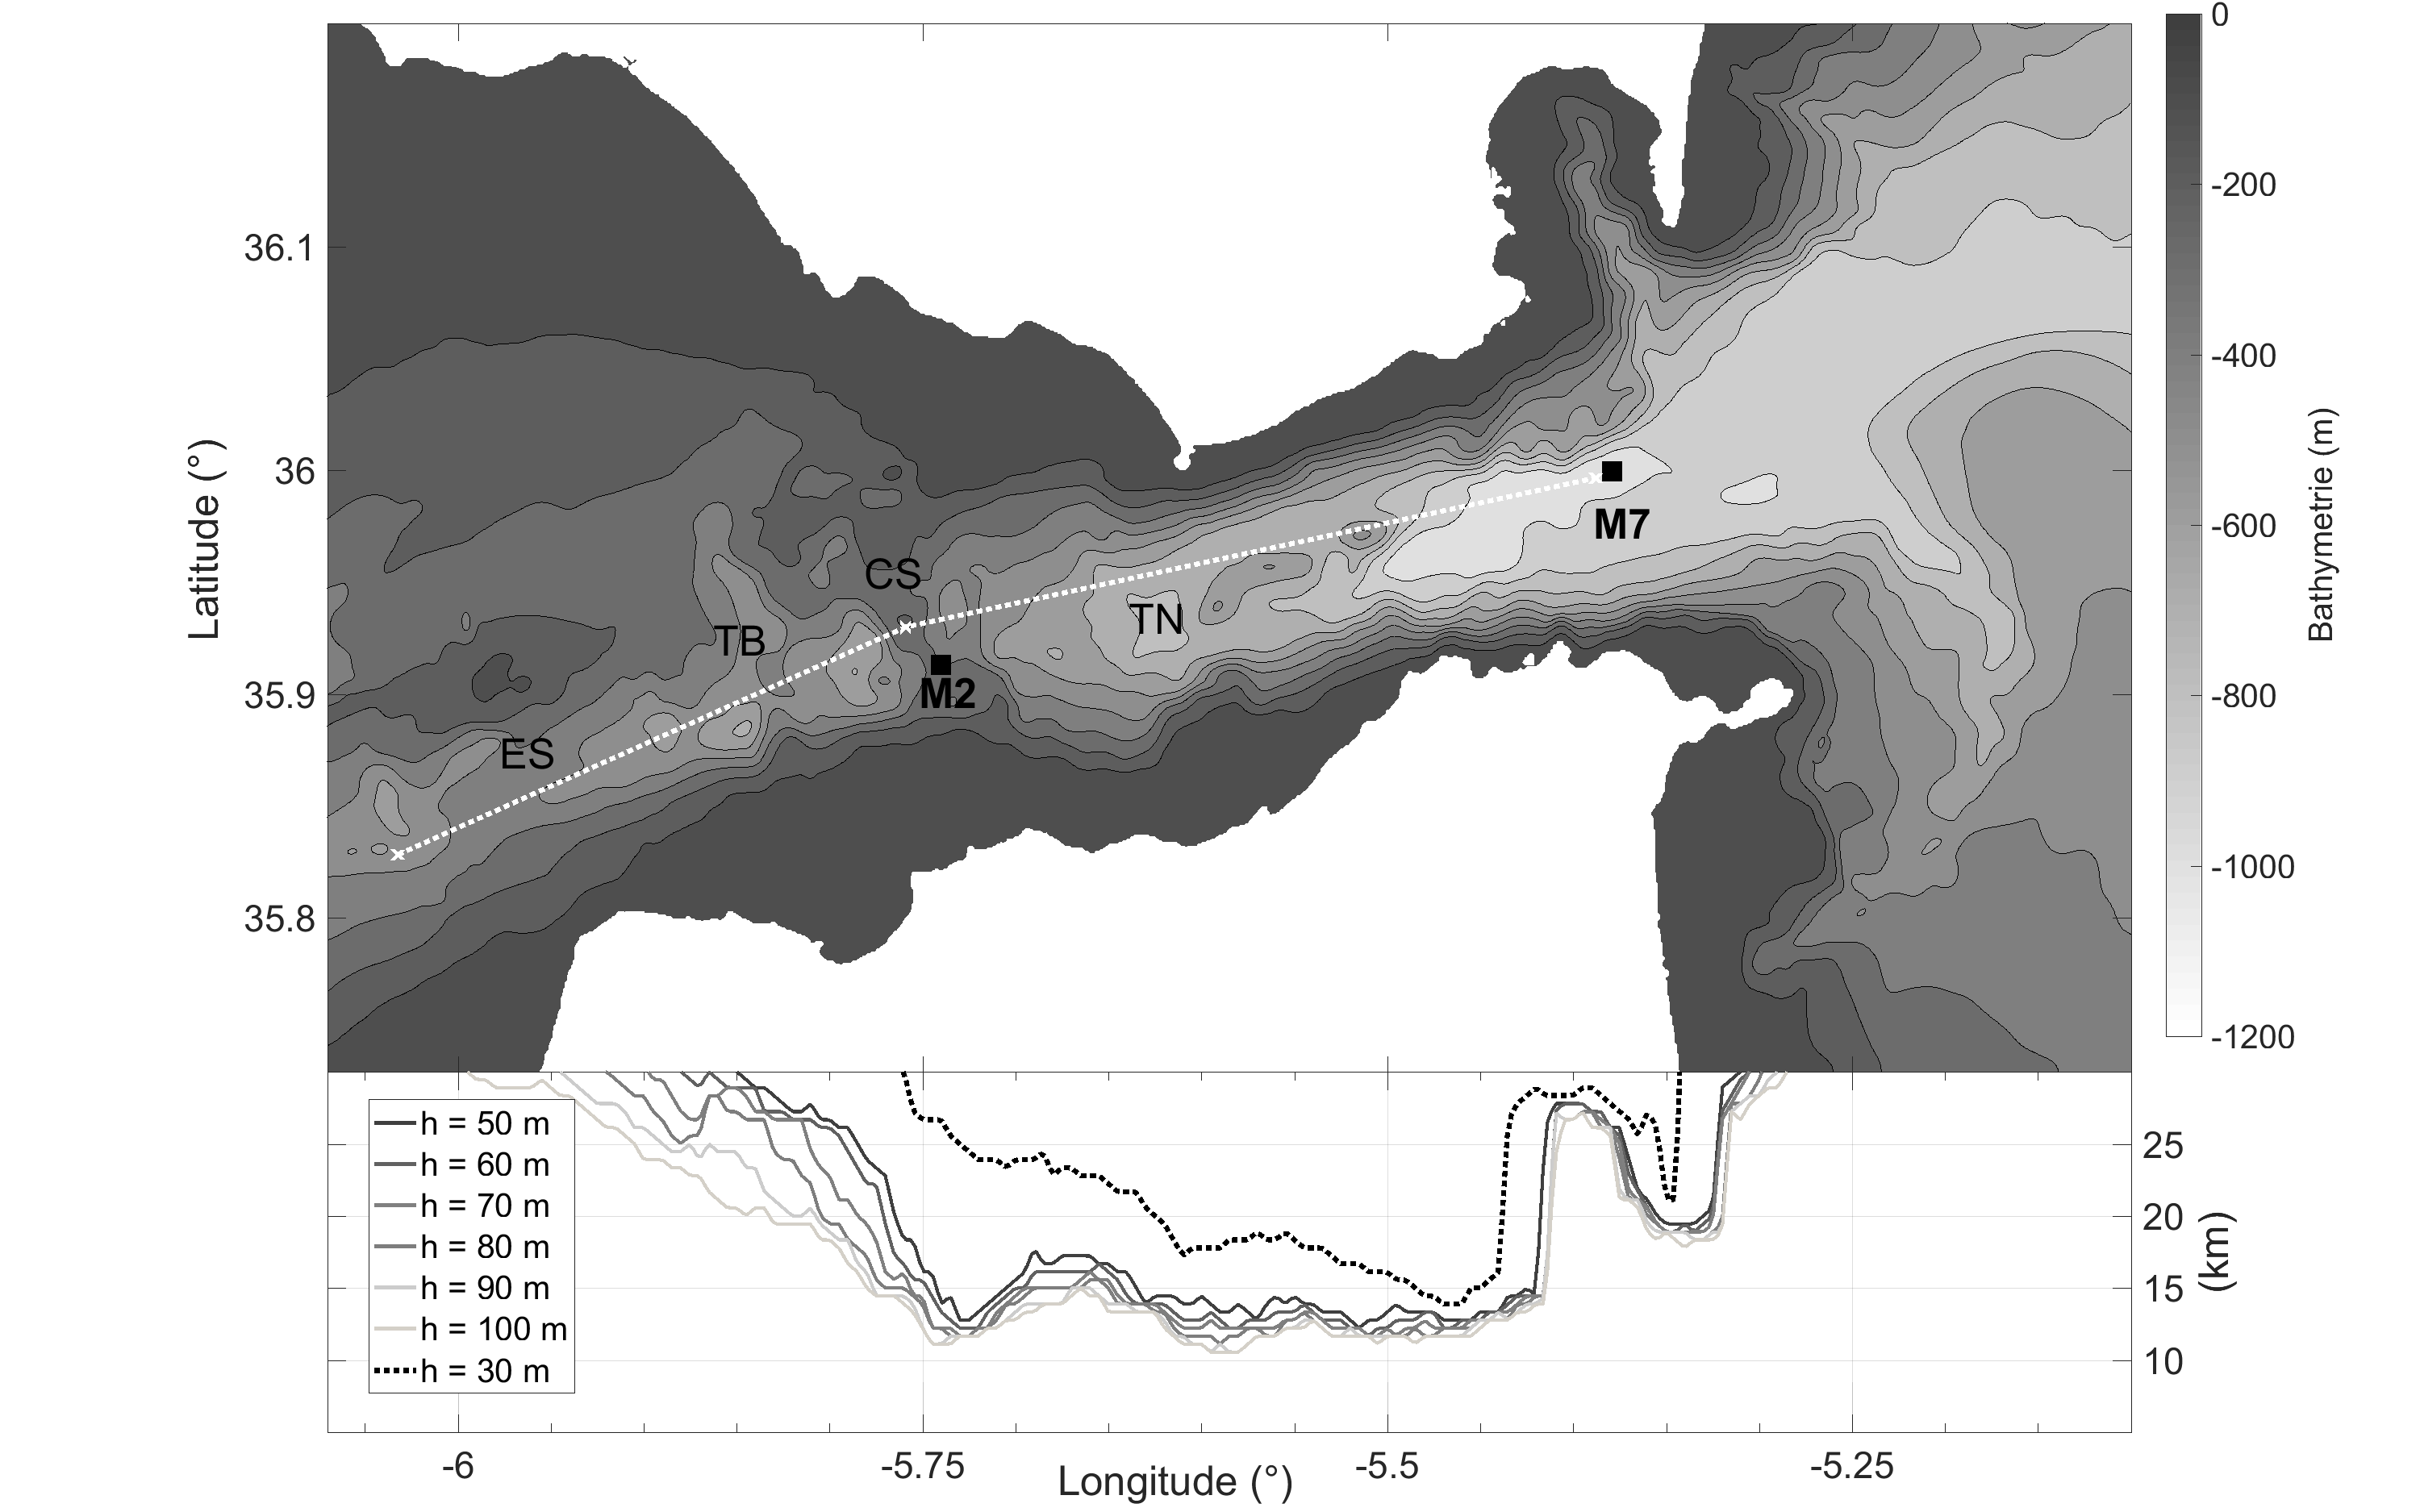
\includegraphics[width=1\textwidth]{./papier2D/bathy3d+Rr3d.png}
 \caption { a) Bathymetry of the strait of Gibraltar, location of the transect A (white dotted line). Black squares indicate the position of moorings. (ES: Espartell Sill, TB: Tanger Basin, CS: Camarinal Sill , TN: Tarifa Narrows)
 b) Maximum distance along the transverse (y) direction between 2 isobaths of depth h.}
 \label{Fig1}
\end{figure}

\indent In figure \ref{Fig1}.a is depicted the 500 m-resolution bathymetry developped in the framework of the HOMONIM project coordinated by the French Navy (SHOM) and MeteoFrance as provided by the French Navy, with the  principal geographical features as well as the localization of the studied vertical 2D subsection. This subsection is chosen as close as possible to the transect of Farmer and Armi's Gibraltar Experiment realized in April 1986 (Farmer and Armi, 1988). Hereafter, $u$ is defined as the velocity in the longitudinal direction and $v$ the velocity in the transverse direction. Figure \ref{Fig1}.b presents the width of the Strait of Gibraltar relative to different reference depths. This plot indicates that an averaged strait width of approximately 13 km can be chosen, evidencing the steep slopes at the lateral boundaries of the straits, especially in Tarifa Narrows.

Simulations are successively achieved with horizontal resolutions of 220 m and then 50 m. So as to limit the unrealistic effect of punctual seamounts in the transverse direction such as those found in TN (which can, in a vertical 2D subsection, end up acting as another sill), a Gaussian interpolation of the bathymetry is provided with a greater Gaussian radius in the transverse direction than in the longitudinal direction. In the following, the Gaussian radius in the transverse direction is chosen equal to 1500 m (ie. inferior to the width of the strait in figure \ref{Fig1}.b). As a consequence, the bathymetry only reflects the deepest areas in the canal. 
%corresponds approximately to half the width of the 1000-m deep canal in the region of TN. 
In the longitudinal direction, the Gaussian interpolation radius is only 300 m to preserve bathymetry variability in this direction.

Using this method to interpolate bathymetry, the minimum depth at Camarinal Sill, the main sill of the Strait of Gibraltar, goes from the real value of approximately 200 m to 247.6 m. Further characteristics of the reference forecast based on this bathymetry (hereafter named \textbf{SimRef}) are presented in table \ref{tabsimref}.\\

%--------------------------------
\paragraph{Water mass and tidal forcing}
%--------------------------------
\indent Realistic forecasts of limited-area domains require at least temperature and salinity profiles in the studied region and, as a consequence, they are not easy to initialize nor to constrain at their open boundaries. A minimum number of two profiles is needed to initialize gradients associated to sloping isopycnal surfaces in a given direction. Following Sannino et al. (2002), a lock-exchange initialization of the region of the strait can be implemented with Atlantic water on the western side of CS and Mediterranean water on the eastern side at t = 0 s. A three-day period of simulation (spin-up phase) is then achieved to set up the exchange flow in the strait.

The initial temperature and salinity profiles are presented in figure \ref{fig_LEx}, where we see a contrast in salinity between Atlantic and Mediterranean water, with respective mean of 35.9 and 38.2. In the following, the interface between the Atlantic and Mediterranean layers in terms of salinity is chosen as the 37 isohaline (Bryden, 1994). Density is now expressed as an anomaly (written $\rho'$) relative to a reference density $\rho_{0}$ computed by the model. In the following, if not specifically specified,the reference density is $\rho_{0}=1033.7$ kg/m$^3$.

The M2 tidal forcing (of period T = 12.4 h) is activated only after the spin-up period. It is simulated by a barotropic current of amplitude 0.4 m/s at the western boundary (0.8 m/s at CS). This corresponds to a neap-tide regime in the TPXO-8 tidal atlas (Egbert and Erofeeva, 2002).

\vspace{1\baselineskip}
\begin{minipage}{.4\textwidth}
%\begin{table}
\centering
\begin{tabular}{|p{\linewidth/3}|c|c|}
\hline
Number of horizontal points & \multicolumn{2}{c|} {602x3}  \\
%\hline
$\Delta x$ & \multicolumn{2}{c|} {221 m}\\ 
%\hline
Number of $\sigma$-levels & \multicolumn{2}{c|} {40} \\
%\hline
Depth & Min & Max\\
%\cline{2-3}
   & 247.6 m & 900 m\\
%   \hline
   $\Delta$z & 6 m & 23 m\\
%\hline
$\Delta t_s$ & \multicolumn{2}{c|} {4 s}\\
%\hline
$\Delta t_f$ & \multicolumn{2}{c|} {0.5 s}\\
%\hline
Vertical Viscosity & \multicolumn{2}{c|} {$10^{-6}$ m$^2$/s}\\
%\hline
Lateral Viscosity & \multicolumn{2}{c|} {$10^{-5}$ m$^2$/s}\\
%\hline
Diffusivity & \multicolumn{2}{c|} {$10^{-6}$ m$^2$/s}\\
%\hline
Momentum Advective Scheme & \multicolumn{2}{c|} {TVD}  \\
%\hline
TS Advective Scheme & \multicolumn{2}{c|} {WENO5}  \\
\hline
\end{tabular}
\captionof{table}{Numerical parameters of simulation \textbf{SimRef}}
\label{tabsimref}
\end{minipage}
%\end{table}
 ~
\begin{minipage}{.4\textwidth}\centering
%\begin{figure}[!t]
 \centering
 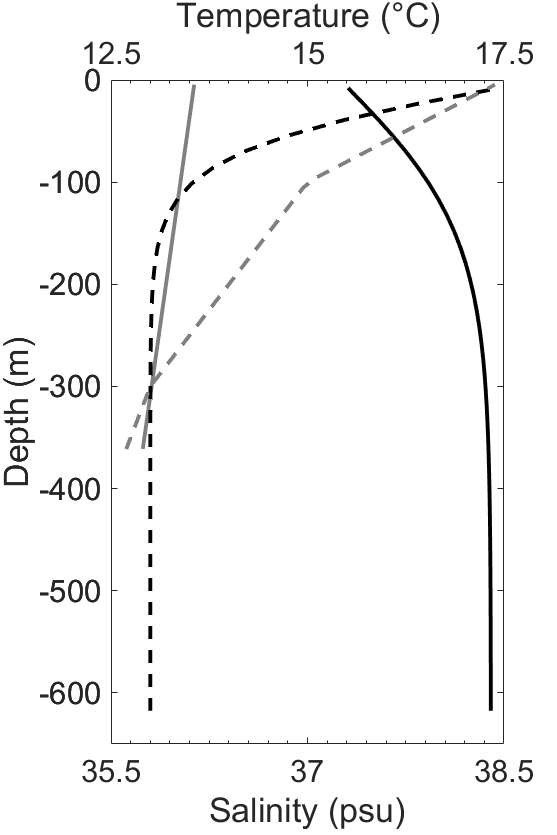
\includegraphics[width=\linewidth]{./papier2D/profil_LEx.png}
 \captionof{figure} {Salinity and temperature (dashed lines) profile of Mediterranean water (red) and Atlantic water (blue) at initial time-step}
\label{fig_LEx}
%\end{figure}
\end{minipage}
\vspace{1\baselineskip}



% ~
%%\begin{minipage}{.6\textwidth}\centering
%\begin{figure}[!t]
% \centering
% 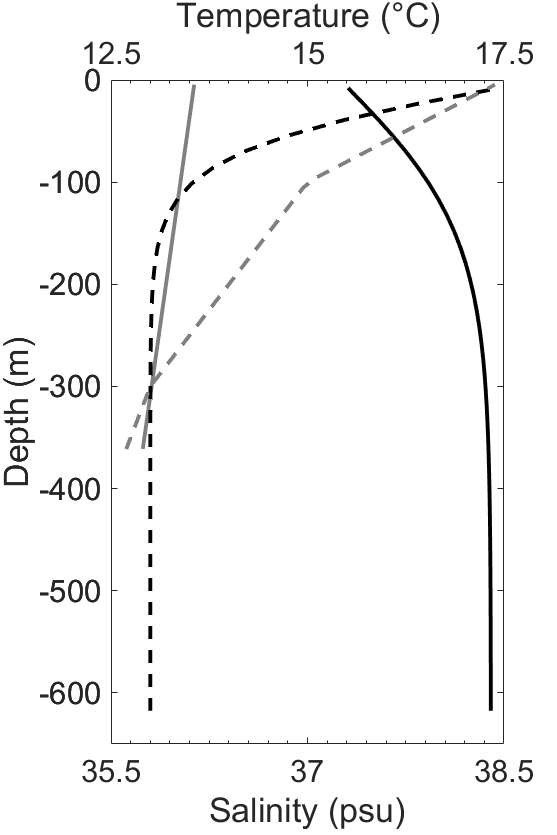
\includegraphics[width=0.6\textwidth]{./papier2D/profil_LEx.png}
% \captionof{figure} {Salinity and temperature (dashed lines) profile of Mediterranean water (black) and Atlantic water (grey) at initial time-step}
%\label{fig_LEx}
%\end{figure}
%%\end{minipage}


 
%----------------------------------------------------------------------------
\paragraph{Initialization of density profile and shear current : effect of Coriolis Pseudo-Force}
\label{Coriolis}
%----------------------------------------------------------------------------

The lateral boundaries of the strait of Gibraltar are distant of about 15 km, with a clear funneling effect from CS to the end of the strait when looking at subsurface isobaths (see figure \ref{Fig1}.b). The internal Rossby radius $R={\sqrt{g'h}}/{f}$ is usually observed as varying between 10 and 20 km (Bormans and Garrett 1989, Candela 1990, Vlasenko and al 2009). Here $g'= g (\rho_M(S_M) - \rho_A(S_A))/\rho_0$ is the reduced gravity, $h=h_1 h_2/(h_1+h_2)$ is a characteristic height with $h_1$ and $h_2$ respectively the upper and lower layer thicknesses, and $f$ is the Coriolis parameter. The width of the strait and $R$ are of the same order, indicating that rotational effects due for instance to geostrophy can be neglected as a first approximation. 

Hence, the balance is mainly between acceleration and the pressure force in equation (\ref{momentum}) and geostrophic adjustment in the along-strait direction is locally neglected. In observations (Farmer and Armi, 1988) and 3D-modeling configuration (Saninno, 2002), the consequences of Earth's rotation are a cross-strait shear of along-strait velocity (Bormans and Garett, 1989) and a tilt of the interface between Mediterranean and Atlantic waters, with greater velocities and a deeper interface along the southern (Moroccan) coast.

%
%%%%%%%%%%%%
% Figure 
%%%%%%%%%%%%
\begin{figure}[!t]
 \centering
 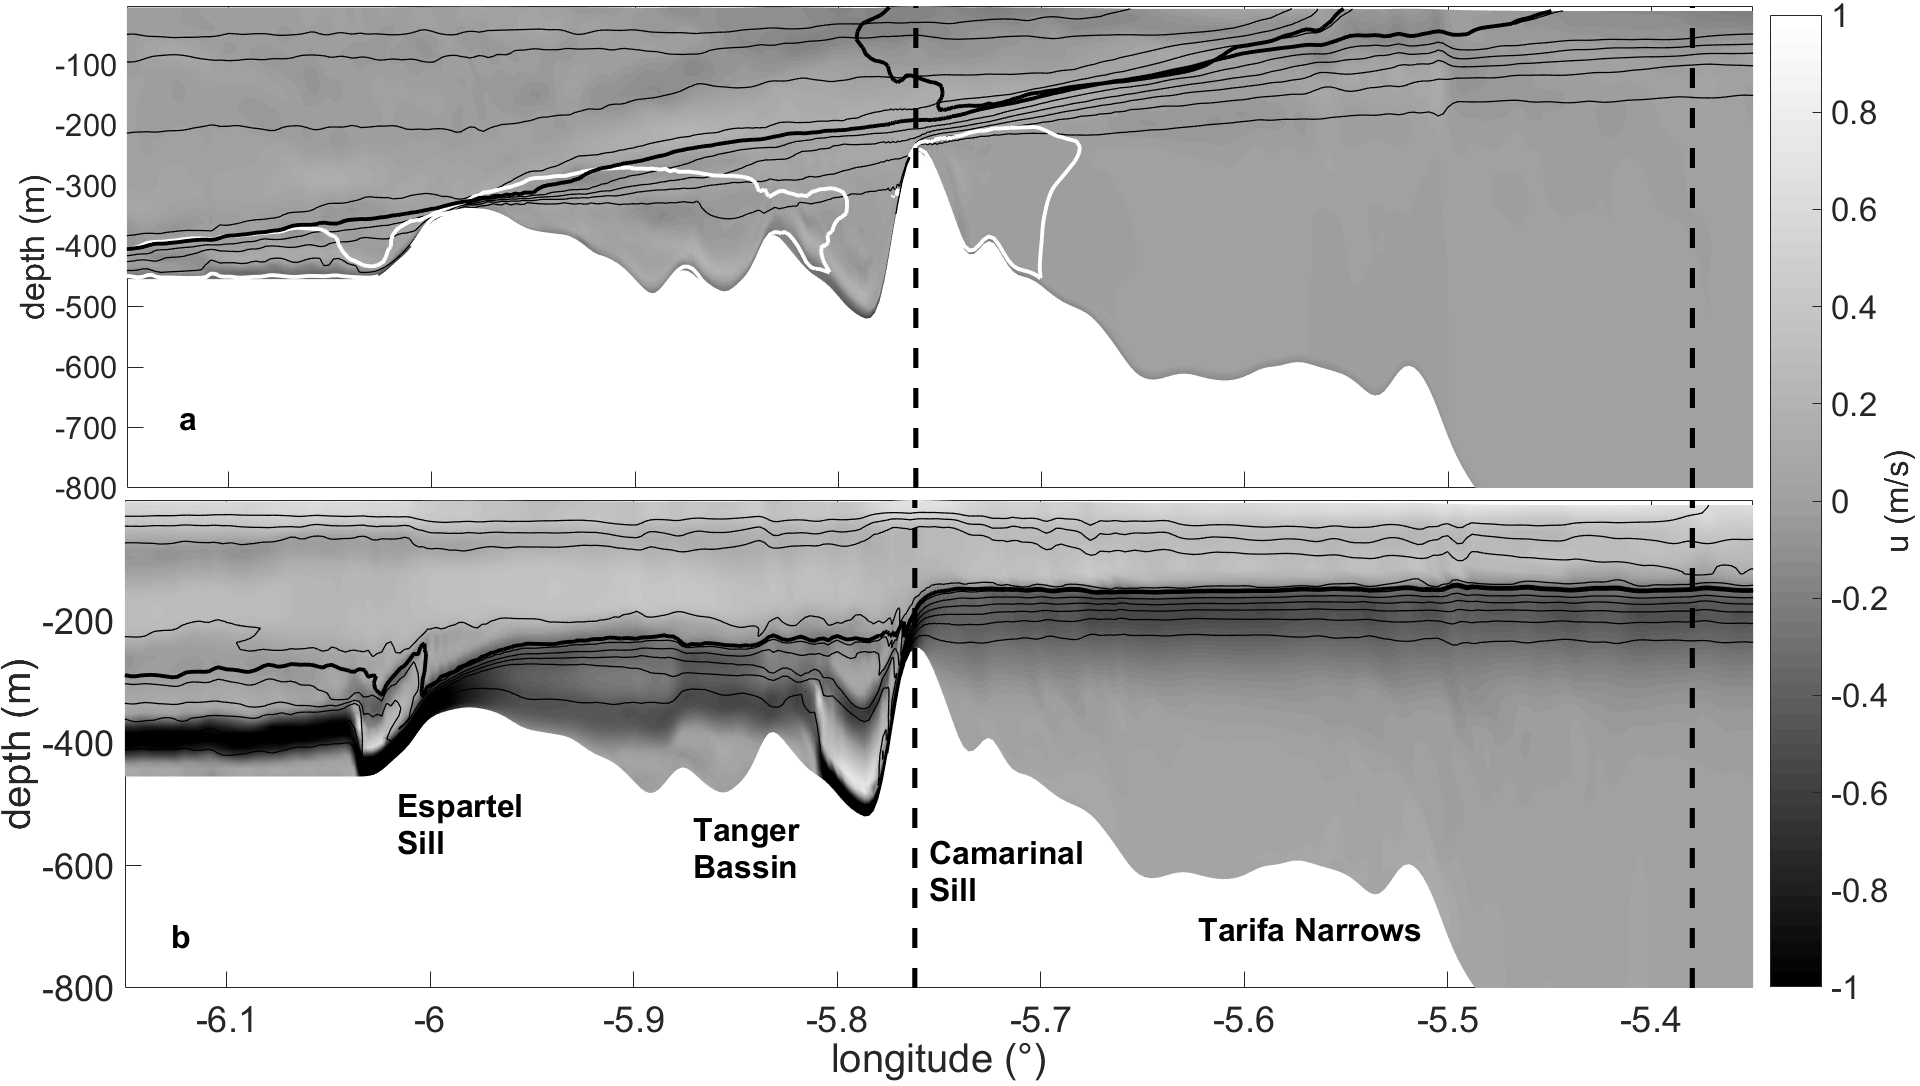
\includegraphics[width=1\textwidth]{./papier2D/stratif_corio_vs_nocorio.png}
 \caption {Longitudinal current and isopycnal contours at 70 h during the spin-up phase for \textbf{SimAllCor} (a) and \textbf{SimNoCor} (b).
 White contour : transversal current $v = 0.5 \ m/s$  Black contour : transversal current v=-0.5 \ m/s. Bolded isopycnal $\rho' = -0.7 \ kg/m^3$.
 The vertical dashed lines indicate the location of the profiles given in figure \ref{fig_current}.}
  \label{fig2}
\end{figure}
The transverse flow, the lateral boundaries and the resulting ``funeling effect'' cannot be simulated in a 2D vertical subsection, and we consequently need to examine how this limitation impacts both the stratification and the mean circulation. For this, we compare the initialization of a simulation with (i) the Coriolis pseudo-force activated from start to end (\textbf{SimAllCor}) ($f = 8.5 \ 10^{-5} s^{-1}$), (ii) a simulation without the Coriolis pseudo-force (the Coriolis parameter is set to zero) (\textbf{SimNoCor}), and (iii) a simulation with the Coriolis pseudo-force activated only after the spin-up period (\textbf{SimRef}). Apart from the choice of Coriolis parameter, the three simulated vertical subsections have the characteristics given in table \ref{tabsimref} for \textbf{SimRef}.

During the very first hours of simulations, the 'Lock-Exchange dam' separating the Atlantic and Mediterranean water-masses disappears, a gravity current is generated with dense Mediterranean waters flowing down the slope of CS and light Atlantic water spreading in the surface layer.
%\afterpage{
%%%%%%%%%%%
% Figure 
%%%%%%%%%%% 
%\begin{figure}[!t]
%\centering
%\includegraphics[width=\textwidth]{comp_UV_M.png}
%\caption {Mean zonal current (blue) and meridional current (red) above CS averaged over 3T at stations M2 and M7 for configurations %\textbf{SimAllCor} and \textbf{SimNoCor}(right). Locations of profile are given in Figure \ref{fig2}.}
%\label{fig_current}
%\end{figure} 


\begin{minipage}{0.45\textwidth}
%\begin{figure}
  \centering
  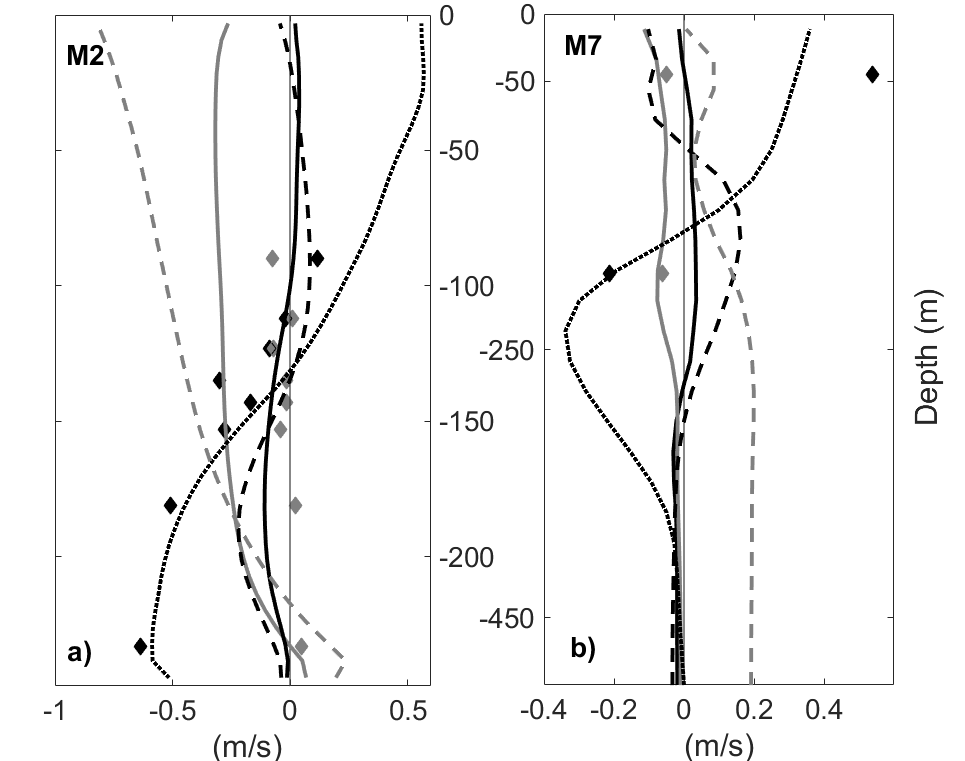
\includegraphics[width=\textwidth]{./papier2D/UV_CS_3T_ref.png}
  \captionof{figure}{3T-averaged longitudinal (black) and transversal current (grey) at the locations in figure \ref{fig2} for configurations \textbf{SimRef} (plain) \textbf{SimAllCor} (dashed) and \textbf{SimNoCor}(dotted). Tidally averaged measures of currents at stations M2 and M7 (figure \ref{Fig1}) in Candela et al. 1990 (diamonds).}
  \label{fig_current}
\end{minipage}
%\end{figure}
~
\begin{minipage}{0.45\textwidth}
%\begin{table}
\centering
\begin{tabular}{|c|m{0.22\linewidth}|m{0.22\linewidth}|}
\hline
& Upper layer transport & Lower layer transport\\
\hline
\textbf{SimAllCor} & 1.28 & -9.16\\
\hline
\textbf{SimNoCor} & 45.04 & -43.5 \\
\hline
\textbf{SimRef} & 0.7 & -6.43\\
\hline
\end{tabular}
\captionof{table}{3T averaged transports at CS (m$^2$/s)}
\label{tab_transport}
\end{minipage}
%\end{table}

%}%
%
\vspace{2\baselineskip}
 



Figure \ref{fig2} presents the field of longitudinal velocity ($u$) as well as some isopycnal contours for \textbf{SimAllCor} (a) and \textbf{SimNoCor} (b) at t = 70 h. The bolded isopycnal surface $\rho'= -0.7\ kg/m^3$ corresponds at that time to the 37 psu-isohaline. In figure \ref{fig2}.a are also plotted the transverse-velocity ($v$) isotachs $\pm$ 0.5 m/s. In the folowing figure \ \ref{fig_current} are plotted the averaged component of $u$ and $v$ in the water column at the two dashed vertical lines shown on figure \ref{fig2}. These locations correspond to moorings indicated in the figure \ref{Fig1} of Candela et al. (1990). Using the 37-psu isohaline as a frontier between the two water masses, the 3T time-averaged transport through the left dashed line at CS is calculated in table \ref{tab_transport}.

In \textbf{SimNoCor} configuration (Figure \ref{fig2}.b), a clear vertical shear of along-subsection velocity can be found between the two water masses. The shear is still featured in the 3T-averaged current profiles of figure \ref{fig_current}.b and is in accordance with the observations given by the moorings. The currents obtained in configurations \textbf{SimAllCor} and \textbf{SimRef} are weaker, with locally negative currents in the upper layer (see both figures \ref{fig2} and \ref{fig_current}). This is confirmed by the layer-averaged transports presented in figure \ref{fig_current}. Indeed, the amplitudes simulated in \textbf{SimAllCor} and \textbf{SimRef} are one order of magnitude smaller than in \textbf{SimNoCor}. 
 
In configurations \textbf{SimAllCor} and \textbf{SimRef}, the velocity in the cross-subsection direction is consequently due to the inclusion of the Coriolis pseudo-force. More precisely, during the spin-up phase of \textbf{SimAllCor}, the effect of rotation cannot be neglected anymore after only 6 hours. At that time, the upper Atlantic layer has spread over a distance of about 26 km and the cross-subsection velocity featured in figure \ref{fig2}.a is already present.

Without the lateral boundaries of the strait to inhibit geostrophic adjustment, the initially along-subsection gravity current is then almost completely converted into transverse geostrophic currents with spurious (non physical) consequences on the slope of the isopycnal surfaces. Indeed, geostrophy enables a thermal-wind balance for the transverse (v) component following: 
\begin{equation}  
    \label{Thermal_wind}
    \displaystyle   
	\frac{\partial v}{\partial z}
    =-\frac{g}{\rho_0 f} \frac{\partial \rho}{\partial x}
\end{equation}
This is particulary apparent in the east of CS in figure \ref{fig2}.a where the pycnocline is located at the transition between positive and negative transverse velocities (v). As a result, the pycnocline slope is $\Delta z/\Delta x = 6.10^{-3}$ (table \ref{tabdepth}) and the Atlantic water cannot spread further than the resulting surface front.

In \textbf{SimRef}, the Coriolis pseudo-force does not vanish. The initial state is presented in figure \ref{fig2}.b. Hence, the resulting slope and transverse velocity are smaller than in \textbf{SimAllCor}% (figure \ref{fig_current}.c)
. The pycnocline in the eastern part of the domain is deeper whereas it is shallower in the western part. However, the along-subsection currents remain weak.

In contrast, in configuration \textbf{SimNoCor} no such balance is allowed and, away from the sills, $\Delta z/\Delta x$ vanishes. In the along-subsection direction, the main balance is between the pressure force $(-1/\rho_0\  \partial p/\partial x)$ and the acceleration term. In this latter case, the shear of longitudinal velocity is better represented at the two moorings. The greater transports in both layers indicate that a larger amount of Mediterranean water enters Tanger basin than in configuration \textbf{SimAllCor}. This is confirmed by the stratification (figure \ref{fig2} and table \ref{tabdepth}) since the pycnocline is shallower over Espartel Sill (and deeper over TN).

In none of these configurations do the transports in the upper and lower layers exactly cancel each other. Since there is no re-stratification process allowed in this simple implementations, intense tidal mixing and other dissipative processes eventually end up homogenizing the water masses. The gap between the transports in the upper and lower layers  disappears as the depth-averaged absolute transports decrease. This process seems to be faster in configuration \textbf{SimNoCor} than in the other configurations in which the thermal-wind balance tends to maintain the stratification.

The difficulty to obtain both realistic mean stratification and circulation is a first strong limitation of the restriction to a 2D vertical subsection since they obviously play a crucial role in the hydraulic control of the circulation and in the propagation of internal waves.\\

%%%%%%%%%%%%%%%%%%%%%%%%%%%%%%%%%%%%%%%%%%%%%%%%%%%%%%%%%%%%%%%%%%%%%%%%%%%%%
\subsection{The reference "forecast"}
%%%%%%%%%%%%%%%%%%%%%%%%%%%%%%%%%%%%%%%%%%%%%%%%%%%%%%%%%%%%%%%%%%%%%%%%%%%%%

\indent The reference forecast  established previously is evaluated with the help of observational data from Gibraltar Experiment (Farmi and Armer, 1988). We then describe the hydraulic controls and dynamics of the ISW in this reference forecast. This simulated dynamics is finally confronted with the simple analytical model of Korteweg-de Vries (KdV) dynamics and qualitative comparisons with satellite data are eventually provided.

%----------------------------------------------------------------------------
\paragraph{Comparison with \textit{in situ} observations}
\label{refobs}
%----------------------------------------------------------------------------
\indent In the present subsection, the observations from Gibraltar Experiment (Farmi and Armer, 1988) are investigated in order to evaluate the quality of the forecast solution obtained with the proposed reference model configuration \textbf{SimRef}.\\
In table \ref{tabdepth} %and \ref{tabslope} 
are presented the pycnocline depth and slope calculated at different points along the subsection for the three configurations and observational data. The depth and slope for configurations \textbf{SimAllCor} and \textbf{SimNoCor} are calculated after 70 h of simulation and correspond to the isopycnal surface $\rho'$= -0.7 kg/m$^3$ in figure \ref{fig2}.a and b, whereas for configuration \textbf{SimRef} the same ispoycnal surface is a 3T-averaged stratification corresponding to figure \ref{fig_fn_ref}. 

In \textbf{SimAllCor}, the isopycnal surfaces have a larger slope, resulting in a surface front between the two water masses over TN at -5.5° longitude. This slope is greater than the reported observations from Gibraltar Experiment (0.006 vs 0.003).

In \textbf{SimNoCor}, there is no slope away from the sills, and as discussed above, the slope obtained in configuration \textbf{SimRef} is small. The stratification in this latter configuration is close to that of \textbf{SimNoCor} in the eastern part with an isopycal surface close to the horizontal. In the western part and over Camarinal Sill, the pycnocline is shallower than in the other two simulations (table \ref{tabdepth}).

In the following, we further investigate small-scale dynamical processes such as hydraulic jump and ISW propagation in configuration \textbf{SimRef}. Furthermore, this configuration is also the comparative basis for the sensitivity testing in the remaining of the paper.

%%%%%%%%%%%%
% Table 
%%%%%%%%%%%%
\begin{table}[!h]
 \centering
  \begin{tabular}{|l|c|c|c|c||c|c|c|}
 \hline
  & \multicolumn{4}{c||}{Depth (m)} & \multicolumn{3}{c|}{Slope}\\
  \hline
    & ES & TB & CS & TN& ES-TB & CS & CS-TN\\
   \hline
   Farmer and Armi (1988) & 250 & 200 & 150 & 50 & 0.006 & 0.001 & 0.002\\
   \hline
   \textbf{SimAllCor} & 325 & 218 & 188.8 & 57 & 0.006 & 0.006 & 0.006\\
   \hline
   \textbf{SimNoCor} & 280 & 225 & 170 & 154& 0 & 0.006 & 0\\
   \hline
   \textbf{SimRef} & 210 & 180 & 140 & 138 & 0.005 & 0.0005 & 0\\
  \hline
 \end{tabular}
 \caption{Depth (m) and slope of the interface.}
 \label{tabdepth}
\end{table}

 
%%%%%%%%%%%%%%%%%%%%%%%%%%%%%%%%%%%%%%%%%%%%%%%%%%%%%%%%%%%%%%%%%%%%%%%%%
\paragraph{Tidal currents \& hydraulic control}
%%%%%%%%%%%%%%%%%%%%%%%%%%%%%%%%%%%%%%%%%%%%%%%%%%%%%%%%%%%%%%%%%%%%%%%

%\begin{figure}[!h]
% \centering
%\includegraphics[width=\textwidth]{transport_3T_ref.png}
% \caption{instantaneous and 3T averaged (dashed lines) transport in upper layer (blue) and lower layer (red) (\textbf{SimRef})}
% \label{figtransportref}
%\end{figure}

%\begin{figure}[!h]
% \centering
% \includegraphics[width=1\textwidth]{comp_fn_allcor_nocor.png}
% \caption{Isopycnal position after 70 h and region where F > 1 for mode 1 inflow (blue) and outflow (red) and for mode 2 inflow (dotted cyan) and outflow (dotted pink) for \textbf{SimAllCor} (a) and \textbf{SimNoCor} (b).}
% \label{fig_fn}
%\end{figure}

\begin{figure}[!h]
 \centering
 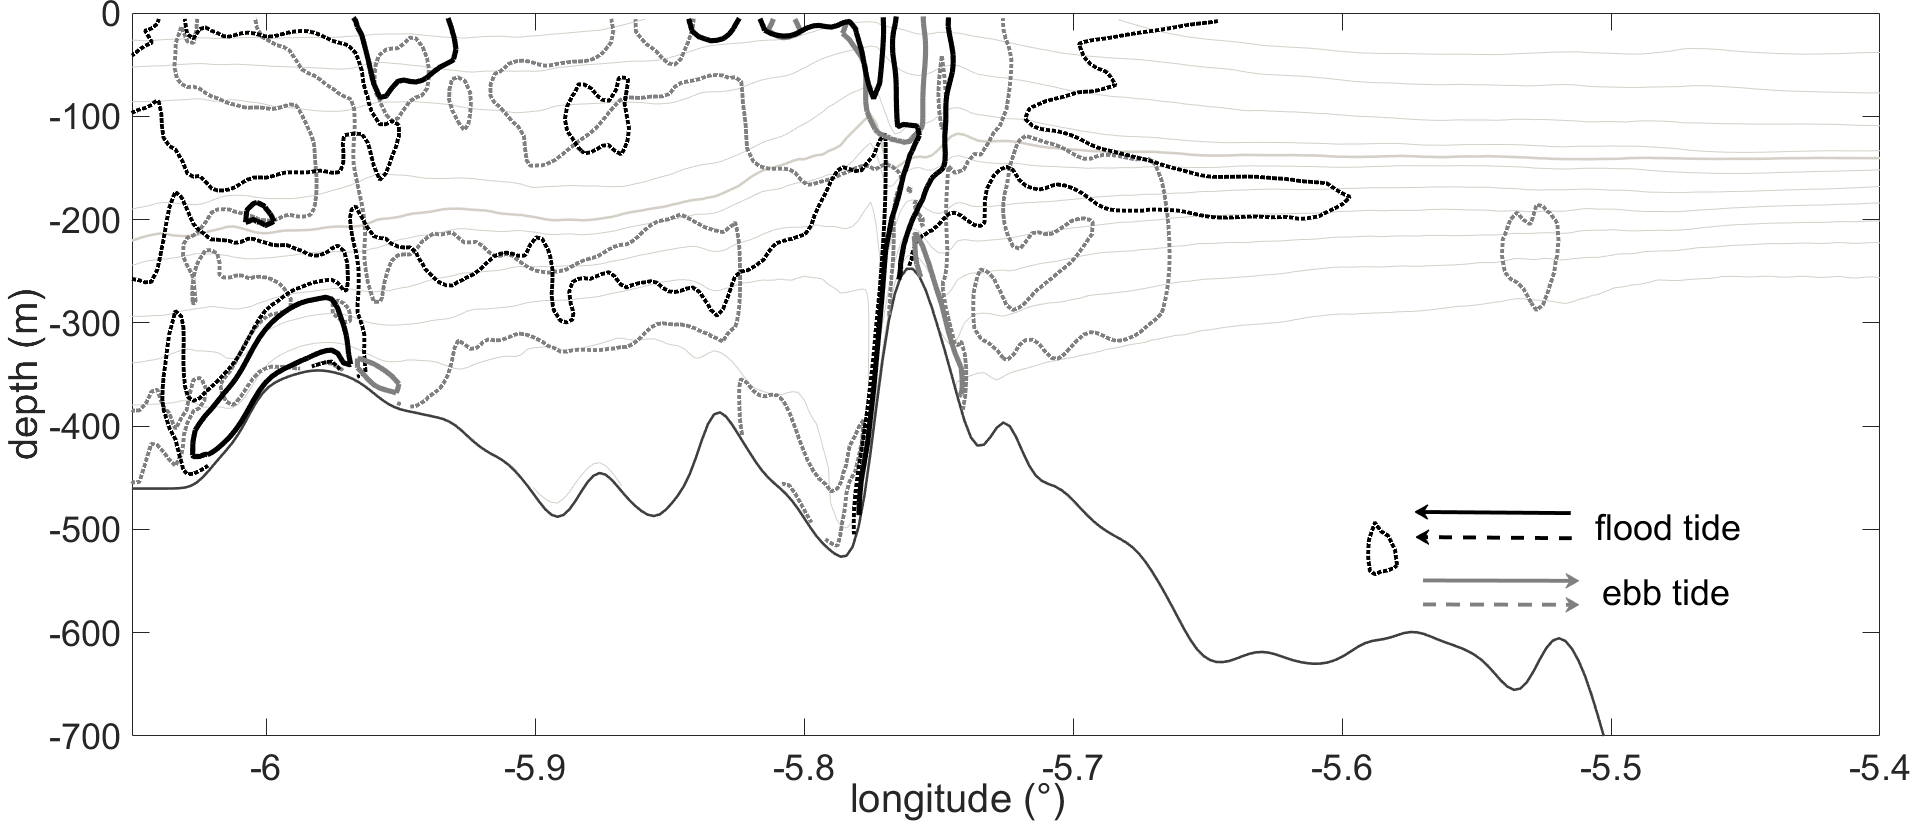
\includegraphics[width=1\textwidth]{./papier2D/Fn_1-2_ref_3T.png}
 \caption{Averaged isopycnal position over 3T (bolded p = -0.7) and region where F > 1 for mode 1 inflow (black) outflow (grey) and for mode 2 inflow (dotted black) outflow (dotted grey) for \textbf{SimRef}. Averages are calculated at maximal inflow and outflow, see figure \ref{hov_ref}.}
 \label{fig_fn_ref}
\end{figure}

A major feature of the dynamics through the Strait of Gibraltar is the so-called "flow criticality" usually characterized with the Froude number ($F$). Several definitions of this non-dimensionnal number can be found in the literature: it can notably be defined for each layer such as in Farmer and Armi (1988) or in Sannino et al (2009). In the present study, the Froude number is simply defined at each grid point as the ratio between the local longitudinal velocity u and the theoretical wave speed $c^*_n$ of the mode-n internal wave, calculated through modal decomposition for each point of the x-axis (see Appendix for details).

Small values of the Froude number ($F < 1$) define a "subcritical" regime, intermediate values ($F \approx 1$) a "critical" regime, and large values ($F>1$) a "supercritical" regime. Hydraulic control appears during the flow transition from subcritical to supercritical and persists when and where large Froude numbers are found. As such, since hydraulic control depends on the current, the existence at a given point of a control can change in time, due in particular to the tidal cycle.

At CS, the tidal current amplitude is of 0.8 m/s. This is sufficient to reverse both the upper-layer mean inflow and lower-layer mean outflow in configurations \textbf{SimAllCor}, \textbf{SimNoCor}, and \textbf{SimRef}. 
%This can be seen in fig.\ \ref{figtransportref} for configuration \textbf{SimRef} where 
The transport (not shown) has a tidal component, with lower (upper) layer transport taking positive (negative) values during flood (ebb) tide. 

In figure %s \ref{fig_fn} and 
 \ref{fig_fn_ref} are plotted the closed contours corresponding to a critical Froude number ($F=1$), inside which the flow is supercritical. The longitudinal velocity fields (u) are taken at maximum outflow (pink and red) at $t = 8.5\ T$ and maximum inflow (cyan and blue) at $t = 9\ T$.
Equivalent maps of supercritical regions can also be plotted for configurations \textbf{SimAllCor} and \textbf{SimNoCor} (not shown).
 The wave speeds are calculated from %the stratification after 70 h for configurations \textbf{SimAllCor} and \textbf{SimNoCor} (figures \ref{fig_fn}.a and b), and from 
 a 3T-time-averaged stratification.% for configuration \textbf{SimRef} (figures \ref{fig_fn_ref}).

First of all, we can see that the supercritical zones for mode 1 are located in the neighborhood of Camarinal and Espartel sills. For all three simulations the control of mode-1 waves occurs on the western slope of CS and ES during the ebb tide. In configuration \textbf{SimNoCor} this extends to the secondary sill of Tanger Bassin. During the ebb tide, the flow is supercritical for mode 1 in both configurations \textbf{SimRef} and \textbf{SimAllCor} on the eastern slope of CS and in \textbf{SimRef} in the neighborhood of ES. Otherwise, the flow is supercritical in the upper layer over CS for all simulations.

Due to the definition of the internal-wave speed (it decreases with mode number n), if supercritical for mode 1, the flow is also supercritical at the same points for mode 2. The regions of supercritical flow for mode 2 can then extend both horizontally and vertically, especially in the pycnocline (see for exemple in figure \ref{fig_fn_ref} during the flood tide).% For example, in configuration \textbf{SimNoCor}, the control spreads on the eastern slope of CS (over bathymetry anomalies).
A supercritical zone for mode 2 can also occur where no mode-1 control is present which is the case in the lower layer at the end of TN during flood tide for the three configurations and during ebb tide for configuration \textbf{SimAllCor}. During the ebb tide this supercriticality of the flow at TN seems to be closely linked to the presence of the mode-1 soliton at the same location. Indeed, the currents induced by mode-1 large amplitude waves can be larger than mode-2 propagation velocities.  

Farmer and Armi (1988) found persistent controls for mode 1 at ES, CS and TN. With their numerical model, Sannino et al. (2009) found only periodical appearances of such controls, except at ES where it is persistent. The discrepancy is probably for a large part due to the method and data used to calculate the composite Froude number. Here, our results indicate a tidal periodicity of mode 1 at both CS and ES but never in TN. The latter is logical since our model does not integrate the convergence of the Strait's lateral boundaries. The lack of perpetual control at ES (which, in the literature, extends to the supercriticality of the Mediterranean outflow away from the strait) may come from the crudely imposed stratification. 
%Mode-2 supercritical regions is more present in the pycnocline (or interface layer). It can also occur at positions where a mode 1 is present in the along-strait (u) velocity field, as is the case at TN (\color{blue} what did you mean by ``structure of the supercritical regions''? I shortened the sentence make sure you agree with the result.\color{black}). 
Comparisons are difficult as Froude number and hydraulic control can be defined in various ways. Furthermore, the "maximal exchange" solution is not clearly defined for models with more than two layers in the Strait. One way to localize these controls could be to follow the motion of the isopycnals.

In figure \ref{CV_ressaut}.a the density field for configuration \textbf{SimRef} is plotted at CS during maximum outflow at t = 8.5 T and through the transition to ebb tide in figures \ref{CV_ressaut}.b to \ref{CV_ressaut}.d.

In figures \ref{CV_ressaut}.a to \ref{CV_ressaut}.c, a depression of the isopycnals can be observed immediatly downstream of CS. This hydraulic jump corresponds to the flow transition from supercritical to subcritical in figure \ref{fig_fn_ref}. In figure \ref{CV_ressaut}.a on the other side of CS the isopycnals are spread in the water column over the secondary crest of CS, looking like a trapped mode-2, but it has disappeared in figure \ref{CV_ressaut}.b.

In figure \ref{CV_ressaut}.c and \ref{CV_ressaut}.d, the tidal current slackens and then its orientation changes. In figure \ref{CV_ressaut}.c a bore crosses the crest of CS and it has then steepened in figure \ref{CV_ressaut}.d when a mode-2 disturbance is crossing CS.% This latter passage is featured in the instantaneous transport of fig.\ \ref{figtransportref}. Indeed, during the very first hours of the flood tide, the upper layer transport has a sudden minimum corresponding to a maximum of the upper layer transport \color{blue} (reformule...) \color{black}: this could correspond to the signature of the mixed waters in mode 2. This may appear more clearly if the transport of the interfacial layer was separated from the transports of the upper and lower layers.\\

Overall, the hydraulic jump that apparently develops west of CS during the flood tide remains during four hours in configuration \textbf{SimRef}. It appears not long after low water. Between figures \ref{CV_ressaut}.a and b the amplitude of the hydraulic jump (displacement of isopycnal $-0.5\ kg.m^{-3}$) increases for example from 100 m to 150 m. It decreases afterwards as a mode-1 wave and then a mode-2 wave are generated and propagate eastward. Smaller jumps occur during flood tide on the estearn side of CS, as well as over ES. \\


\begin{figure}[!h]
\begin{subfigure}{0.5\linewidth}
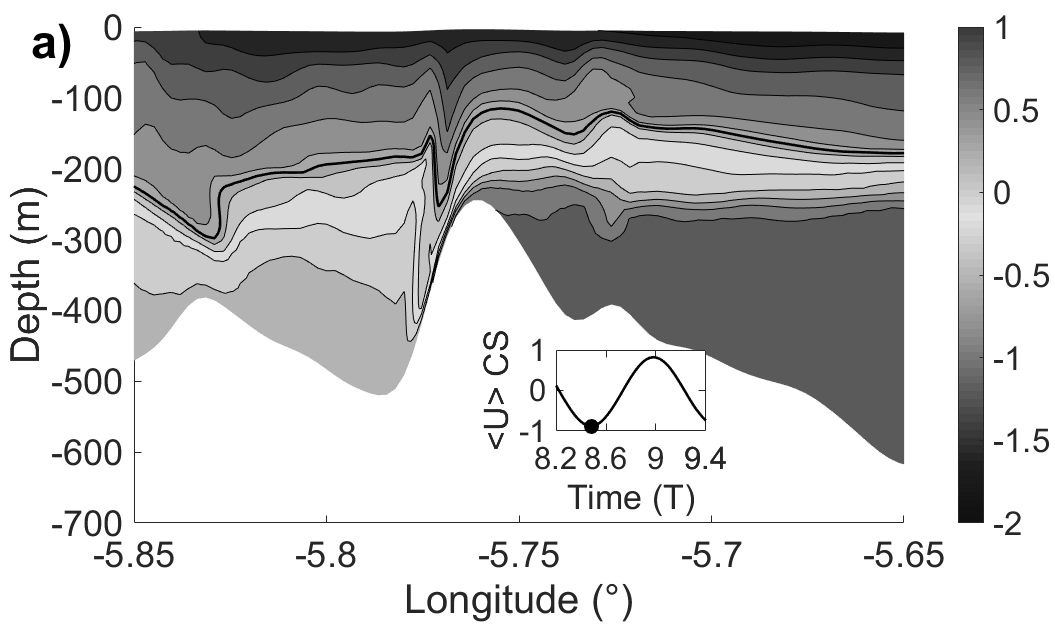
\includegraphics[width=\textwidth]{./papier2D/RW_J4_9h12_ref.png}
\end{subfigure}
 ~
\begin{subfigure}{0.5\linewidth}
  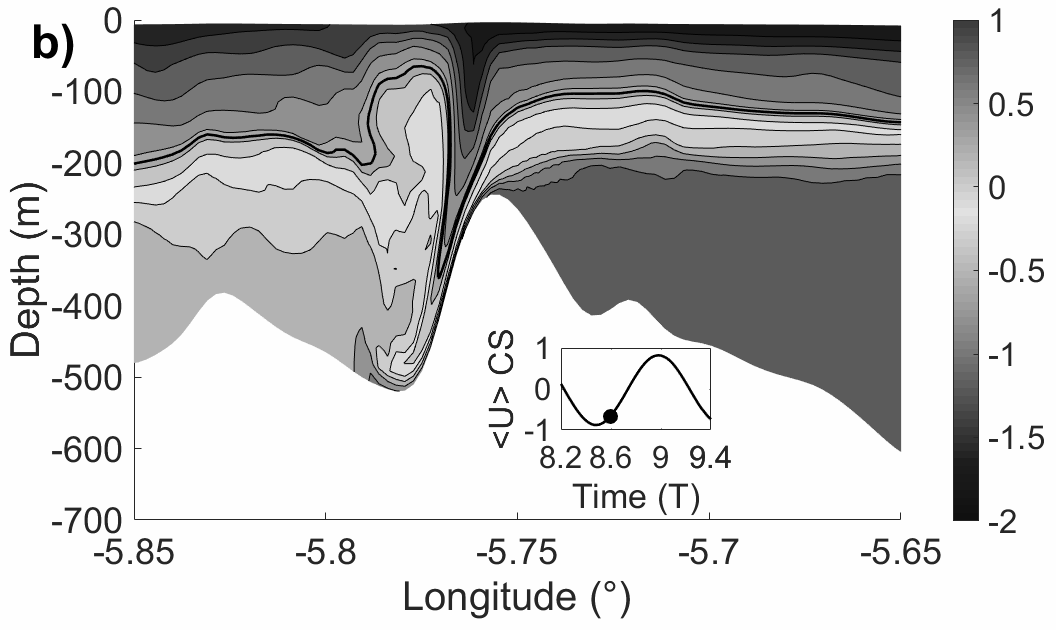
\includegraphics[width=\textwidth]{./papier2D/RW_J4_10h36_ressautebb.png}

\end{subfigure}
 
\begin{subfigure}{0.5\linewidth}
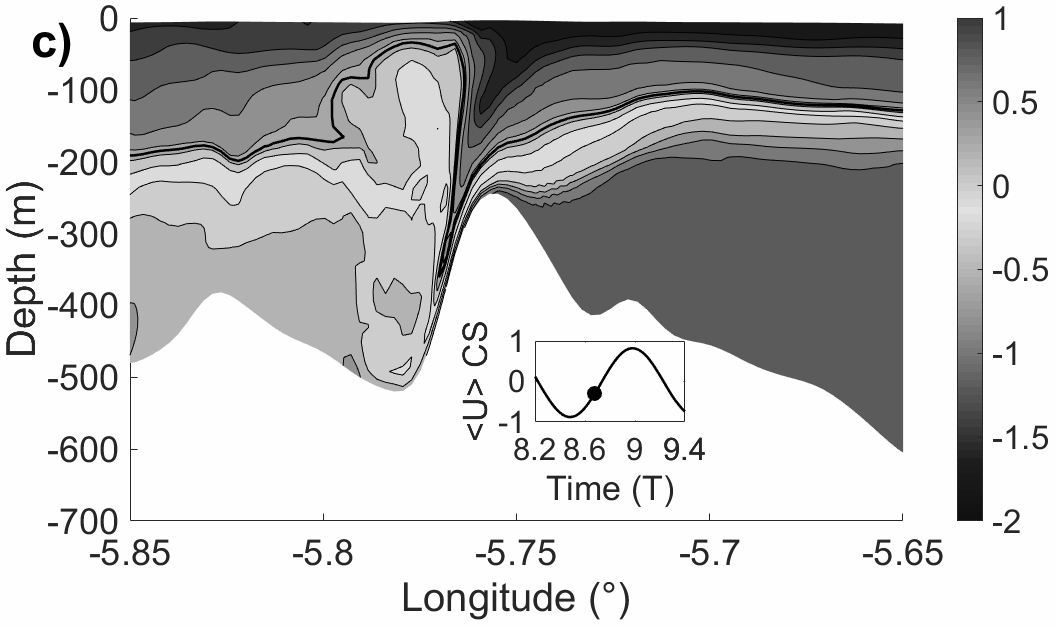
\includegraphics[width=\textwidth]{./papier2D/RW_J4_11h36_deferl.png}

\end{subfigure}
 ~
\begin{subfigure}{0.5\linewidth}
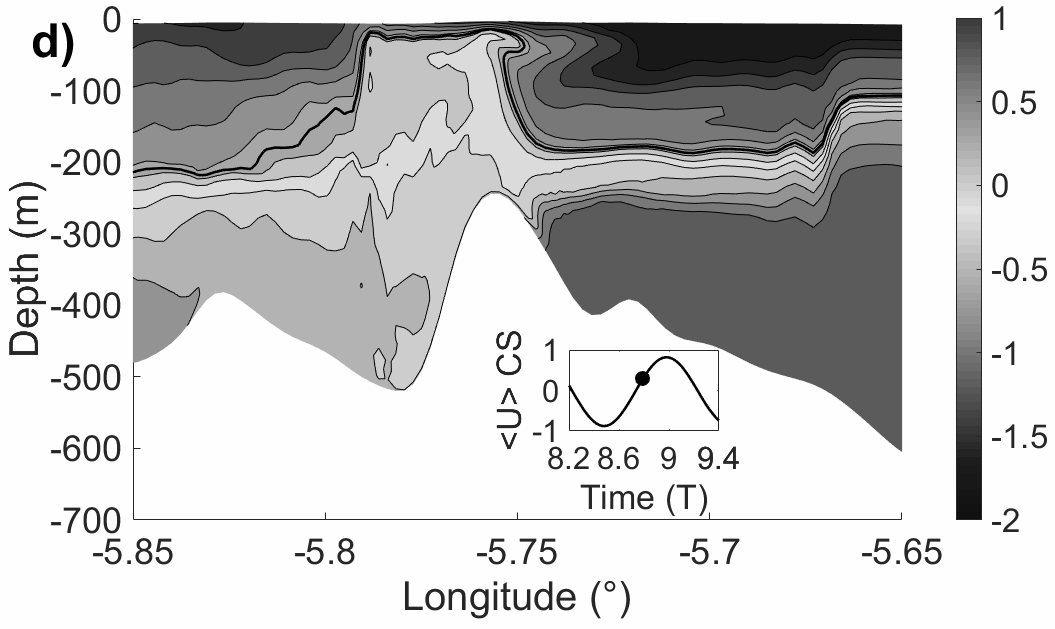
\includegraphics[width=\textwidth]{./papier2D/RW_J4_13h_gen_mod1.png}

\end{subfigure}
 \caption{Density fields of \textbf{SimRef} zoomed over CS, bolded isopycnal: $\rho'\ =-0.5\ kg/m^3$ at t=8.5 T (a), t=8.6 T (b), t=8.7 T (c) and t=8.8 T (d)}
 \label{CV_ressaut}
\end{figure}
 

\paragraph{Internal tide dynamics}
%%%%%%%%%%%%%%
% Figure 5
%%%%%%%%%%%%%%
\begin{figure}[!t]
\centering
\begin{subfigure}{1\linewidth}
\centering
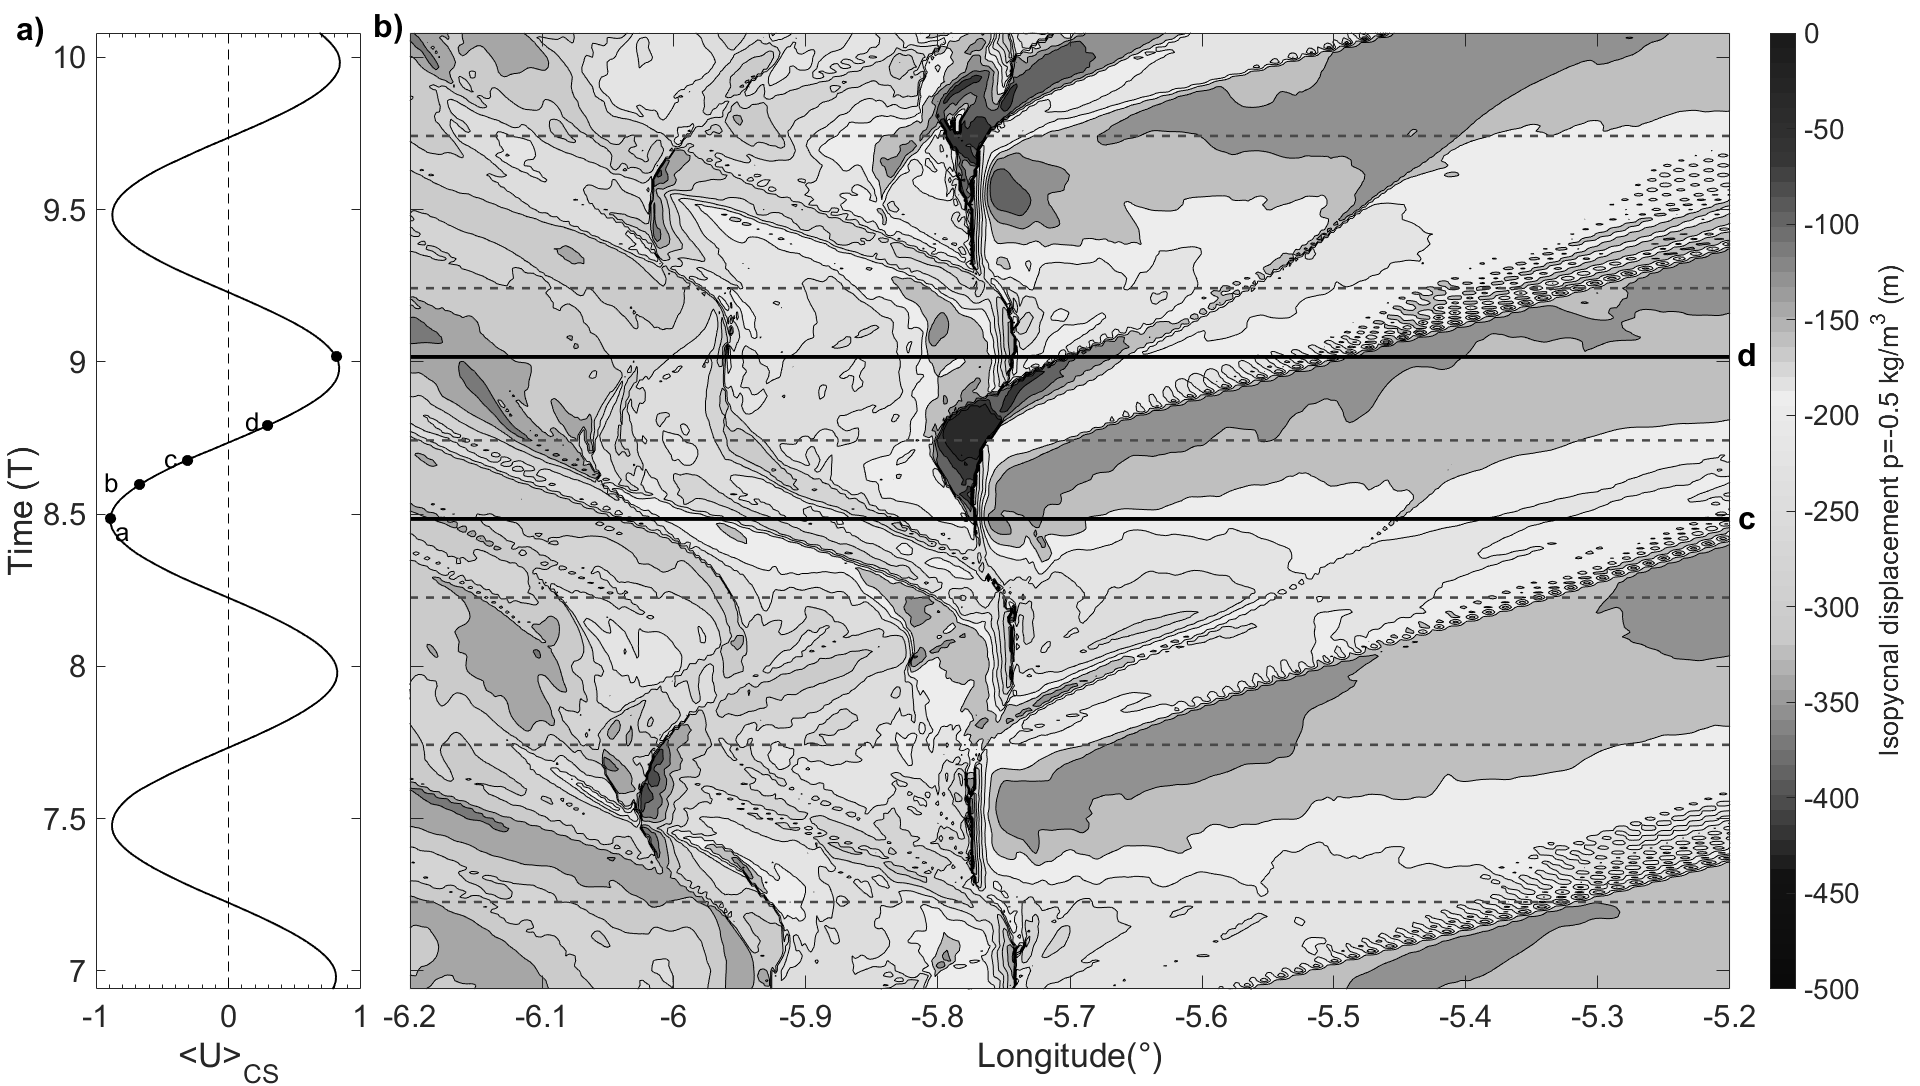
\includegraphics[width=1\linewidth]{./papier2D/hov_ref_-05.png}
\end{subfigure}

\begin{subfigure}{1\linewidth}
   \centering
  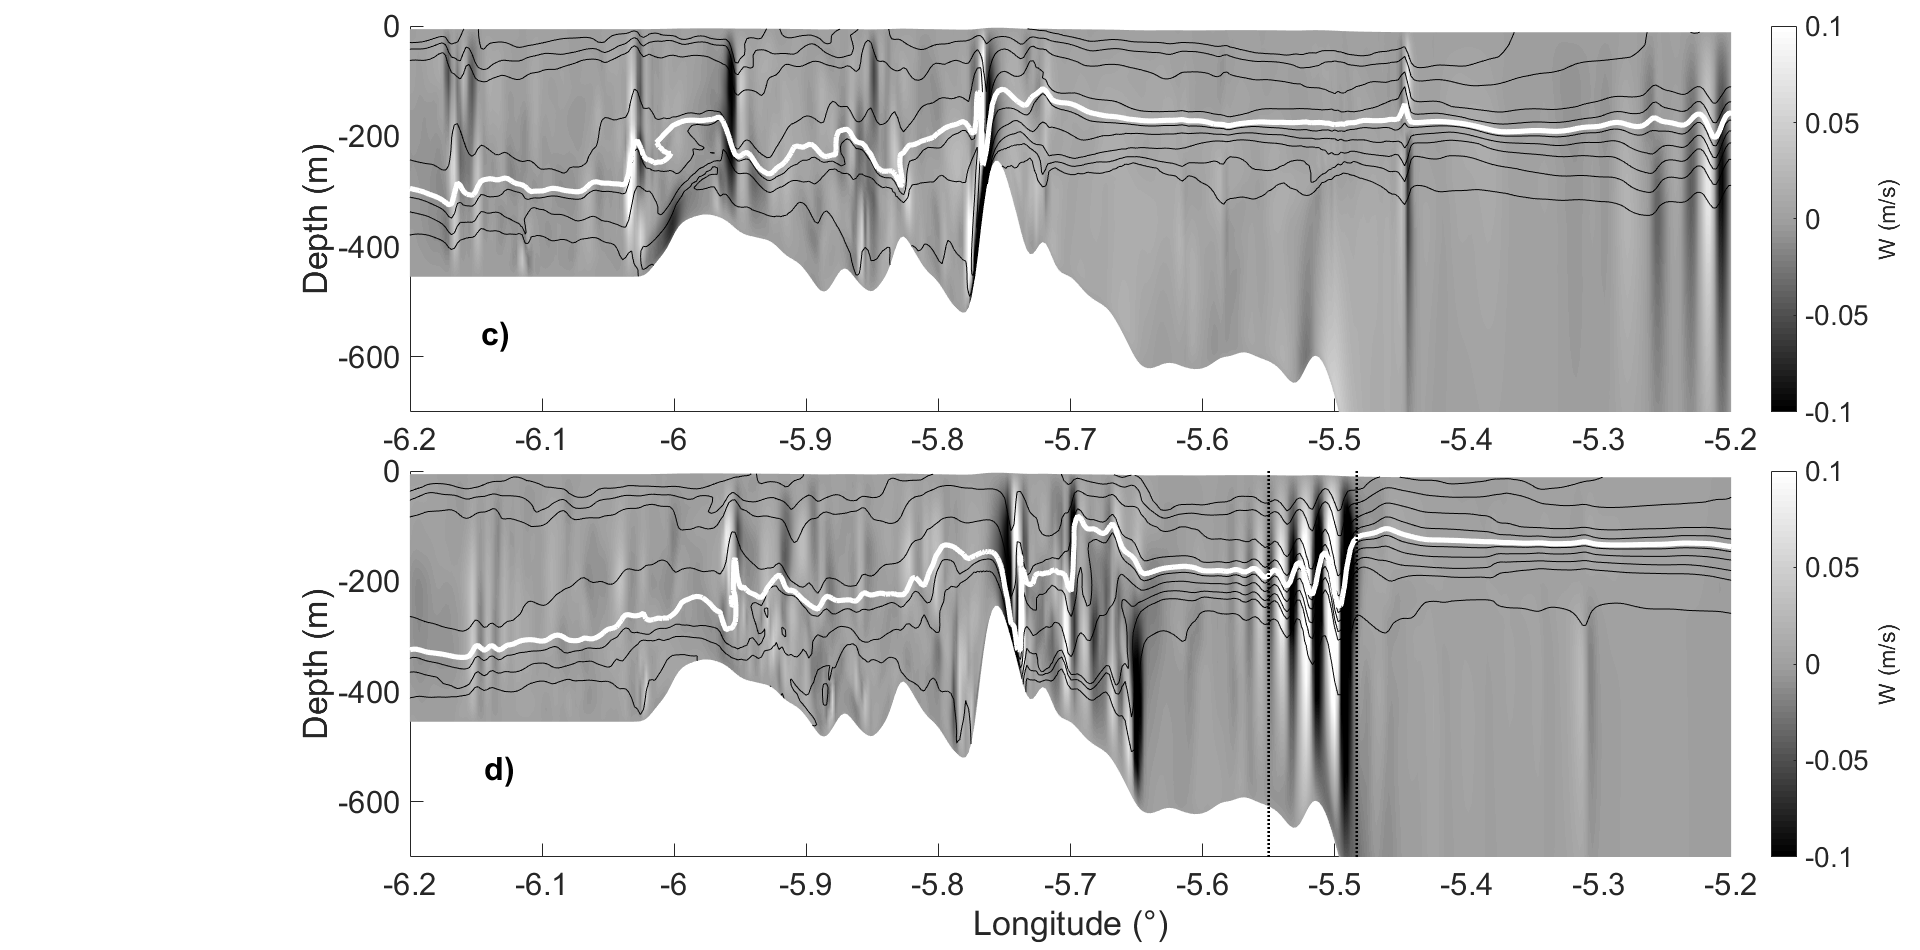
\includegraphics[width=\textwidth]{./papier2D/RW_J4_9h12-15h48.png}
\end{subfigure}
 \caption {(a) vertically averaged current over CS (dots indicate times of plots in figure \ref{CV_ressaut}). (b) Space-time diagram of the vertical displacement of isopycnal $=-0.5 \ kg/m^3$ of \textbf{SimRef}. The dashed lines indicate transition between ebb tide and flood tide, the black lines indicate the times of the two bottom panels. (c) and (d) vertical velocity field and isopycnals at the times indicated in panel (b). In white is the isopycnal $\rho'\ =\ -0.5 \ kg/m^3 $.}
 \label{hov_ref}
\end{figure}

\indent Figure\ \ref{hov_ref}.b is a space-time diagram of the vertical displacement of the isopycnal surface $-0.5\  kg/m^3$ in \textbf{SimRef}. Regions of sharp density gradients can be identified periodically in the region of CS near -5.76°. They correspond to the generation of hydraulic jumps. The propagation of mode-1 and mode-2 large amplitude internal waves can be then followed by the tilt of the isocontours. In this diagram, the slopes correspond to the wave's propagation speed. There are differences from one tidal cycle to the other since, with the mixing, the isopycnal surface gets higher in the pycnocline. In the following, we focus on the tidal cycle t= 8.5 T - 9.5 T (third cycle after the end of the spin-up phase), the corresponding tidal-averaged shear and stratification conditions are shown in figure \ref{fig_current} and figure \ref{fig_fn_ref}.

East of CS a mode-1 wave is generated two hours after the maximum outflow, first as a bore over CS with an amplitude of 100 m and a speed of about 1.3 m/s (as can be seen in figure \ref{CV_ressaut}.d). It continues propagating east in TN as a train of 2 to 3 solitary waves, the first of which has an amplitude of 110 m and a speed of 1.6 m/s. The amplitude of the train of solitons momentarily increases and exceeds 150 m as it propagates over the slope at -5.5° in TN (still with inflowing tidal current).

This ISW train is followed by a mode-2 bore which is generated during the release of the hydraulic jump at high water tide. It goes through CS at a speed of 0.6 m/s and then 0.8 m/s in the shallowest part of TN as a new hydraulic jump remains on the east slope of CS (figure \ref{hov_ref}.d). Its amplitude is then of 100 m. 

With the transition to flood tide, the eastward propagating mode 1 continues its way over the deepest part of the domain. There, the train keeps on being dispersed: when the mode-1 ISWs leave the domain, 7 solitons can be found in the train. The mode-2 bore amplitude decreases and is slowed down by tidal advection: this is for instance the case for a mode-2 bore released during the previous tidal cycle and whose induced velocity signature is still recognizable in the eastern, deepest part of the domain (figure \ref{hov_ref}.c and d).

The signatures of other large amplitude internal waves are visible in the domain west of CS. The western most is a mode-1 wave with an amplitude smaller than the eastward propagating one. It was generated one tidal cycle before by the hydraulic jump in the same way as the train appearing east of Camarinal sill in figure \ref{hov_ref}.

%Figure \ref{figRWna} presents the vertical velocity field and the isopycnals at the same time as figure \ref{hov_ref}.d, but for the configurations \textbf{SimAllCor} and \textbf{SimNoCor}.  
The same figures as in figure \ref{hov_ref} for configurations \textbf{SimNoCor} and \textbf{SimAllCor} can be plotted to follow the forecasted wave dynamics (not shown). In term of speed of the mode-1 wave propagating east of CS, configurations \textbf{SimRef} and \textbf{SimNoCor} are very similar. However, in \textbf{SimNoCor} the amplitude of both mode 1 and mode 2 are smaller and the train of solitons develops only after the wave has descended the slope in eastern TN.

In configuration \textbf{SimAllCor} the speed of the mode 1 wave is of 1 m/s, less than in the other two configurations. The amplitude of the first mode-1 wave is greater and can exceed 200 m. Dispersive effects generate waves to the train in the eastern, deeper part of TN when the wave propagates in the stratified surface layer away from the surface front of Atlantic water.

% \color{red} On peut enlever figure \ref{figRWna}. \color{blue} idem... Je suis d'accord, il faut faire des choix!\color{black}
% %%%%% Figure
% \begin{figure}[!t]
% \centering
% \includegraphics[width=1\linewidth]{comp_15h48_allcor_nocor.png}
% \caption{Field of vertical velocity and isopycnals (white isopycnal $\rho'$=-0.5) in configurations \textbf{SimAllCor} (a) and \textbf{SimNoCor} (b) at the same time as fig.\ref{hov_ref}.d}
% \label{figRWna}
% \end{figure}

In figure \ref{hov_ref}.d %and on both panels of figure \ref{figRWna}
, vertical lines in TN are plotted. They refer to measurments in Farmer and Armi (1988): the lines indicate indeed the position of the two baroclinic modes for each tidal cycle. The right (left) vertical line corresponds to mode 1 (mode 2) three and a half hours after high water, in agreement with the simulations.

In configuration \textbf{SimRef} the distance between the two modes is twice as large (figure \ref{hov_ref}). Mode 1 is well positioned but mode 2 is just entering TN. The same distance between mode 1 and mode 2 can be observed in configuration \textbf{SimNoCor}, whereas the distance between the two modes is closer to observations in configuration \textbf{SimAllCor} though the waves arrive at this positions with a delay. The mode 1 is better positioned in \textbf{SimRef} and \textbf{SimNoCor}.

Based on this measures of wave arrival at various stations, Farmer and Armi (1988) estimated the propagation speed of both mode-1 and mode-2 waves at about 1 to 2.5 m/s for mode 1 and 1 to 1.5 m/s for mode 2. The wave train they observed contained two to three large amplitude waves, the first one having an amplitude of 100 m. 

Other measures in S\'anchez Garrido et al. (2008) estimated a mean propagation speed for the mode-1 waves in TN between 1.2 m/s and 2 m/s with an important diurnal variation.

The mode-1 waves in both the configurations \textbf{SimRef} and \textbf{SimNoCor} have a propagation speed in this range whereas the ones in configuration \textbf{SimAllCor} are too slow and their amplitude is too large.


%%%%%%%%%%%
%\paragraph{Compared dispersion and dissipation with Korteweg-de Vries (KdV) dynamics and satellite images}

%We basically discuss here the contain of Lucie's NumLab to which we can add a comparison with a sequence of Sat images...
%(
\paragraph{Comparison with Korteweg-de Vries (KdV) dynamics}
%)

\begin{figure}[!h]
\centering
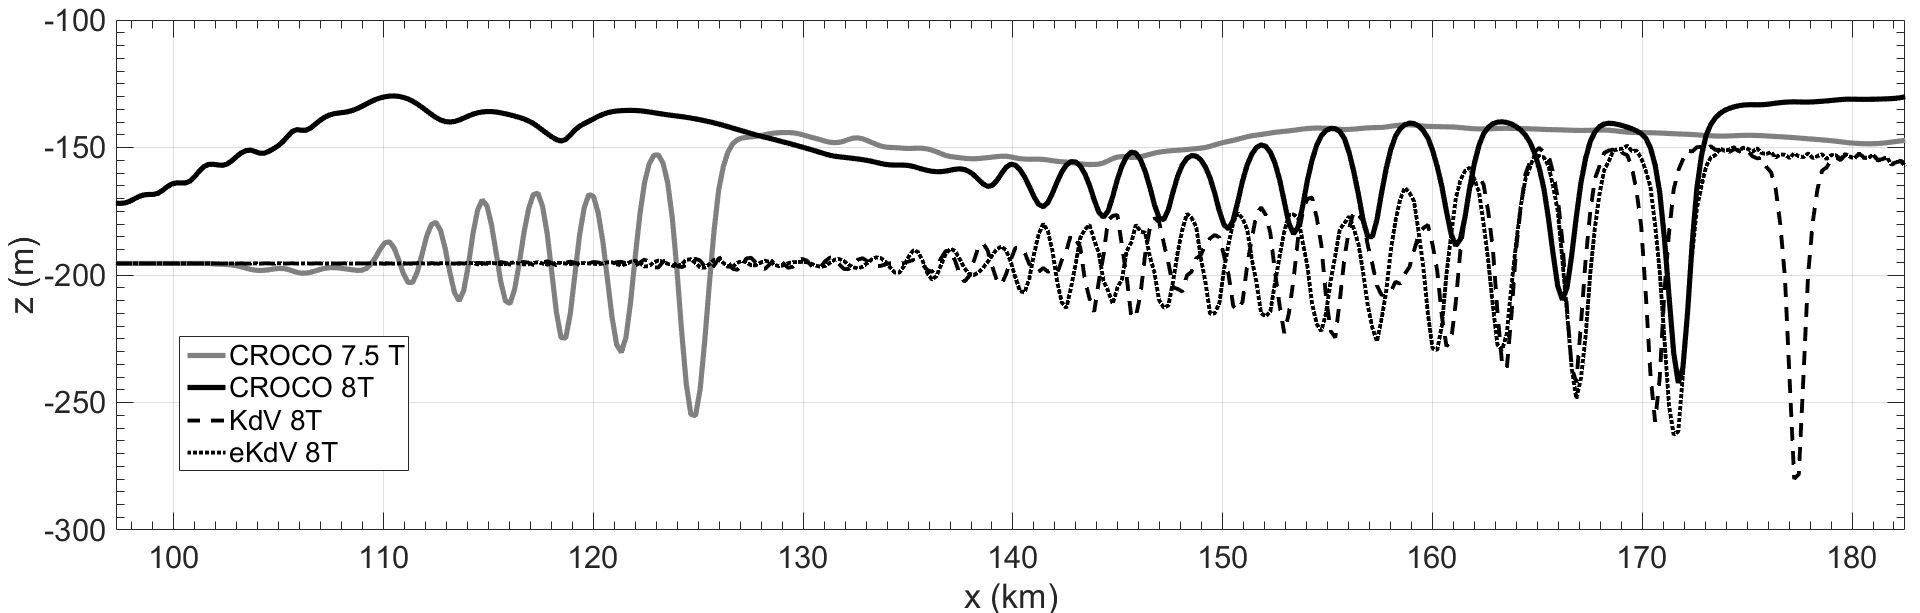
\includegraphics[width=1\linewidth]{./papier2D/exp_kdv_75-8T.png}
\caption{Isopycnal $\rho$'=-0.5 kg/m$^3$ simulated by CROCO-NBQ at t=7.5 T (grey) and t=8 T (black). Evolution of the interface as simulated by KdV (dashed) and eKdV (dotted).}
\label{fig_kdv}
\end{figure}

In previous subsections large amplitude waves propagating over large distance have been compared to available observations. Following many authors (S\'anchez-Garrido et al., 2008, Vlasenko et al., 2009, Sannino et al., 2009b) some of these waves were termed ``ISWs'' for Internal Solitary Waves. We shall now verify if these waves correspond to solutions of the Korteweg-de Vries equation recalled bellow. For these solutions, non-hydrostatic dispersion balances non-linearity. Non-linearity steepens the edge of the wave, whereas non-hydrostatic dispersion is associated to a transfer of energy from large to  small scales, resulting in relatively stable entity called ``solitary'' waves. 

The Korteweg-de Vries (KdV) equation describes the evolution of an infinitely thin interface in a two-layer system with constant bottom topography:
\begin{equation}
\frac{\partial \zeta}{\partial t} 
+c^* \frac{\partial \zeta}{\partial x}
\underbrace{+ \frac{3}{2} \frac{h_1-h_2}{h_1h_2} c^* \zeta \frac{\partial \zeta}{\partial x} }_{A}
\underbrace{+ \frac{1}{6} h_1h_2c^* \frac{\partial ^3 \zeta}{\partial x^3} }_{B}
\underbrace{ - \frac{3}{8}\zeta^2c^*\frac{h_1^2+6h_1h_2+h_2^2}{8(h_1h_2)^2} }_{C}
=0
\label{eq_kdv}
\end{equation}
where $c^*$ is the linear wave speed of small-amplitude internal waves: $c^*=\sqrt{g' h}\ = \ R*f$ and $\zeta$ is the vertical displacement of the interface. $g'$ and $h$ where previously defined in subsection 3.1.

The first two terms on the left hand side of (\ref{eq_kdv}) correspond to a classical propagation equation of a small-amplitude, linear, interfacial wave propagating in the x-direction at a velocity $c^*$. The third term on the left hand side, (A) in (\ref{eq_kdv}), is a first-order approximation (in term of amplitude) of the non-linear advection. The following term (B) is a dispersive term.

The fifth term (C) is a higher-order non-linear term associated to a second order development of advection. This complete equation (\ref{eq_kdv}) will be referred as the "extended KdV (eKdV)", whereas without term (C) it will be simply referred as KdV (Dossmann et al. 2012). 

The large amplitude waves simulated in the previous subsection are now compared to the solutions of the (e)KdV equation to make sure they are ISW. To this aim, we run a new simulation, called \textbf{SimRef+}, with the characteristics given in table \ref{tabsimref} except that (i) the eastern boundary is further east (845 horizontal points, $\rho_0\ =\ 1033.9 \ kg/m^3$) and (ii) the tidal forcing is stopped after only 7.25 periods. The first eastward-propagating train of mode 1 waves generated by the tide at CS in CROCO-NBQ is compared with the propagation given by numerically integrating the (e)KdV equation (\ref{eq_kdv}).

The vertical displacement of isopycnal $\rho'\ =\ -0.5\ kg/m^3$ is extracted at $t_0\ =\ 7.5\ T$ when the mode-1 ISW train is propagating over a region of constant depth H = 890 m west of TN and is represented in figure \ref{fig_kdv}. At that time, the distance between the first and second wave is of 3.3 km, the first wave of the train has an amplitude of 104 m and the train has 6 waves. This isopycnal is chosen as the initial state for the (e)KdV framework. The mode 1 linear propagation speed is computed from this initial state: $c^*\ =\ 1.53\ m/s$.

Figure \ref{fig_kdv} compares the depth of interface obtained at $t\ =\ t_0\ +\ 0.5\ T$ with the KdV and eKdV equations with the position of the $-0.5\ kg/m^3$ isopycnal surface in \textbf{SimRef+}. For the CROCO-NBQ simulation, the distance between the first two waves of the train is 5.5 km with an amplitude of 104 m for the first trough. The train is made of ten waves. It is followed by a disturbance caused by a smaller amplitude internal wave that was generated during the inflow.

In figure \ref{fig_kdv}, the second-order advection term in eKdV adds dissipation. This term slows down the wave and reduces its amplitude. As a result, the speed of the first wave and its amplitude are coherent with the ones simulated in CROCO-NBQ. The distance with the second wave of the train is also closer to CROCO-NBQ in eKdV (4.6 km) than in KdV (6.9 km). In both KdV and eKdV, the train has more waves than simulated by CROCO-NBQ.

The shape and evolution of the large amplitude waves appearing in \textbf{SimRef+} are consequently close to the one predicted by the (e)KdV equation (\ref{eq_kdv}) confirming that (i) this large amplitude wave propagate as ISW and (ii) CROCO-NBQ provided an accurate simulation of ISW in realistic conditions. Both the NH-kernel (for NH dispersion) and the advection schemes (for non-linearity) of the code are concerned.\\


%----------------------------------------------
\paragraph{Comparison with Satellite images}
%\begin{wrapfigure}[16]{r}{0.5\textwidth}
\begin{figure}[!h]
 \centering
 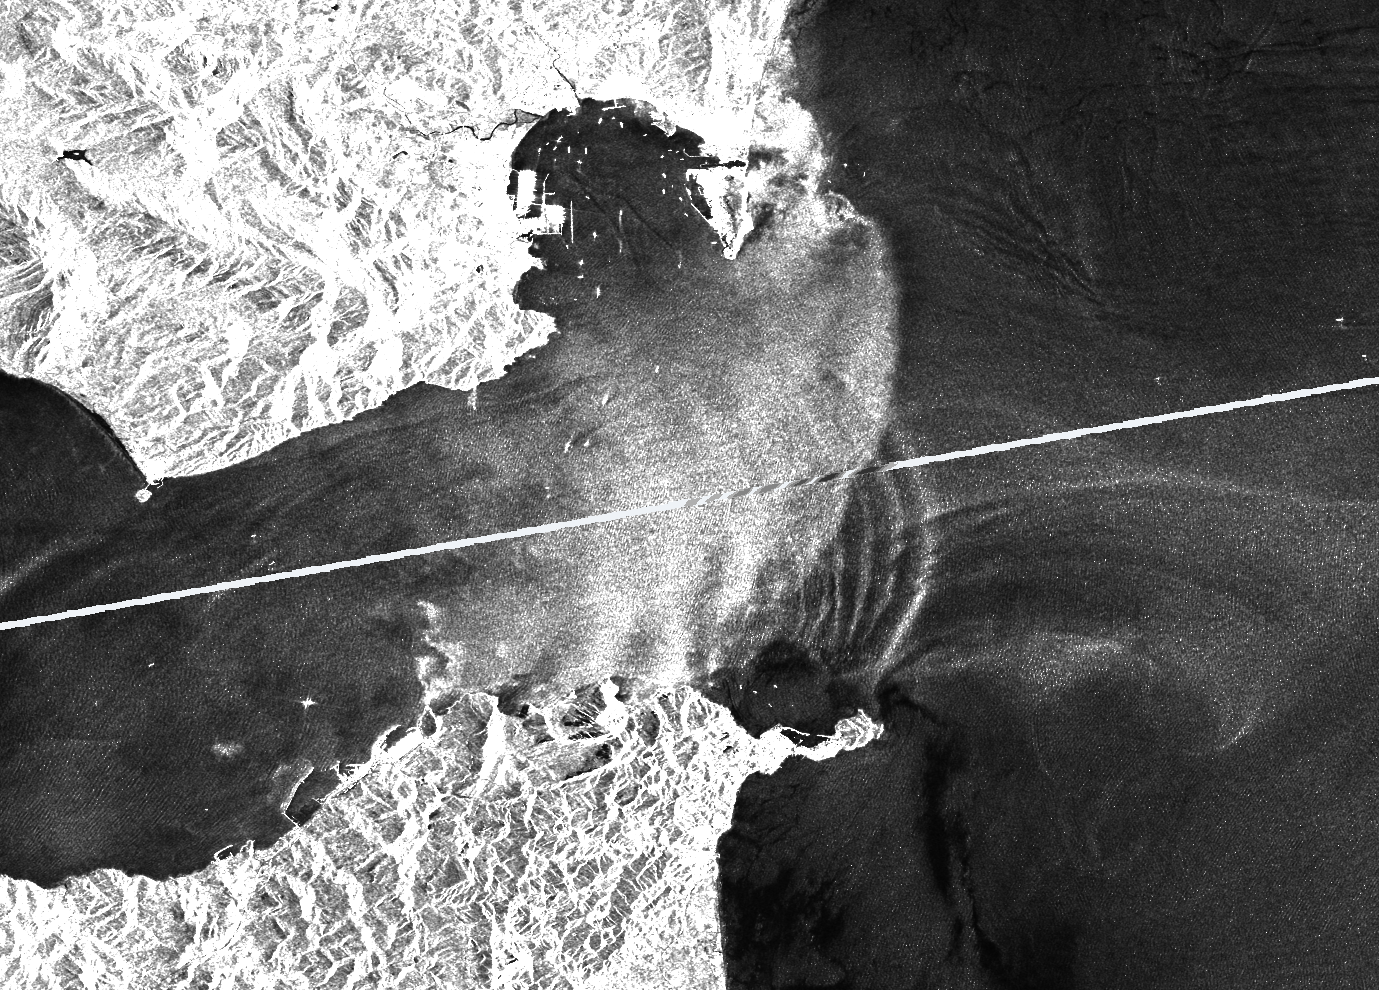
\includegraphics[width=0.45\textwidth]{./papier2D/sat_2dref_20042016_zoom.png}
 \caption{SAR image of Sentinel 1 the 20/04/2016 at 6h27 UTC and absolute value of the slope of $\eta$ in \textbf{SimRef} (in red the slope is non-zero). }
 \label{sat2d}
\end{figure}
%\end{wrapfigure}

Yet another comparison of the ISW propagation can be made with SAR\footnote{SAR: Synthetic Aperture Radar} satellite data (Alpers, 1985). Figure \ref{sat2d} presents an image of the recently launched, high-resolution, Sfentinel 1 SAR that shows a train of mode-1 ISW leaving the strait at a time corresponding to low-water. The absolute value of the gradient of the free-surface elevation ($\vert \partial \eta / \partial x \vert$) is superposed at $t = 7.25\ T$ in simulation \textbf{SimRef}. The wavelength of the first wave in the simulation can for instance be deduced by measuring the distance between the first and third black patch on the transect in figure \ref{sat2d}.\color{black}

In the satellite data, a distance of 1.5 km is measured between the first two waves, of which we can count 6 in total. By comparison, there are also 6 waves in the simulation, but they have a longer wavelength with a distance of 2.6 km between the first two.

The discrepancy in position can be explained by the tidal amplitude which is smaller in the simulation. As a consequence, the solitary waves propagated more slowly (Farmer and Armi, 1988). However, the larger wavelength means that the 2D configuration is too dispersive, maybe in part because there are 3D effects (such as possible interactions with the strait boundaries) which reduce the dispersion and are not taken into account.\\


%%%%%%%%%%%%%%%%%%%%%%%%%%%%%%%%%%%%%%%%%%%%%%%%%%%%%%%%%%%%%%%%%%%%%%%%%%%%%
\subsection{Sensitivity to physical factors}
The so-called \textit{Reference configuration} proposed in the previous subsection is based on several physical and numerical choices as well. We now investigate the impact on the strait's small-scale dynamics of both physical (topography and amplitude of the tides) and numerical (spatial resolution and hydrostatic approximation, next section) parameters. 

%\paragraph{Physical factors}

%%%%%%%%%%%%%%%%%%%%%%%%%%%%%%%%%%%%%%%%%%%%%%%%%%%%%%%%%%%%%%%%%%%%%%%%%%%%%

%----------------------------------------------------------------------------
\paragraph{Topography}
%----------------------------------------------------------------------------
\label{TestPhy}

\begin{figure}[!t]
\centering
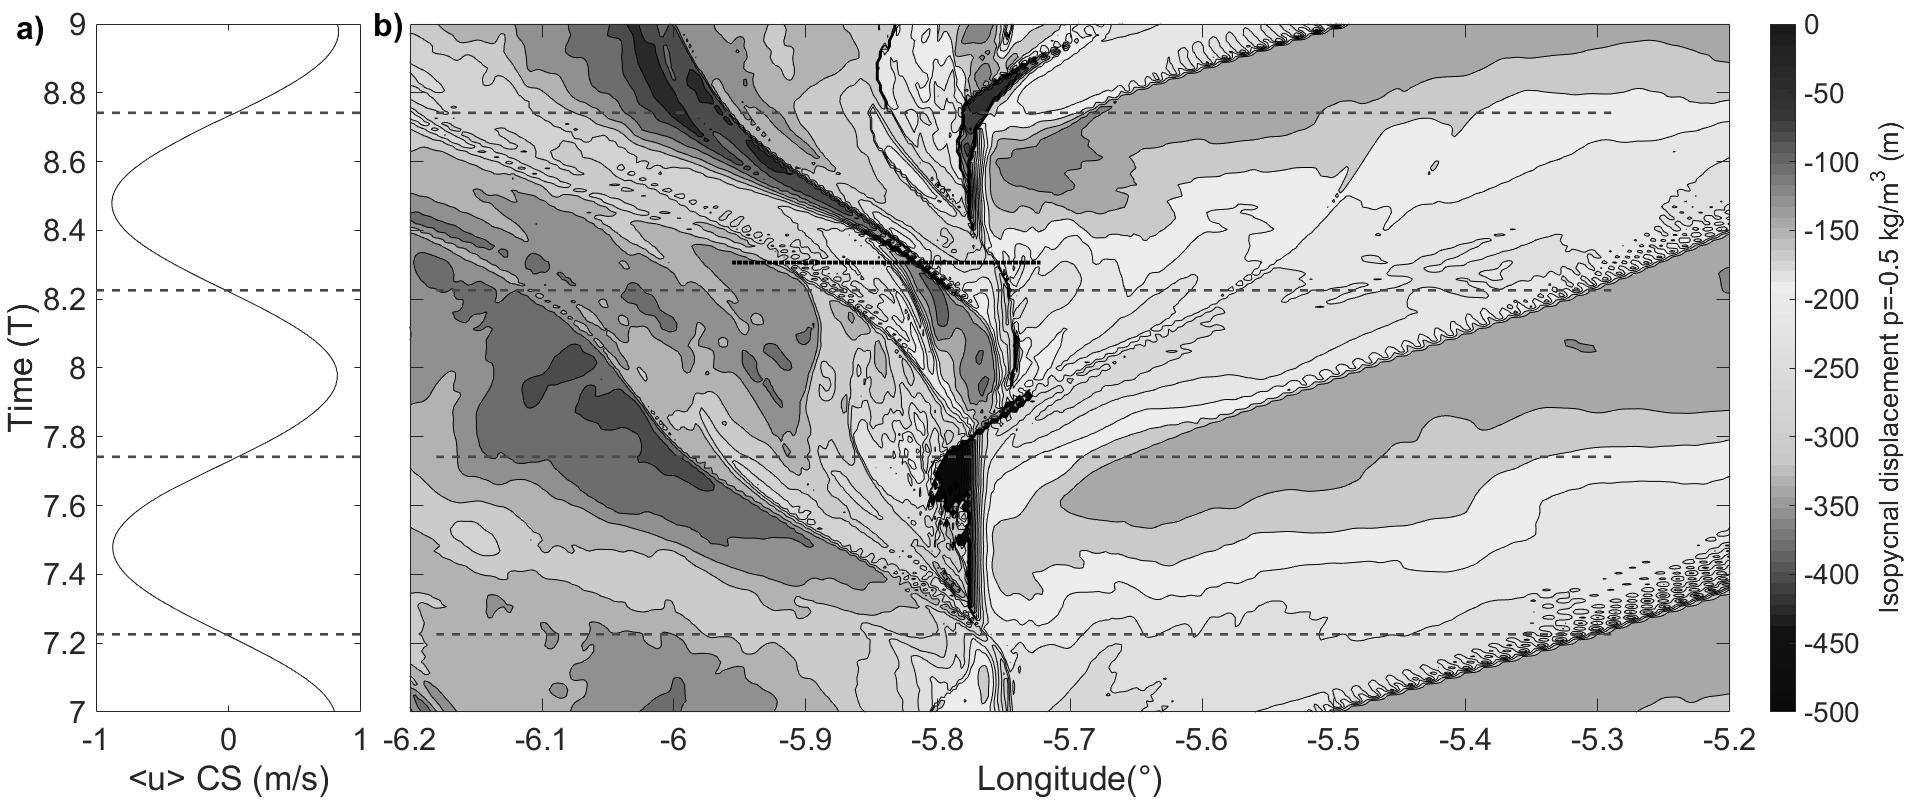
\includegraphics[width=1\linewidth]{./papier2D/hov_p-05_CS.png}
\caption{Same as fig \ref{hov_ref}.a and b for \textbf{SimA}.}
\label{hov_CS}
\end{figure}
\begin{figure}[!h]
\centering
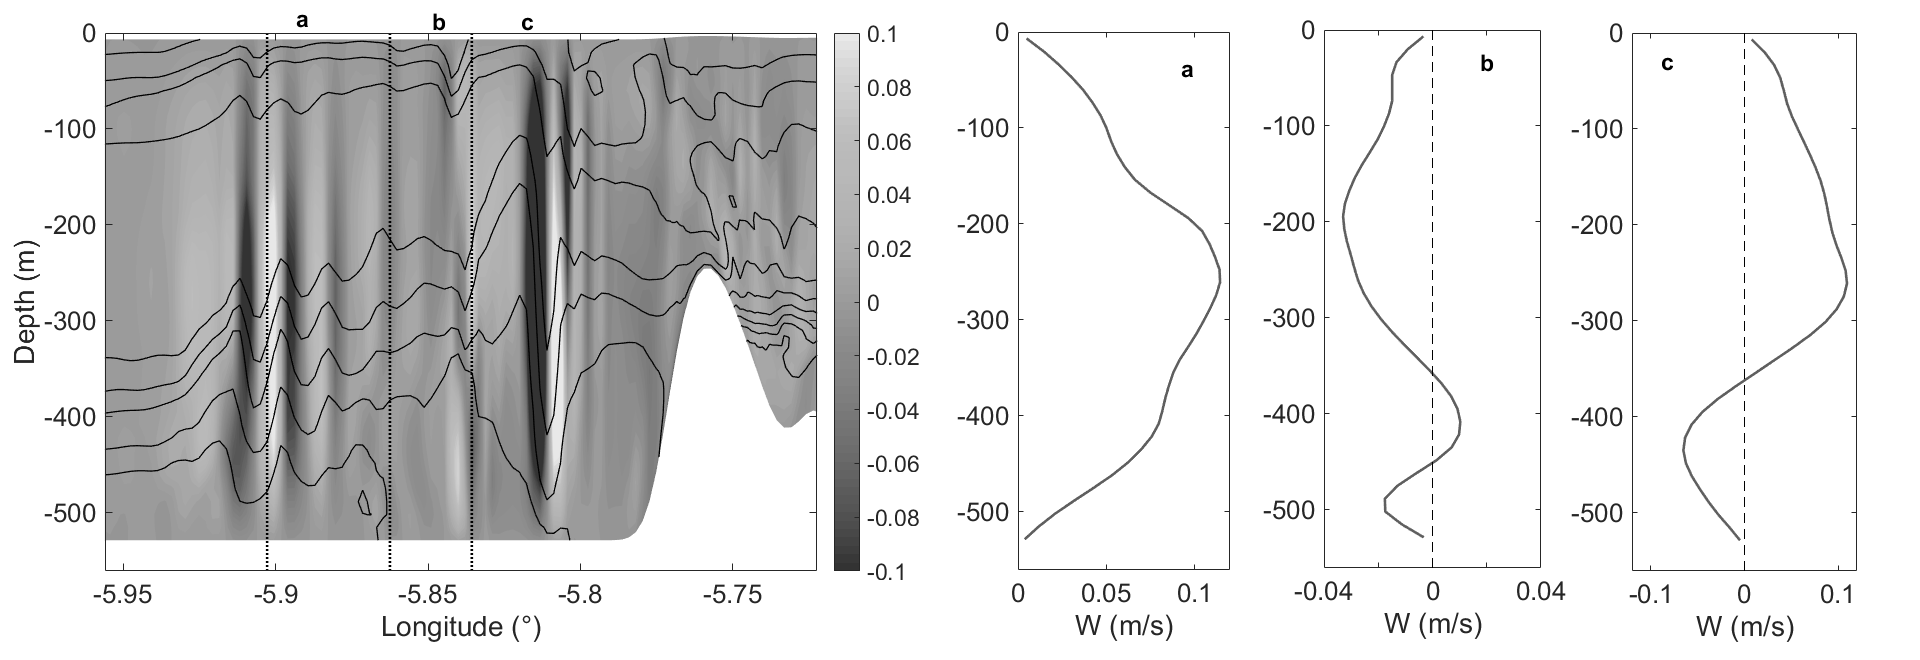
\includegraphics[width=1\linewidth]{./papier2D/w_it515_modes_CS.png}
\caption{Left : field of vertical velocity  and isopycnal contours in \textbf{SimA}. Right: profiles of vertical celerity in the water column.}
\label{figCS_2}
\end{figure}

A first sensitivity simulation, \textbf{SimA}, is run with the same characteristics as the Reference configuration (\textbf{SimRef}, table \ref{tabsimref}), except that all topographic features apart from the bathymetry of CS are smoothed over. East (west) of CS, the resulting depth is constant and is equal to -620 m (-530 m). The reference density is $\rho_0\ =\ 1033.5\ kg/m^3$. The objective is to isolate the effect of CS, especially on the western side of the domain.

Figure \ref{hov_CS} presents the space-time evolution of the vertical displacement of the ispopycnal surface $-0.5\ kg/m^3$. As in subsection 3.1.2 this surface can be used to study the propagation of interfacial internal waves. West of CS, a wave is generated at each tidal cycle shortly before the switch from ebb to flood tide. Figure \ref{figCS_2} depicts a vertical subsection and some profiles of vertical celerity at $t\ =\ 8.3\ T$, showcasing numerous baroclinic waves with characteristic wave structures propagating west of CS : two 50 m-amplitude mode-1 waves (a), a non-negligible mode 2 (c), and small-amplitude mode 3 (b) .

%In the broad scheme, the same dynamics\color{blue} described in subsection ... \color{black}can be observed east of CS in a similar way as in the Reference configuration. 
Firstly, figure \ref{hov_CS} shows that at the beginning of flood tide, mode 1 can also be generated west of CS and escape the domain (as is the case at 7.3 and 8.3 T) whereas higher-order waves are advected back toward the east by the subsequent ebb tide (as can be seen at 7.8 T and 8.8 T). Another mode 1 can also be generated as the jump is established this time west of Camarinal sill (7.9 T, visible in figure \ref{figCS_2}).

Secondly, the amplitude and propagation speeds of the waves traveling west of CS are smaller than the amplitude and propagation speeds of the waves traveling east. For example, the largest mode 1 generated at the end of the ebb tide is slower than the one traveling east, so that it cannot reach the boundary of the simulated domain when the tide switches to ebb tide again. It has then to travel upstream and its speed is reduced from 0.8 m/s to 0.3 m/s. This mode-1 wave is also of smaller amplitude (less than 50 m), and no sign of ISW can be observed.

These waves generated and propagating over a "fake" bathymetry can now be compared to the more realistic dynamics described in \textbf{SimRef} (subsection 3.1.2, figure \ref{hov_ref}). East of CS, the simulated waves are similar, with equivalent speed for modes 1 and 2. West of CS, however, the waves interact with the topography of Tanger Bassin and ES. In particular, the effect of the hydraulic control over ES is evident in figure \ref{hov_ref} as the westward waves cannot propagate during flood tide and interact with the hydraulic jump on the western flank of ES during the ebb tide. 


%----------------------------------------------------------------------------
\paragraph{Amplitude of the tides}
%----------------------------------------------------------------------------

A second sensitivity simulation, \textbf{SimB}, is achieved, identical to \textbf{SimRef} except for the amplitude of the tidal forcing. The forcing tidal-current amplitude at the western boundary is now set to 0.6 m/s, so that its amplitude reaches 1.3 m/s over CS. This corresponds to spring-tide regime in the TPXO-8 database.

Figure \ref{fig_cv_spring}.a and \ref{fig_cv_spring}.b present the fields of relative density for this simulation at $t = 8.5\ T$. The corresponding isopycnals in the Reference configuration \textbf{SimRef} are plotted with dashed lines in figure \ref{fig_cv_spring}.b. The contour of the supercritical (F > 1) region is plotted on figure \ref{fig_cv_spring}.a.

In figure \ref{fig_cv_spring}.a the hydraulic jump can be observed west of CS. This jump is also present on the neap-tide configuration \textbf{SimRef}. Moreover, a mode-1 disturbance is trapped east of the shallowest part of CS. This corresponds to an extension in the water column of the supercritical zone in figure \ref{fig_fn_ref}. It begins to propagate eastward when the tidal currents change direction but the bore crossing CS rapidly catches up to it.

In figure \ref{fig_cv_spring}.b eastward propagating mode-1 and mode-2 waves can be observed. The propagation speed of mode 1 is equivalent to the speed found in \textbf{SimRef} (same stratification) but can be slightly slower or faster depending on the tidal cycle. The amplitude of mode 1 is larger, with the amplitude of the first trough reaching 200 m in \textbf{SimB} versus 100 m in configuration \textbf{SimRef}\color{black}. During the outflow, the slowdown of mode 2 when propagating upstream is yet more pronounced and its propagation is thus slower.

Farmer and Armi (1988) showed that the ISW amplitude increases with the tidal current's amplitude during the spring-tide / neap-tide cycle. Also, two hydraulic jumps have been observed together (S\'anchez-Garrido et al., 2011) with transversal assymetry in the Strait as the second one only appears in the northern part of the Strait during spring tide. Finally, during the lowest amplitude tides, generation of ISW can be inhibited by lee-waves over Camarinal Sill (Bruno et al., 2002). This last two phenomenon cannot be properly evaluated in 2D-configuration. 

\color{black}
\begin{figure}[!h]
  \centering
  \begin{subfigure}{0.45\linewidth}
  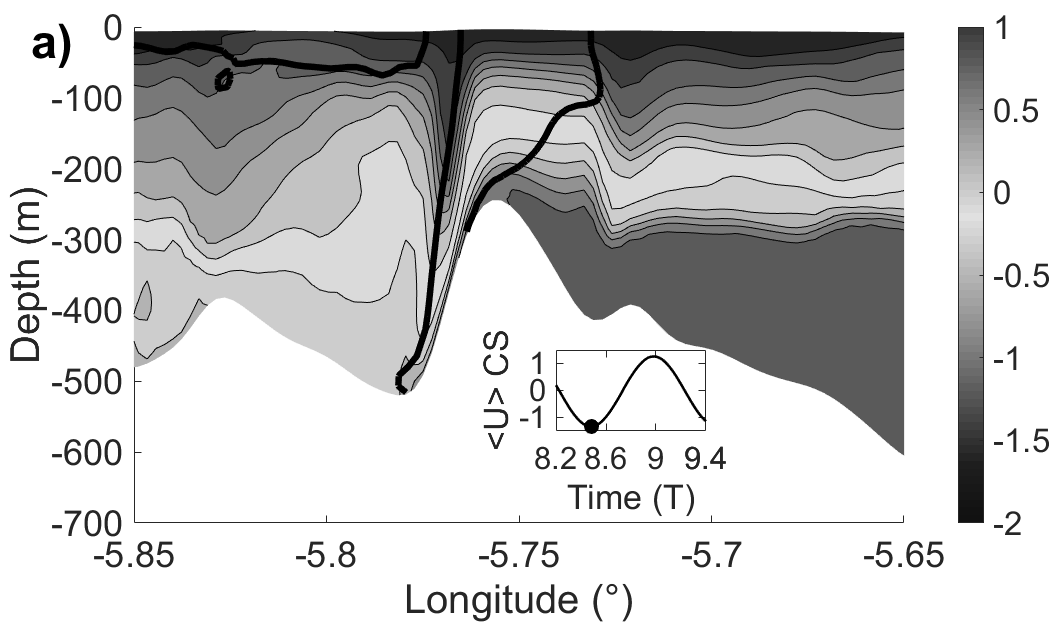
\includegraphics[width=1\textwidth]{./papier2D/RW_j4_9h12_spring.png}
  \end{subfigure}
  ~
    \centering
  \begin{subfigure}{0.45\linewidth}
  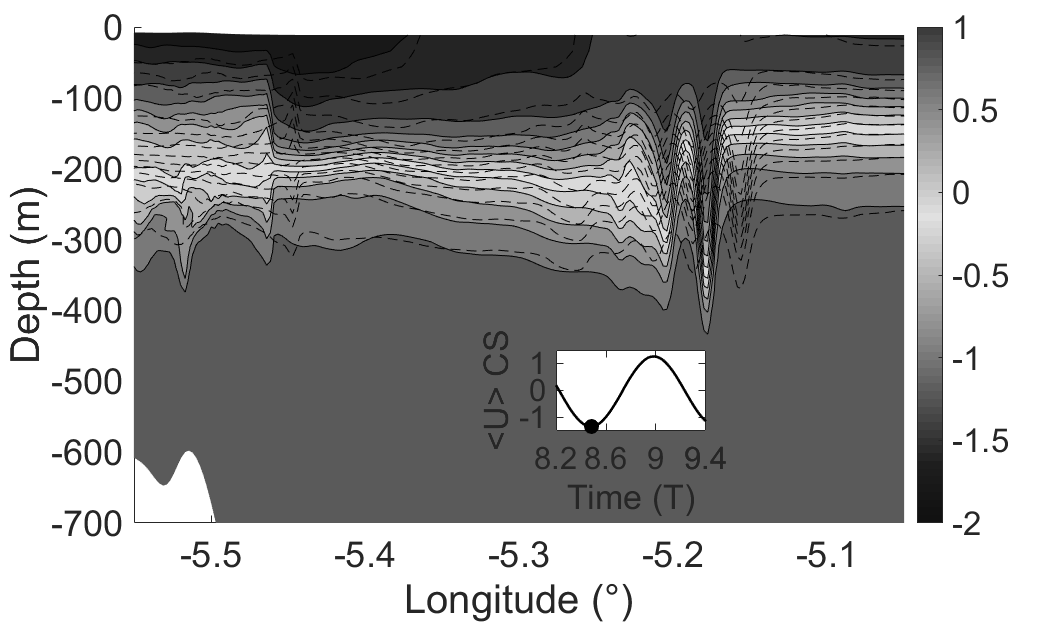
\includegraphics[width=1\textwidth]{./papier2D/CV_train_spring.png}
  \end{subfigure}
  \caption{Relative density contours in \textbf{SimB}.(a) area of F>1 (bolded contour). (b) Relative density contours in \textbf{SimRef}.}
  \label{fig_cv_spring}
\end{figure}


%%%%%%%%%%%%%%%%%%%%%%%%%%%%%%%%%%%%%%%%%%%%%%%%%%%%%%%%%%%%%%%%%%%%%%%%%%%%%
\subsection{Sensitivity to numerical factors}
%%%%%%%%%%%%%%%%%%%%%%%%%%%%%%%%%%%%%%%%%%%%%%%%%%%%%%%%%%%%%%%%%%%%%%%%%%%%%

\paragraph{The spatial resolution}% ($200 \rightarrow 50 m$)}
\label{TestNum}

\begin{figure}[!t]
   
   \centering
  \begin{subfigure}{0.5\linewidth}
  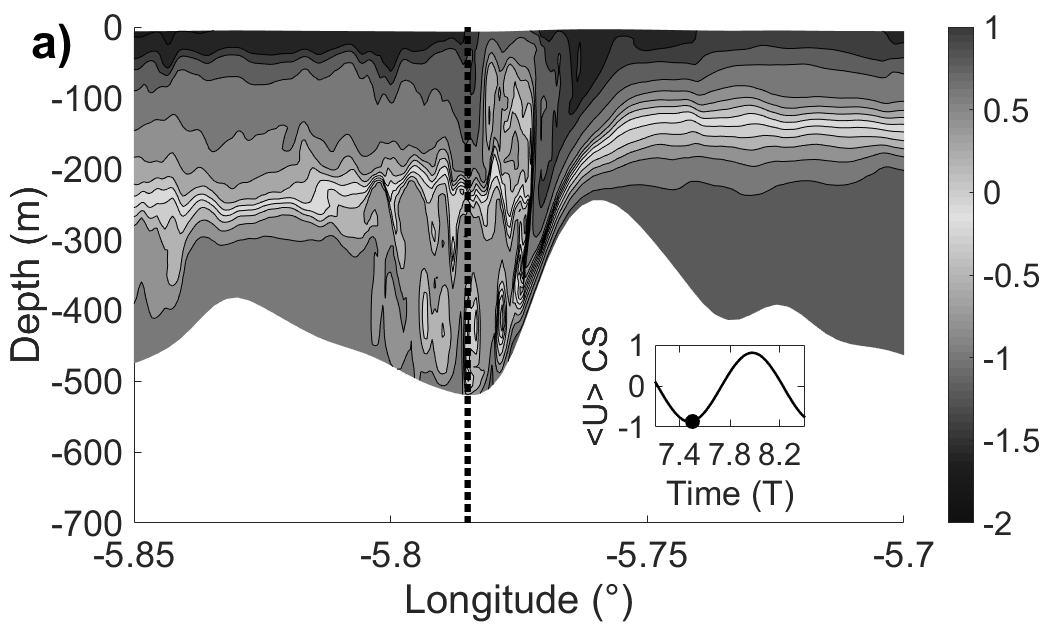
\includegraphics[width=\textwidth]{./papier2D/RW_J3_21h_50mtvd.png}
 % \subcaption{}
  \end{subfigure}
  ~
  \begin{subfigure}{0.5\linewidth}
  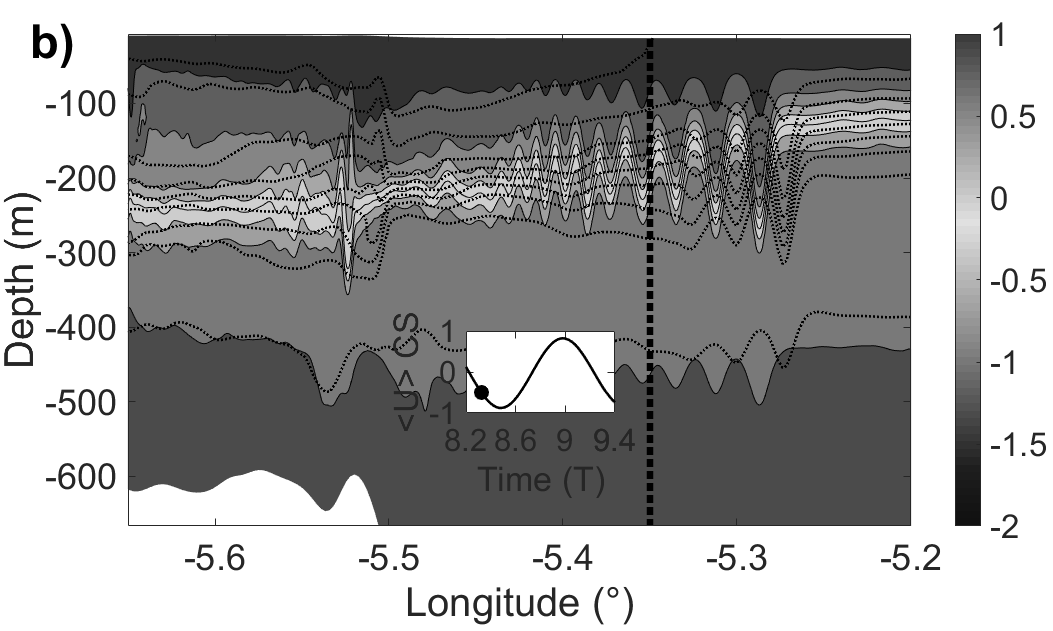
\includegraphics[width=\textwidth]{./papier2D/RW_J4_7h15train_50mtvd.png}
  %  \subcaption{}
  \end{subfigure}
  
  \begin{subfigure}{1\linewidth}
  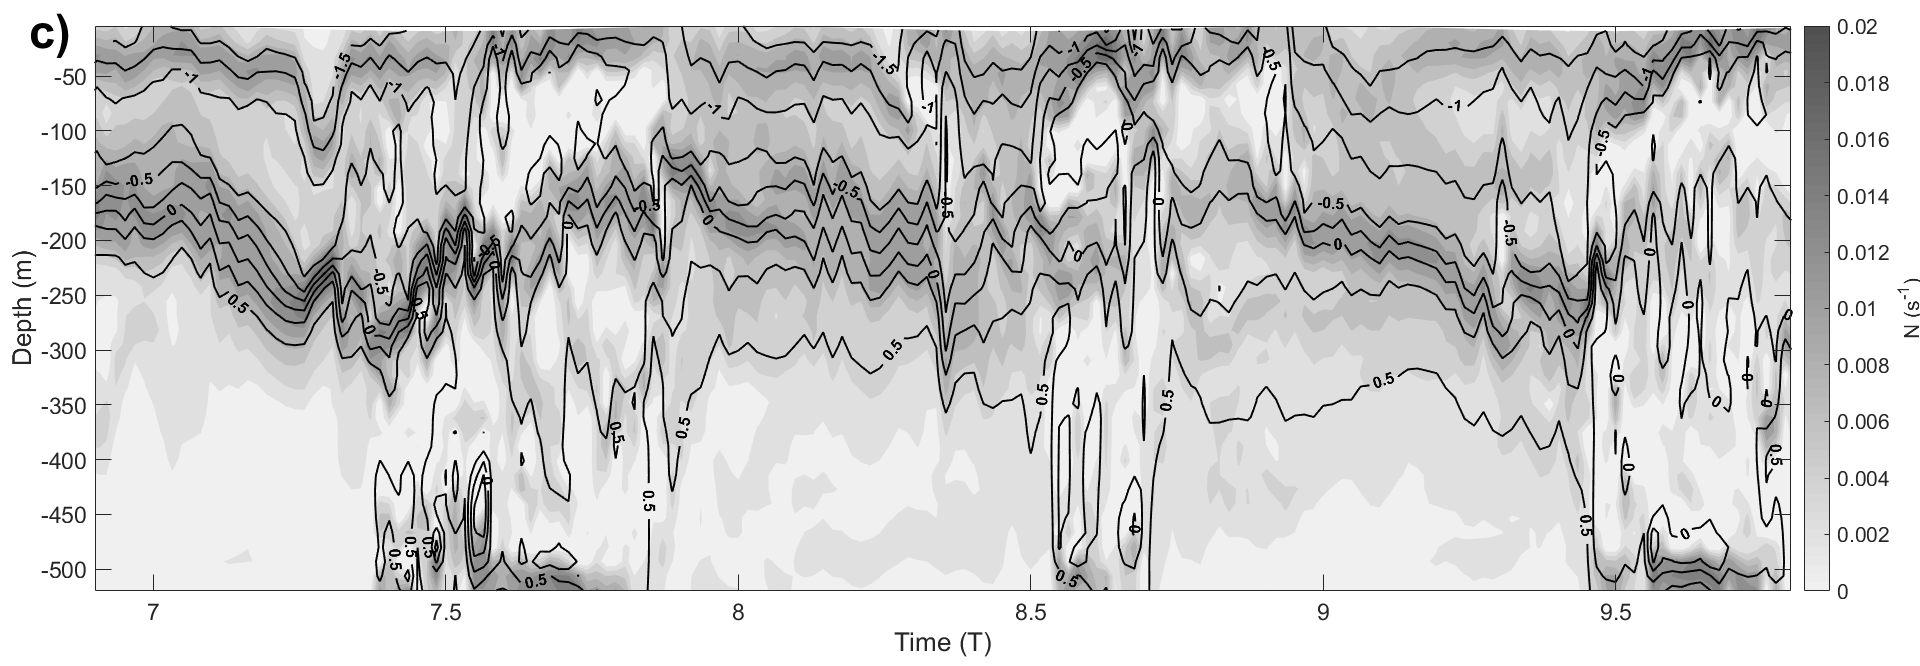
\includegraphics[width=\textwidth]{./papier2D/NrhoTZ_50mNH_5785.png}
  %  \subcaption{}
  \end{subfigure}
     
  \begin{subfigure}{1\linewidth}
  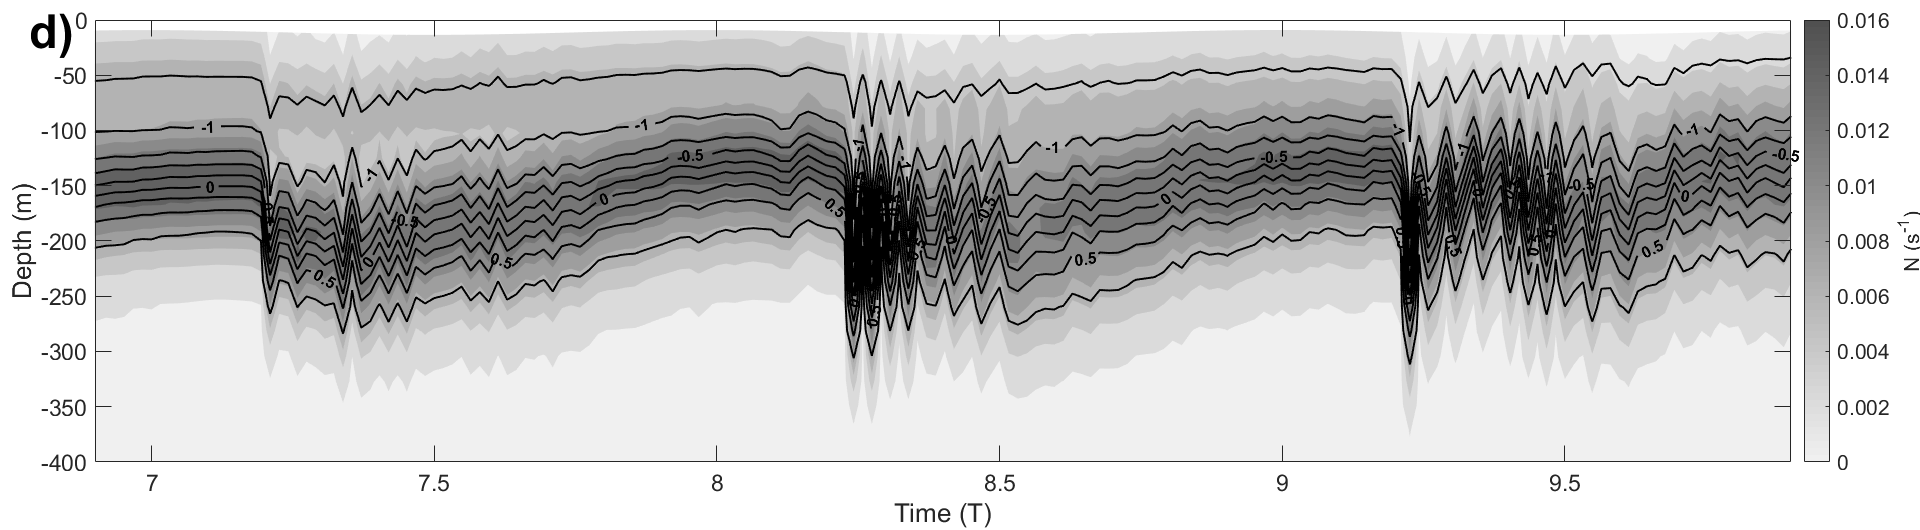
\includegraphics[width=\textwidth]{./papier2D/NrhoTZ_50mNH_535.png}
  %\subcaption{}
  \end{subfigure}
  \caption{(a) and (b) fields of relative density in configuration \textbf{Sim01}. (c) and (d) evolution of the profiles of relative density and $N$ in the water column at the positions of the dashed vertical lines in respectively (a) and (b). (b) dahsed lines are the correponding isopynals for configuration \textbf{SimRef}.}
  \label{fig50mtvd}
\end{figure}

 
% \begin{figure}[!h]
%  \begin{subfigure}{1\linewidth}
%   \includegraphics[width=\textwidth]{NTZrho_ref_5785.png}
%   %\subcaption{}
%   \end{subfigure}
  
%   \begin{subfigure}{1\linewidth}
%   \includegraphics[width=\textwidth]{NTZrho_ref_535.png}
%  % \subcaption{}
%   \end{subfigure}
%   \caption{\textbf{SimRef}}
%   \label{fig220NH}
% \end{figure}
 
A new configuration, \textbf{Sim01}, is investigated. It is identical to \textbf{SimRef} except for the resolution (now $\Delta x = 50\ m$) and time-steps are consequently adapted: $\Delta t_s = 1\ s$ and $\Delta t_f = 1/8\ s$. 

The initial stratification, the (volume) transport through CS and the location of the hydraulic controls (in the neighborhood of CS) are similar (not shown). The initial stratification is also close to the one in configuration \textbf{SimRef}.

Figures \ref{fig50mtvd}.a and \ref{fig50mtvd}.b show isopycnal fields at respectively $t = 7.5\ T$ and $t = 8.3\ T$. Figure \ref{fig50mtvd}.a is a close up on CS and on the hydraulic jump, whereas figure \ref{fig50mtvd}.b focuses on the resulting mode-1 ISW propagating in the deepest part of TN. In figure \ref{fig50mtvd}.b the dashed isocontours indicate the corresponding density field at the same time in the less resolved configuration \textbf{SimRef}. On both figures are featured vertical dashed lines. They indicate the location where the density profile of the water column is extracted to study its evolution in figure \ref{fig50mtvd}.c and \ref{fig50mtvd}.d, as well as the evolution of the Brunt-Väisälä frequency $N$,  given by:
\begin{equation}
N=\sqrt{ - \frac{g}{\rho_0} \frac{\partial \rho}{\partial z}}
\label{eqN}
\end{equation}

%The same evolution of the profile of $N$ at the same positions as for figures \ref{fig50mtvd}.c and \ref{fig50mtvd}.d is plotted in figures \ref{fig220NH}.a and \ref{fig220NH}.b for \textbf{SimRef}. 

A close comparison of figures \ref{CV_ressaut}.a and \ref{fig50mtvd}.a shows that the enhanced resolution allows the explicit modeling of billows west of CS. The comparison of the superimposed fields in \ref{fig50mtvd}.b shows that the mode-1 ISW waves are of comparable amplitude, but the ISW is slower in \textbf{Sim01} with additional waves in the train. Likewise, the mode-2 internal wave is slower in \textbf{Sim01}, and has additional mode-2 waves following it. The pycnocline in figure \ref{fig50mtvd}.d % and \ref{fig220NH}.b 
corresponds to areas where $N$ is large. It is slightly more stratified in \textbf{SimRef} (not shown). It can also be noted that for a same configuration, two consecutive mode-1 trains differ when comparing the number of waves per train.

%In figure \ref{fig220NH}.a, the isopycnal  $\rho' = 0.5\ kg/m^3$ is really deep or even absent in \textbf{SimRef} whereas it is at the bottom of the pycnocline in figure \ref{fig50mtvd}.c (\textbf{Sim01}). 
The lower layer is denser in \textbf{Sim01} than in \textbf{SimRef}. If we look at the other isopycnals, especially in the more stratified zones, there are numerous low-amplitude waves simulated in \textbf{Sim01} that are not present in \textbf{SimRef}, we can also see the signature of the billows as concentric ovals in figure \ref{fig50mtvd}.c. In this region, \textbf{Sim01} is more stratified than \textbf{SimRef}.

The increase in resolution does not change drastically the simulated processes. Indeed most characteristics (transport, speed of propagation, etc) are still of the same magnitude. One more prominent change is the modeling of billows in the hydraulic jump west of CS. An evaluation of the Richardson number (with $Ri =  N^2 / \left({\partial u}/{\partial z}\right)^2$, not shown) shows that $Ri < 1/4$ in the vicinity of the billows. Thus, this billows are potentially associated with Kelvin-Helmholtz instabilities, and linked to the beginning of the turbulent cascade. 
Stratification is deeply affected by the change in resolution, though attributing differences to the implicit dissipation of the numerical scheme or to the now explicitly modeled fine-scale instabilities, requires further sensitivity testing.
 
%%%%%%%%%%%%%%%
\paragraph{The non-hydrostatic algorithm}

\begin{figure}[!t]
  
  \begin{subfigure}{0.5\linewidth}
  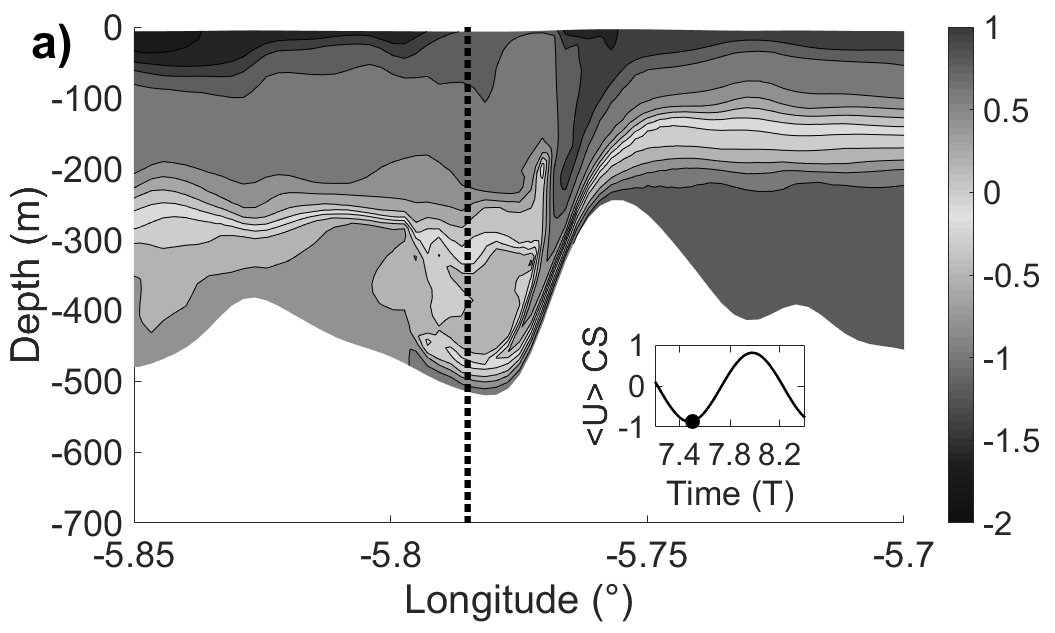
\includegraphics[width=\textwidth]{./papier2D/RW_J3_21_hydro.png}
  %\subcaption{}
  \end{subfigure}
  ~
  \begin{subfigure}{0.5\linewidth}
  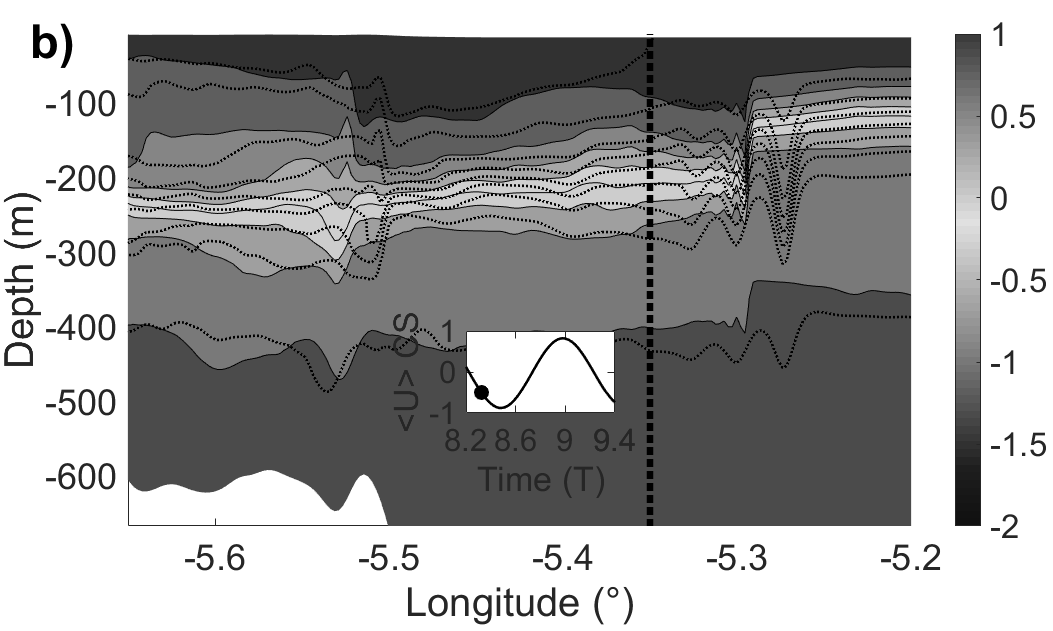
\includegraphics[width=\textwidth]{./papier2D/RW_83T_hydro.png}
  %\subcaption{}
  \end{subfigure}
 
%   \begin{subfigure}{1\linewidth}
%   \includegraphics[width=\textwidth]{Nrho_TZ_hydro_5785.png}
%   %\subcaption{}
%   \end{subfigure}
%   ~
%   \begin{subfigure}{1\linewidth}
%   \includegraphics[width=\textwidth]{Nrho_TZ_hydro_535.png}
%   %\subcaption{}
%   \end{subfigure}
  \caption{Same as figure \ref{fig50mtvd}.a %, b, c and d for configuration \textbf{Sim02}}
  and b for configuration \textbf{Sim02}}
  \label{fig220HNH}
\end{figure}

 Two simulations are now investigated with the hydrostatic version of CROCO. The first one, \textbf{Sim02}, is identical to \textbf{SimRef} (except that it is hydrostatic and its time-steps can be chosen larger: $\Delta t_s = 2\ s$ and $\Delta t_f = 1\ s$). The second one, \textbf{Sim03}, has a spatial resolution of $\Delta x = 50\ m$ and is identical to \textbf{Sim01} with this time two time-steps given by $\Delta t_s = 0.5\ s$ and $\Delta t_f = 0.25\ s$).

 Figure \ref{fig220HNH} %(\ref{figHH}) 
 is the same as figure \ref{fig50mtvd}% (\ref{fig220NH})
 for \textbf{Sim02}. The stratification and transports are equivalent in all simulations.
 
% \begin{figure}[!h]
%  \begin{subfigure}{1\linewidth}
%   \includegraphics[width=\textwidth]{NrhoTZ_50mH_5785.png}
%   %\subcaption{}
%   \end{subfigure}
  
%   \begin{subfigure}{1\linewidth}
%   \includegraphics[width=\textwidth]{NrhoTZ_50mH_535.png}
%  % \subcaption{}
%   \end{subfigure}
%   \caption{50m hydrostatique(\textbf{Sim03})}
%   \label{figHH}
% \end{figure}

 A very first difference, seen for example in figure \ref{fig220HNH}, is the form of the large-amplitude internal waves, that in \textbf{Sim02} is a single wave with a steepened front. This is due to the absence of non-hydrostatic dispersion which, as explained in subsection 3.2.1, induces energy transfers. Hence only non-linear steepening is effective and the waves in the hydrostatic simulations are not ISW. The resulting hydrostatic bore is slightly slower than the first wave of the train in \textbf{SimRef}. The hydraulic jump is similar in both configurations.
 
% Comparing the two hydrostatic configurations, \textbf{Sim02} and \textbf{Sim03}. The effect of this increased resolution are consistent with those in the previous subsection : in the better resolved case the internal bores are slightly slower, west of CS the $0.5\ kg/m^3$ isopycnal line is shallower. The bore in \textbf{Sim03} is steeper (not shown). Both east and west of CS, the 220-m resolved configuration (\textbf{Sim02}) is more stratified (higher values of $N$ are reached in the pycnocline), whereas this was the case only east of Camarinal Sill in the non-hydrostatic configuration.

\begin{figure}[!h]
  
  \begin{subfigure}{0.5\linewidth}
  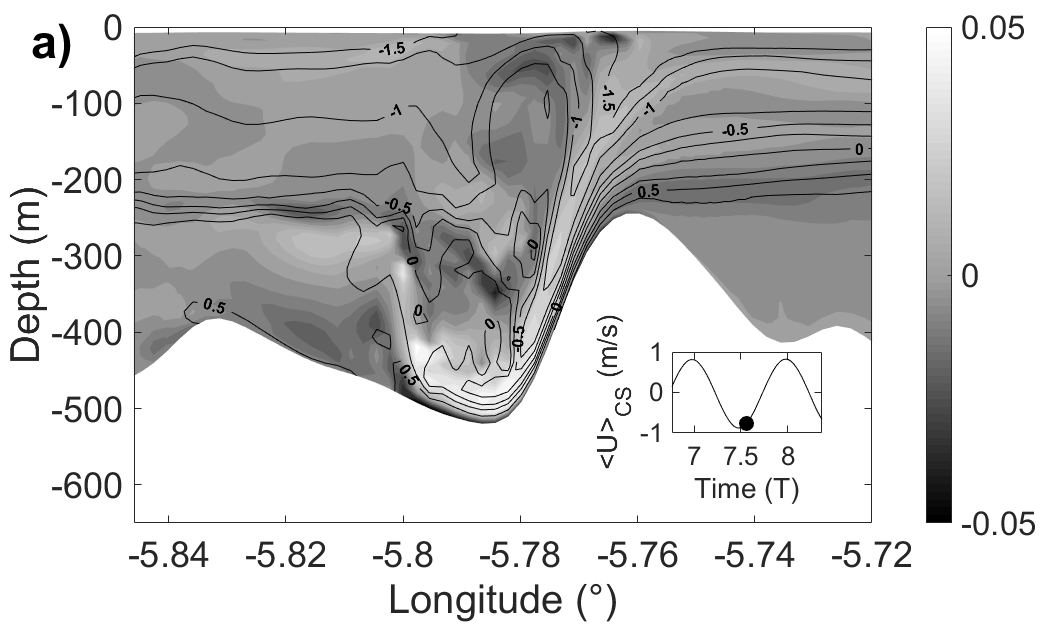
\includegraphics[width=\textwidth]{./papier2D/RV_75T_ref.png}
  %\subcaption{220m NH}
  \end{subfigure}
  ~
  \begin{subfigure}{0.5\linewidth}
  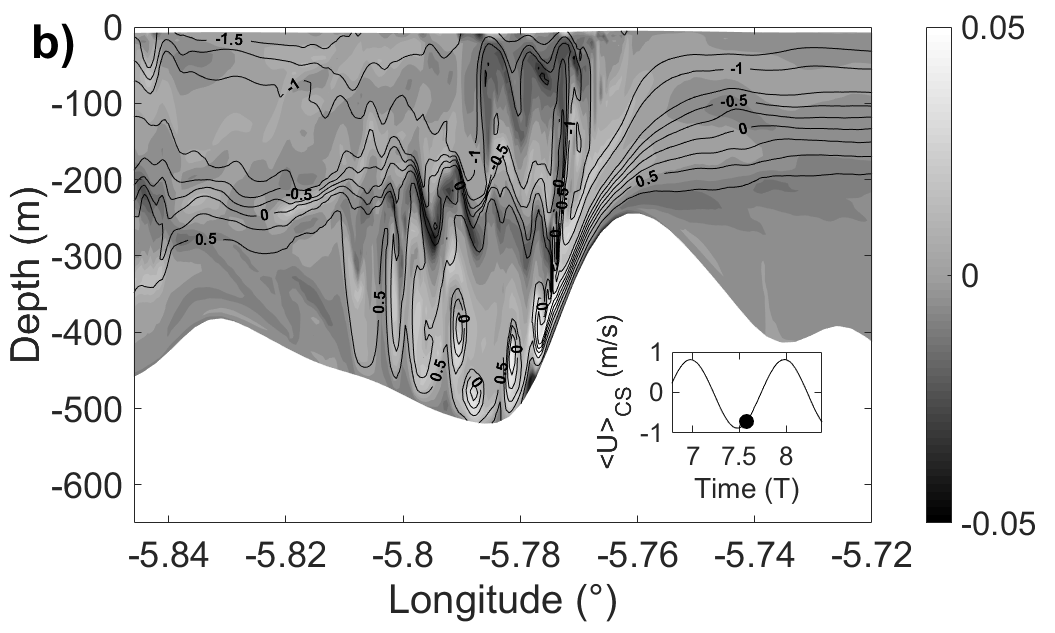
\includegraphics[width=\textwidth]{./papier2D/RV_75T_50m.png}
  %\subcaption{50m NH}
  \end{subfigure}
  
  \begin{subfigure}{0.5\linewidth}
  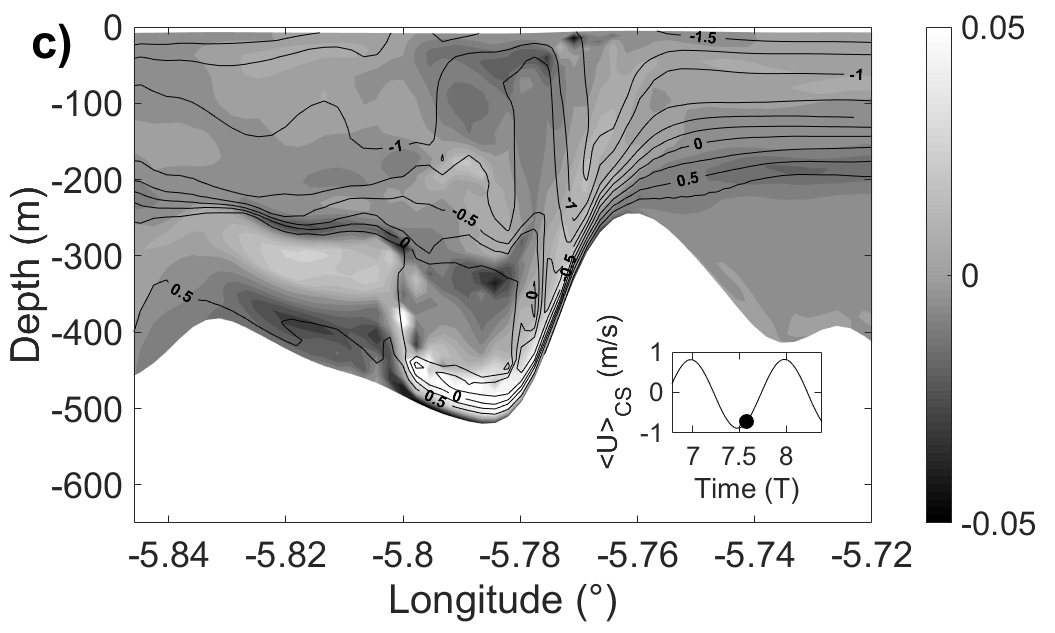
\includegraphics[width=\textwidth]{./papier2D/RV_75T_220mH.png}
  %\subcaption{220m H}
  \end{subfigure}
  ~
  \begin{subfigure}{0.5\linewidth}
  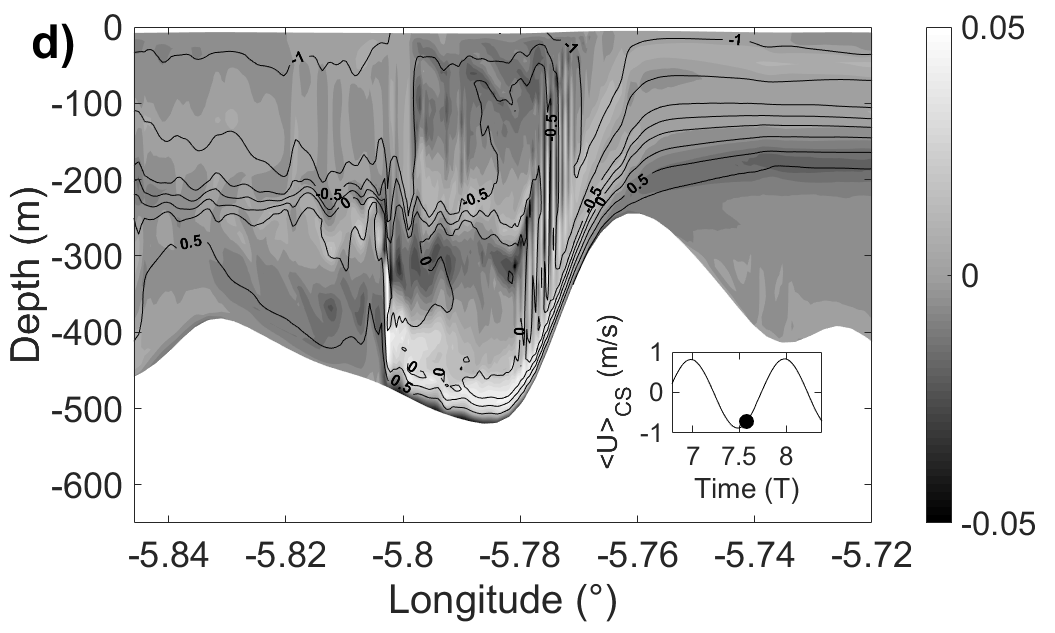
\includegraphics[width=\textwidth]{./papier2D/RV_75T_50mH.png}
  %\subcaption{50m H}
  \end{subfigure}
  \caption{XZ-Vorticity (s$^{-1}$) and isopycnals (kg/m$^3$) for \textbf{SimRef} (a, 220 m non-hydrostatic), \textbf{Sim01} (b, 50 m non-hydrostatic), \textbf{Sim02} (c, 220 m hydrostatic) and \textbf{Sim03} (d, 50 m hydrostatic)}
  \label{figvortCS}
\end{figure}

The same figure as figure \ref{fig220HNH} can be plotted for \textbf{Sim03} (not shown). Comparing the two hydrostatic configurations, \textbf{Sim02} and \textbf{Sim03}. The effect of this increased resolution are consistent with those in the previous subsection : in the better resolved case the internal bores are slightly slower, west of CS the $0.5\ kg/m^3$ isopycnal line is shallower. The wave in \textbf{Sim03} is steeper (not shown). Both east and west of CS, the 220-m resolved configuration (\textbf{Sim02}) is more stratified (higher values of $N$ are reached in the pycnocline), whereas this was the case only east of Camarinal Sill in the non-hydrostatic configuration.

The two 50 m-resolved configurations \textbf{Sim01} (non-hydrostatic) and \textbf{Sim03} (hydrostatic) show different large-amplitude waves and the differences are similar as between the less resolved \textbf{SimRef} and \textbf{Sim02}. However, the effect on stratification seems more visible as the eastern and western parts of CS \textbf{Sim01} are more stratified. A main difference is that the Kelvin-Helmholtz instabilities west of Camarinal Sill, and so the onset of the 2D-turbulent cascade, are only explicitly simulated in \textbf{Sim01}.
The increase in spatial resolution alone is not sufficient to solve the primal instabilities. This requires the implementation of the non-hydrostatic kernel and well-adapted numerical schemes for advection and dissipation (which are indicated in table \ref{tabsimref}).
 
An interesting consequence is that the vorticity balance is well simulated along the x and z-axis in the present vertical subsection. The fields of vorticity in the x-z plane during the outflow at CS are presented in figure \ref{figvortCS} for the four configurations \textbf{SimRef}, \textbf{Sim01}, \textbf{Sim02} and \textbf{Sim03}. In all configurations, positive vorticity structures can be seen associated with the shear of the Mediterranean outflow. In configuration \textbf{SimRef} and the two hydrostatic ones (figures \ref{figvortCS}.a, \ref{figvortCS}.c and \ref{figvortCS}.d), the positive vorticity structure near the bottom is 3-km long and $\approx$ 50-m high, whereas for \textbf{Sim01} (figure \ref{figvortCS}.b) multiple structures of $\approx$ 150-m diameter are visible (the Kelvin-Helmotz instabilities).
 
Mixing is different in all four configurations \textbf{SimRef}, \textbf{Sim01}, \textbf{Sim02} and \textbf{Sim03}, with impact  both of enhanced resolution, and of the combination of enhanced resolution and non-hydrostatic code. However, in less resolved simulation the switch between hydrostatic and non-hydrostatic configuration has a lesser impact.


%%%%%%%%%%%%%%%%%%%%%%%%%%%%%%%%%%%%%%%%%%%%%%%%%%%%%%%%%%%%%%%%
%%%%%%%%%%%%%%%%%%%%%%%%%%%%%%%%%%%%%%%%%%%%%%%%%%%%%%%%%%%%%%%%
%    Rapport intermédiaire de Lucie
%%%%%%%%%%%%%%%%%%%%%%%%%%%%%%%%%%%%%%%%%%%%%%%%%%%%%%%%%%%%%%%%
%%%%%%%%%%%%%%%%%%%%%%%%%%%%%%%%%%%%%%%%%%%%%%%%%%%%%%%%%%%%%%%%

\paragraph{Sensibilité aux schémas d'advection}

\noindent \textit{Cette sous-section, en français est basée sur le rapport intermédiaire $T_0 + 12$ mois écrit par Lucie Bordois, post-doctorante au laboratoire d'Aérologie.}\\

Afin d'évaluer l'impact des schémas d'advection dans la maquette \textbf{SimRef}, une première simulation de référence est réalisée à partir d'un schéma d’advection verticale \textit{« Splines»} (respectivement \textit{« Akima »)} pour la quantité de mouvement (respectivement les traceurs). Ces schémas sont classiquement utilisés dans les maquettes CROCO en version hydrostatique pour des simulations régionales ou côtières.\\
La section verticale 2D (Figure \ref{Fig_TVD1}) montre des oscillations sur les champs de traceurs et de vitesses dans les zones de forts cisaillements verticaux (particulièrement visibles au-dessus de CS durant la phase d’initialisation \textit{« lock-exchange »}. 

%%%%%%%%%%%%%%%%%%%% Figure/Image No: 1 starts here %%%%%%%%%%%%%%%%%%%%

\begin{figure}[!h]
	\begin{Center}
		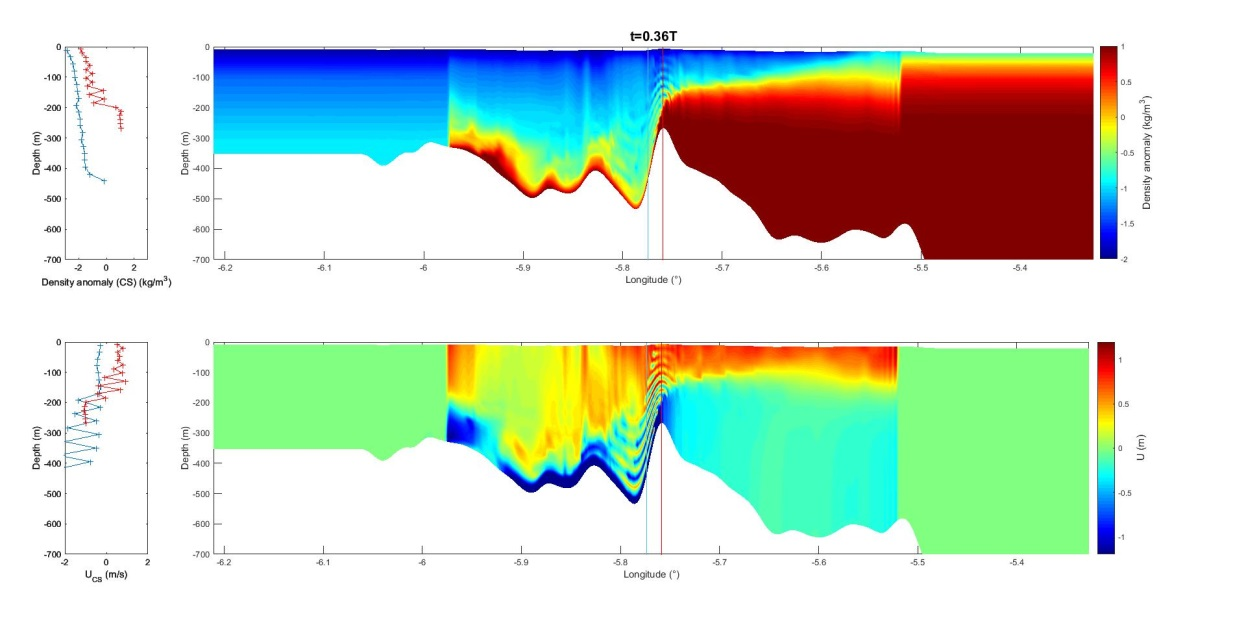
\includegraphics[width=5.66in,height=2.83in]{./media/TVD1.jpeg}
		\caption{ : Section verticale du champ de vitesse horizontale (doite-bas) et du champ d’anomalie de densité (droite-haut) à t=0.36 T (avec T la période de M2) durant la phase de spin-up (initialisation \textit{« lock-exchange »}) dans 2D. (Panneaux de gauche) Profil vertical situé au-dessus de Camarinal Sill (localisé par les lignes rouge et bleue sur les panneaux de droite).}
		\label{Fig_TVD1}
		%\label{fig:_Section_verticale_du_champ_de_vitesse_horizontale_doitebas_et_du_champ_danomalie_de_densit_droitehaut__t036T_T_reprsente_la_priode_de_M2_durant_la_phase_de_spinup_initialisation_Lockexchange_dans_2D_Panneaux_de_gauche_Profil_vertical_situ_audessus_de_Camarinal_Sill_localis_par_les_lignes_rouge_et_bleue_sur_les_panneaux_de_droite}
	\end{Center}
\end{figure}
%%%%%%%%%%%%%%%%%%%% Figure/Image No: 1 Ends here %%%%%%%%%%%%%%%%%%%%

Nous avons donc cherché à évaluer l'impact de différents schémas numériques d’advection et de dissipation turbulente sur ces instabilités numériques. 

\noindent La Figure (\ref{Fig_TVD2} – haut) montre qu'en version 2D-verticale, l’utilisation d’un schéma d’advection de type WENO d’ordre 5 sur la verticale pour les traceurs permet de supprimer l’apparition d’instabilités numériques sur les champs de traceurs. Cependant, les instabilités numériques persistent dans ce cas sur les champs de vitesse (Figure \ref{Fig_TVD2} – bas). Ce résultat montre la nécessité pour la communauté CROCO de disposer de schémas d’advection verticale monotone (type TVD) ou quasi-monotone (type WENO) pour la quantité de mouvement (U, V en hydrostatique et W en version non-hydrostatique). 

%%%%%%%%%%%%%%%%%%%% Figure/Image No: 2 starts here %%%%%%%%%%%%%%%%%%%%
\begin{figure}[!h]
	\begin{Center}
		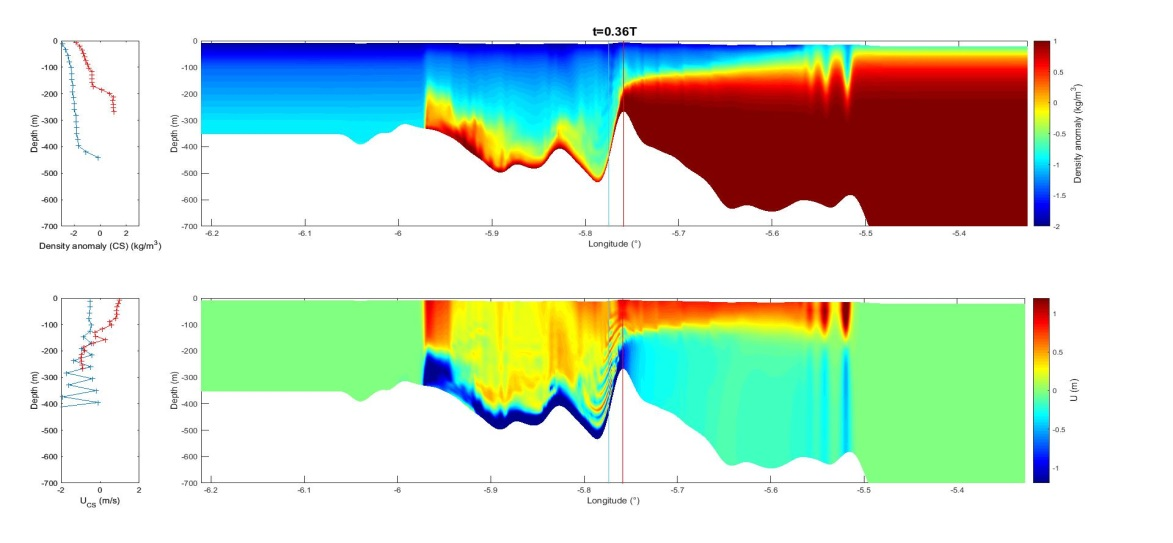
\includegraphics[width=4.98in,height=2.35in]{./media/TVD2.jpeg}
		\caption{ : Section verticale du champ de vitesse horizontale (doite-bas) et du champ d’anomalie de densité (droite-haut) à t=0.36 T durant la phase de spin-up (initialisation « Lock-Exchange ») dans 2DTS-WENO5. (Panneaux de gauche) Profil vertical situé\  au-dessus de Camarinal Sill (localisé par les lignes rouge et bleue sur les panneaux de droite).}
		\label{Fig_TVD2}
		%\label{fig:_Section_verticale_du_champ_de_vitesse_horizontale_doitebas_et_du_champ_danomalie_de_densit_droitehaut__t036T_durant_la_phase_de_spinup_initialisation_LockExchange_dans_2DTSWENO5_Panneaux_de_gauche_Profil_vertical_situ__audessus_de_Camarinal_Sill_localis_par_les_lignes_rouge_et_bleue_sur_les_panneaux_de_droite}
	\end{Center}
\end{figure}

%%%%%%%%%%%%%%%%%%%% Figure/Image No: 2 Ends here %%%%%%%%%%%%%%%%%%%%
\noindent Des schémas d’advection TVD ont été codés par l'équipe de développement CROCO et ont ainsi été testés et comparés dans le cadre du présent contrat. La Figure \ref{Fig_TVD3} (bas) présente un premier résultat montrant la disparition des oscillations lorsqu’un tel schéma est utilisé pour l’advection verticale des composantes horizontales de la quantité de mouvement. La contre-partie anticipable est une augmentation locale de la dissipation liée à l'utilisation du schéma TVD.

%%%%%%%%%%%%%%%%%%%% Figure/Image No: 3 starts here %%%%%%%%%%%%%%%%%%%%

\begin{figure}[!h]
	\begin{Center}
		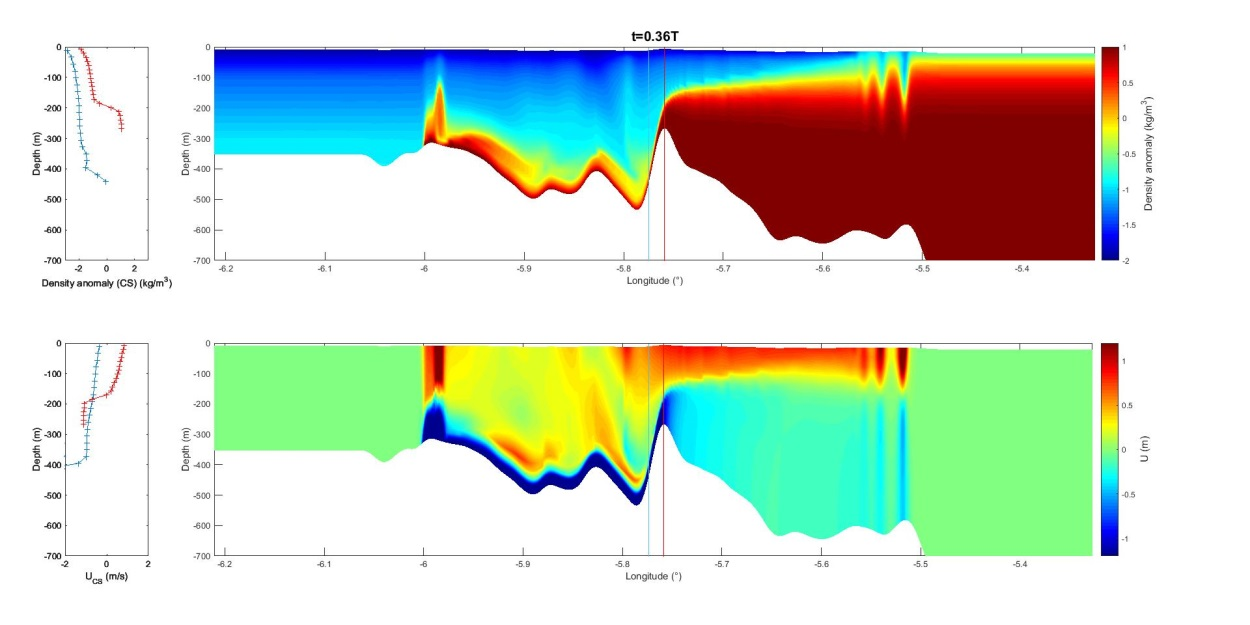
\includegraphics[width=5.68in,height=2.84in]{./media/TVD3.jpeg}
		\caption{: Section verticale du champ de vitesse horizontale (doite-bas) et du champ d’anomalie de densité (droite-haut) à t=0.36 T durant la phase de spin-up (initialisation « Lock-exchange ») dans 2DTS-WENO5,UV-TVD. (Panneaux de gauche) Profil vertical situé au dessus de Camarinal Sill (localisé par les lignes rouge et bleue sur les panneaux de droite).}
		\label{Fig_TVD3}
		%\label{fig:_Section_verticale_du_champ_de_vitesse_horizontale_doitebas_et_du_champ_danomalie_de_densit_droitehaut__t036T_durant_la_phase_de_spinup_initialisation_Lockexchange_dans_2DTSWENO5UVTVD_Panneaux_de_gauche_Profil_vertical_situ_au_dessus_de_Camarinal_Sill_localis_par_les_lignes_rouge_et_bleue_sur_les_panneaux_de_droite}
	\end{Center}
\end{figure}
%%%%%%%%%%%%%%%%%%%% Figure/Image No: 3 Ends here %%%%%%%%%%%%%%%%%%%%

\noindent Les premiers résultats obtenus avec les schémas d’advection de type TVD et WENO confirment un certain nombre de choix numériques assez fondamentaux de la communauté CROCO concernant l’utilisation de schémas numériques « monotones » ou « quasi-monotones ». Les tests de sensibilité réalisés dans le cadre de la présente étude ont de plus montré qu’il était possible de supprimer les oscillations numériques obtenus avec des schémas numériques non monotones plus classiques mais en ayant recours à une dissipation numérique jugée trop importante (coefficient de mélange vertical > 0.001 m²/s $\&$  coefficient de viscosité $ \geq $ 0.1 m²/s) et en tout cas incompatible avec la simulation des trains de solitons observés en aval du détroit (dissipation numérique des trains d’ondes : sous-estimation de l’amplitude des solitons et de leur zone de propagation). Nous avons choisi de ne pas privilégier, dans un premier temps tout au moins, l’implémentation ou l’évaluation de techniques plus sophistiquées pour la modélisation des processus sous-maille et la modélisation des fronts, nous orientant vers des schémas numériques monotones d’advection jugés plus « physiques » et offrant de meilleurs résultats numériques. Ces schémas monotones ne nécessitant pas de schémas de dissipation turbulence numérique additionnels permettent la réalisation de simulation à haute résolution dites MILES pour \textit{(pour Monotone Implicit Large Eddy Simulation)}.\\

\noindent Suite à l’observation dans la simulation 2DV d’oscillations numériques dans les zones de forts cisaillements de vitesse, des schémas d’advection TVD pour l’advection verticale et horizontale des composantes horizontales (U-V) et verticale (W) de la quantité de mouvement ont été implémentés dans le modèle CROCO. Ces schémas ont été codés avec différentes options de limiteurs plus ou moins diffusifs \textit{(MINMOD, VanLeer, SUPERBEE)}. Nous avons évalué l’impact de ces nouveaux schémas numériques d’advection sur les champs de vitesse horizontale de la simulation 3D NH-REF. La Figure \ref{Fig_TVD4} présente des résultats très encourageants: l’utilisation de ces schémas permet de supprimer totalement l’apparition d’instabilités numériques sur les champs de vitesses horizontales au-dessus des reliefs abruptes (figures \ref{Fig_TVD4} du milieu et du bas) avec des conséquences tout à fait acceptables sur la dissipation implicite.

%%%%%%%%%%%%%%%%%%%% Figure/Image No: 4 starts here %%%%%%%%%%%%%%%%%%%%

\begin{figure}[!h]
	\begin{Center}
		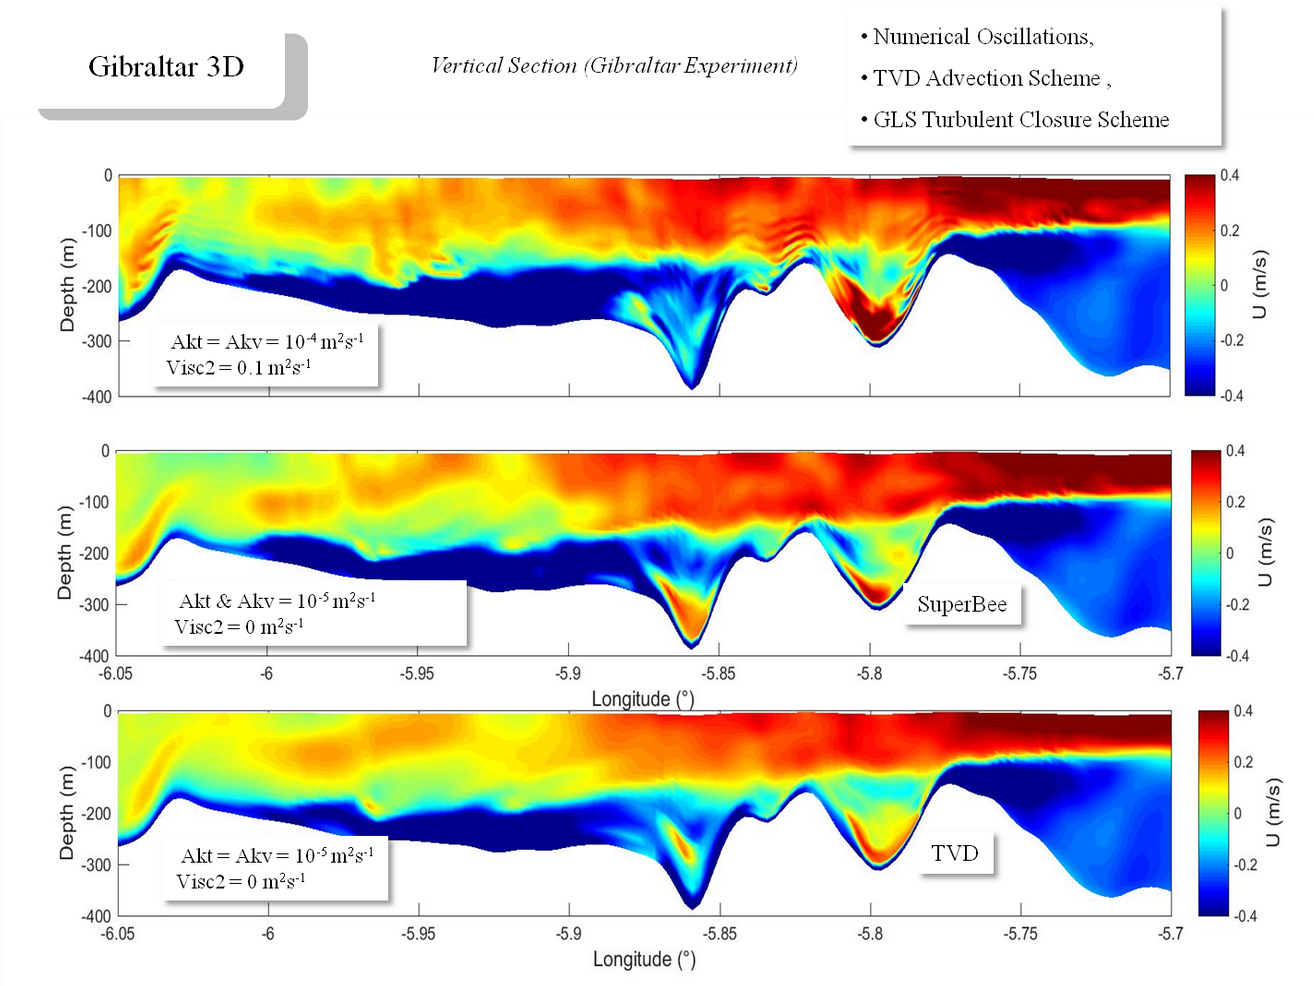
\includegraphics[width=6.29in,height=3.55in]{./media/TVD4.png}
		\caption{ : Test de sensibilité du champ de vitesse horizontale aux schémas d’advection de la quantité de mouvement. (haut) Section verticale du champ de vitesse horizontale à t=1.36T dans la maquette 3DUP3-SPLINES. (milieu) Section verticale du champ de vitesse horizontale à t=1.36 T dans la maquette 3DTVD-SUPERBEE. (bas) Section verticale du champ de vitesse horizontale à t=1.36T dans la maquette 3DTVD-MINMOD.}
		\label{Fig_TVD4}
		%\label{fig:_Test_de_sensibilit_du_champ_de_vitesse_horizontale_aux_schmas_dadvection_de_la_quantit_de_mouvement_haut_Section_verticale_du_champ_de_vitesse_horizontale__t136T_dans_la_maquette_3DUP3SPLINES_milieu_Section_verticale_du_champ_de_vitesse_horizontale__t136T_dans_la_maquette_3DTVDSUPERBEE_bas_Section_verticale_du_champ_de_vitesse_horizontale__t136T_dans_la_maquette_3DTVDMINMOD}
	\end{Center}
\end{figure}


%%%%%%%%%%%%%%%%%%%% Figure/Image No: 4 Ends here %%%%%%%%%%%%%%%%%%%%

\par

\par

\begin{justify}
Anticipant sur la section (\ref{section3DNHREF}) dédiée à la maquette NH-REF et par soucis de cohérence, nous évaluons maintenant l’impact de ces nouveaux schémas numériques sur la propagation des trains d’ondes solitaires dans la simulation 3D-NH REF : sur la Figure \ref{Fig_TVD5}, on observe que les schémas d’advection de type TVD (MINMOD, VanLeer $\&$  SUPERBEE) ont tendance à dissiper un peu plus les ondes solitaires que les schémas d’advection UP3 et SPLINES (amplitude et vitesse verticale associé aux solitons plus faibles). Cependant, l’utilisation du limiteur SUPERBEE permet de réduire significativement ces effets dissipatifs. Une nouvelle version des schémas d’advection TVD moins dissipative est actuellement en développement.
\end{justify}\par


%%%%%%%%%%%%%%%%%%%% Figure/Image No: 5 starts here %%%%%%%%%%%%%%%%%%%%

\begin{figure}[!h]
	\begin{Center}
		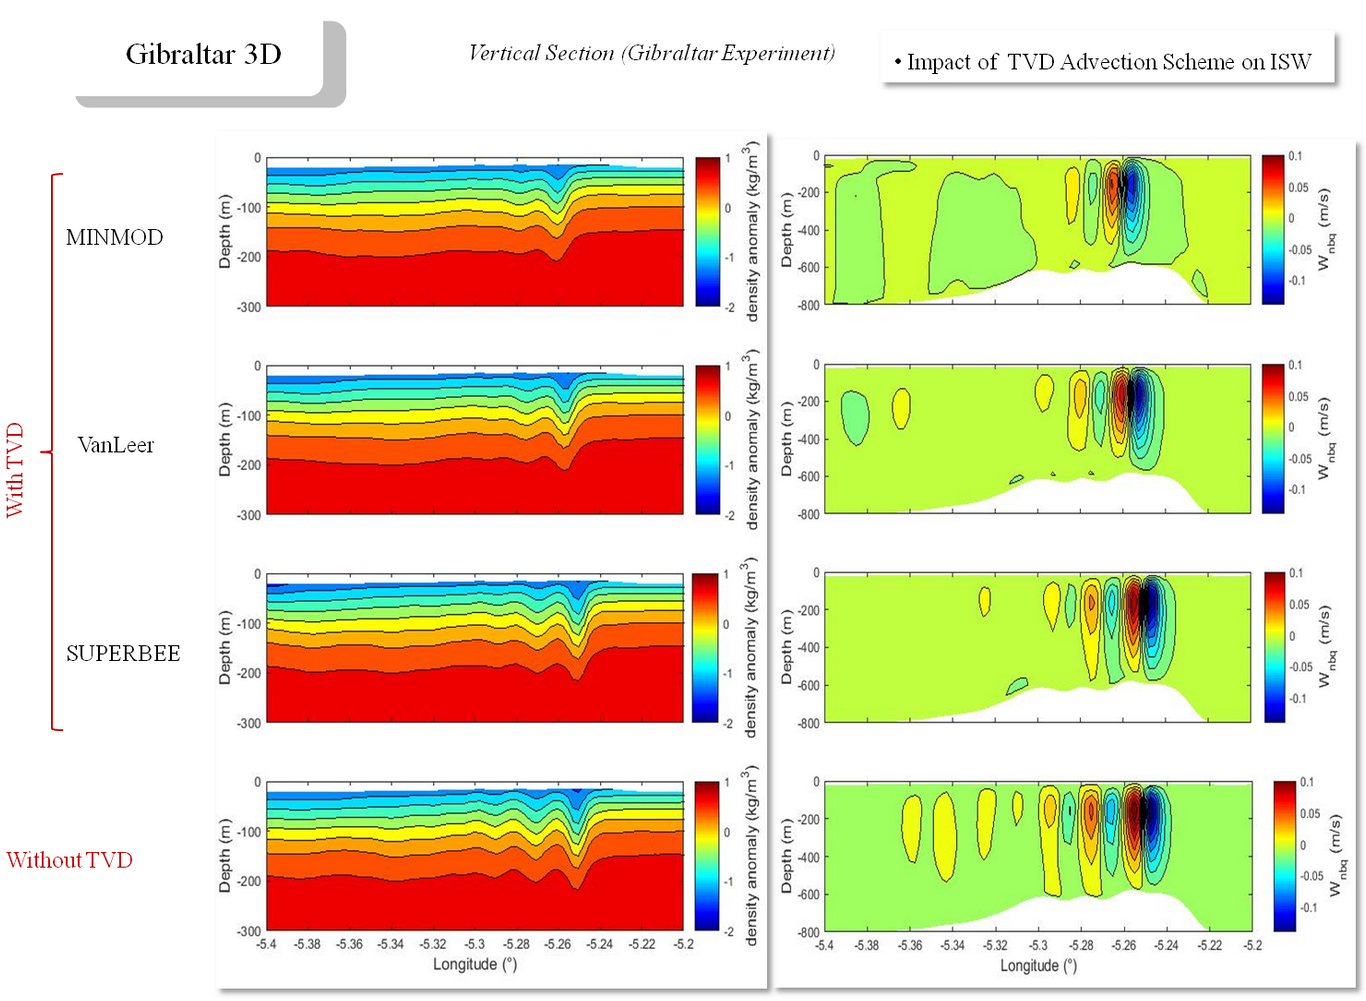
\includegraphics[width=6.3in,height=2.91in]{./media/TVD5.png}
		\caption{: Test de sensibilité des trains d’ondes solitaires aux schémas d’advection de la quantité de mouvement.\ \ \ \ \ \   Sections verticales des champs d’anomalie de densité et de vitesse verticale à t=1.1T : (a)  pour la maquette 3DTVD-MINMOD, (b) pour la maquette 3DTVD-VanLeer,\  (c)  pour la maquette 3DTVD-SUPERBEE, (d) pour la maquette 3DUP3-SPLINES.}
		\label{Fig_TVD5}
		%\label{fig:_Test_de_sensibilit_des_trains_dondes_solitaires_aux_schmas_dadvection_de_la_quantit_de_mouvement________Sections_verticales_des_champs_danomalie_de_densit_et_de_vitesse_verticale__t11T_a__pour_la_maquette_3DTVDMINMOD_b_pour_la_maquette_3DTVDVanLeer__c__pour_la_maquette_3DTVDSUPERBEE_d_pour_la_maquette_3DUP3SPLINES}
	\end{Center}
\end{figure}


%%%%%%%%%%%%%%%%%%%% Figure/Image No: 5 Ends here %%%%%%%%%%%%%%%%%%%%


%%%%%%%%%%%%%%%%%%%%%%%%%%%%%%%%%%%%%%%%%%%%%%%%%%%%%%%%%%%%%%%%%%%%%%%%%%%%%
\subsection{Discussion and conclusion}
%%%%%%%%%%%%%%%%%%%%%%%%%%%%%%%%%%%%%%%%%%%%%%%%%%%%%%%%%%%%%%%%%%%%%%%%%%%%%


In the introduction of the present study, two objectives were originally set. A first one concerns the understanding of the small-scale dynamics of the strait of Gibraltar, the other is associated to the capacity of the new time-splitting regional model CROCO-NBQ to render an easy-to-implement forecast of such a dynamics. Both objectives have been pursued in parallel and several seminal results have been obtained.

The present study confirms that both the generation of large-amplitude mode-1 and mode-2 internal waves and the onset of turbulence and its energy cascade could be simulated in the strait of Gibraltar with reasonable accuracy based on a simple, computationally efficient vertical configuration. The characteristics of the simulated internal waves compare indeed well with published observations, with numerical studies and with KdV model for ISWs. Barotropic tides are propagated with an explicit free-surface model. The mechanisms of generation, propagation and advection of mode-1 and 2 internal waves have been detailed based on maps of criticality produced for the exchange flow.
 
 To do so, a new type of non-hydrostatic non-Boussinesq algorithm (Auclair et al., 2018) had to be implemented in the otherwise numerically-efficient ROMS-CROCO and the resulting (pseudo-) compressible time-splitting code was implemented for the very first time in a realistic configuration. Sensitivity tests confirmed that a non-hydrostic (here non-Boussinesq) kernel is required (i) to simulate ISW trains and (ii) to explicitly simulate the onset of the turbulence energy cascade when (in the present case) resolution is increased from approximately 200 m to 50 m. Such small-scale turbulent structures have for instance been observed at CS by Wesson et al. (1994), where they where associated to dissipation of $10^{-2}\ W/kg$. We reached the conclusion that resolutions finer than a few hundred meters have to be associated to a refinement of the physics of the numerical kernel of the ocean code from hydrostatic to non-hydrostatic.\\
 The way the vertical configuration can be built has also been detailed with a particular attention paid to the bathymetry (implicit representation of 3D effects around isolated mounts...) and to the representation of the Coriolis pseudo-force (implicit representation of the funneling effect in the strait...). The proposed approach can now easily be implemented in other regions of the world where for instance ISW or just internal waves need to be explicitly simulated, leading to numerically-efficient forecasting tools.
 
 Vertical 2D configurations are yet limited by the representation of the velocity shear between inflowing Atlantic Waters and outflowing Mediterranean waters and more generally by the bathymetry. The inclusion of restratification process (surface and boundary forcing) would allow the model to remain accurate for a greater number of tidal cycles. The chosen Lock-exchange-like initialization additionally requires a rather long spin-up period but it provides a simple strategy to initialize a configuration with crude information on the stratification. In the present case, only two vertical profiles of temperature and salinity are required (one per variable and per water mass).
 
 The absence of transverse effects in the strait could be at least partly simulated by re-considering the definition of Coriolis pseudo-force. However several remaining processes could not be taken into account: the transverse propagation of ISWs in the strait of Gibraltar (S\'anchez'Garrido et al., 2011 and Vlasenko et al., 2009) and furthermore in the Alboran Sea, the hydraulic control in TN (Farmer and Armi, 1988, Sannino et al., 2009) or the boiling-water over CS (Bruno et al., 2002), the reflexion onto the Moroccan coast... Only the ``onset'' of the turbulence cascade could be simulated based on primary Kelvin-Helmholtz instabities. The simulation of the following secondary instabilities and down the road, the resulting energy cascade as well as the long term impact on Mediterranean and North Atlantic circulation of the refined representation of the dynamics of the strait both require a fully 3D approach which is possible with CROCO-NBQ. 
 

% Shortcomings:
% \begin{itemize}
% \item{subsection must e in pivilged diection of propagation }
% \item{
%One limitation of our testing is the lock exchange initialization that uses profiles of two water masses depicted in figure \ref{fig_LEx}. In reality, more than one water mass enter the Strait of Gibraltar on both the Atlantic and Mediterranean side. On the Mediterranean side, water masses are intermediate waters such as LIW, and also deep waters formed by deep convection that can get sucked over the sill, whereas on the Atlantic side... The mixing of the different water masses affects biogeochemical transport to the eastern end of the Srait... (macias 2006) }
%\item{3D effects/phenomena absent : control in TN, 'boiling-water' in neap-tide, reflexion on Moroccan coast, etc...3D turbulent cascade }
%\item{no restratification process}
%\item{difficulty with velocity shear}
%\end{itemize}

 \color{black}

\clearpage
%%%%%%%%%%%%%%%%%%%%%%%%%%%%%%%%%%%%%%%%%%%%%%%%%%%%%%%%%%%%%%%%%%%%%%%%%%%%%
\subsection{Appendix : computation of a Froude number}
%%%%%%%%%%%%%%%%%%%%%%%%%%%%%%%%%%%%%%%%%%%%%%%%%%%%%%%%%%%%%%%%%%%%%%%%%%%%%
Froude number for the mode-n internal wave $F_n$ is defined as $F_n=U/c^*_n$ with c$^*_n$ the linear internal wave speed of the mode-n internal wave.
 $c^*_n=\omega / k_n = \sqrt{g'h}/n$
 where $\omega$ is the wave frequency, here the M2-tidal frequency, and 
\begin{equation}
\label{eqK}
k_n=\pm \frac{n \pi}{H} \left( \frac{\omega^2 - f^2}{N^2 - \omega^2} \right) ^{1/2} 
\end{equation}

This expression of k$_n$ is derived from the linear propagation equation (Gill, 1982) derived from the Navier-Stokes conservation of momentum equations (see subsection \ref{NavierStokes}):
\begin{equation}
 W'' + k^2 \frac{N^2 - \omega^2}{\omega ^2 - f^2}W = 0
\end{equation}
with bottom and surface boundary conditions $w(0) = 0$ and $w(-H) = 0$. This expression of W$_n$ gives the structures of the vertical modes. N is chosen as the average stratification of the water column and its expression is given by equation (\ref{eqN}). 

\begin{figure}[!h]
\centering
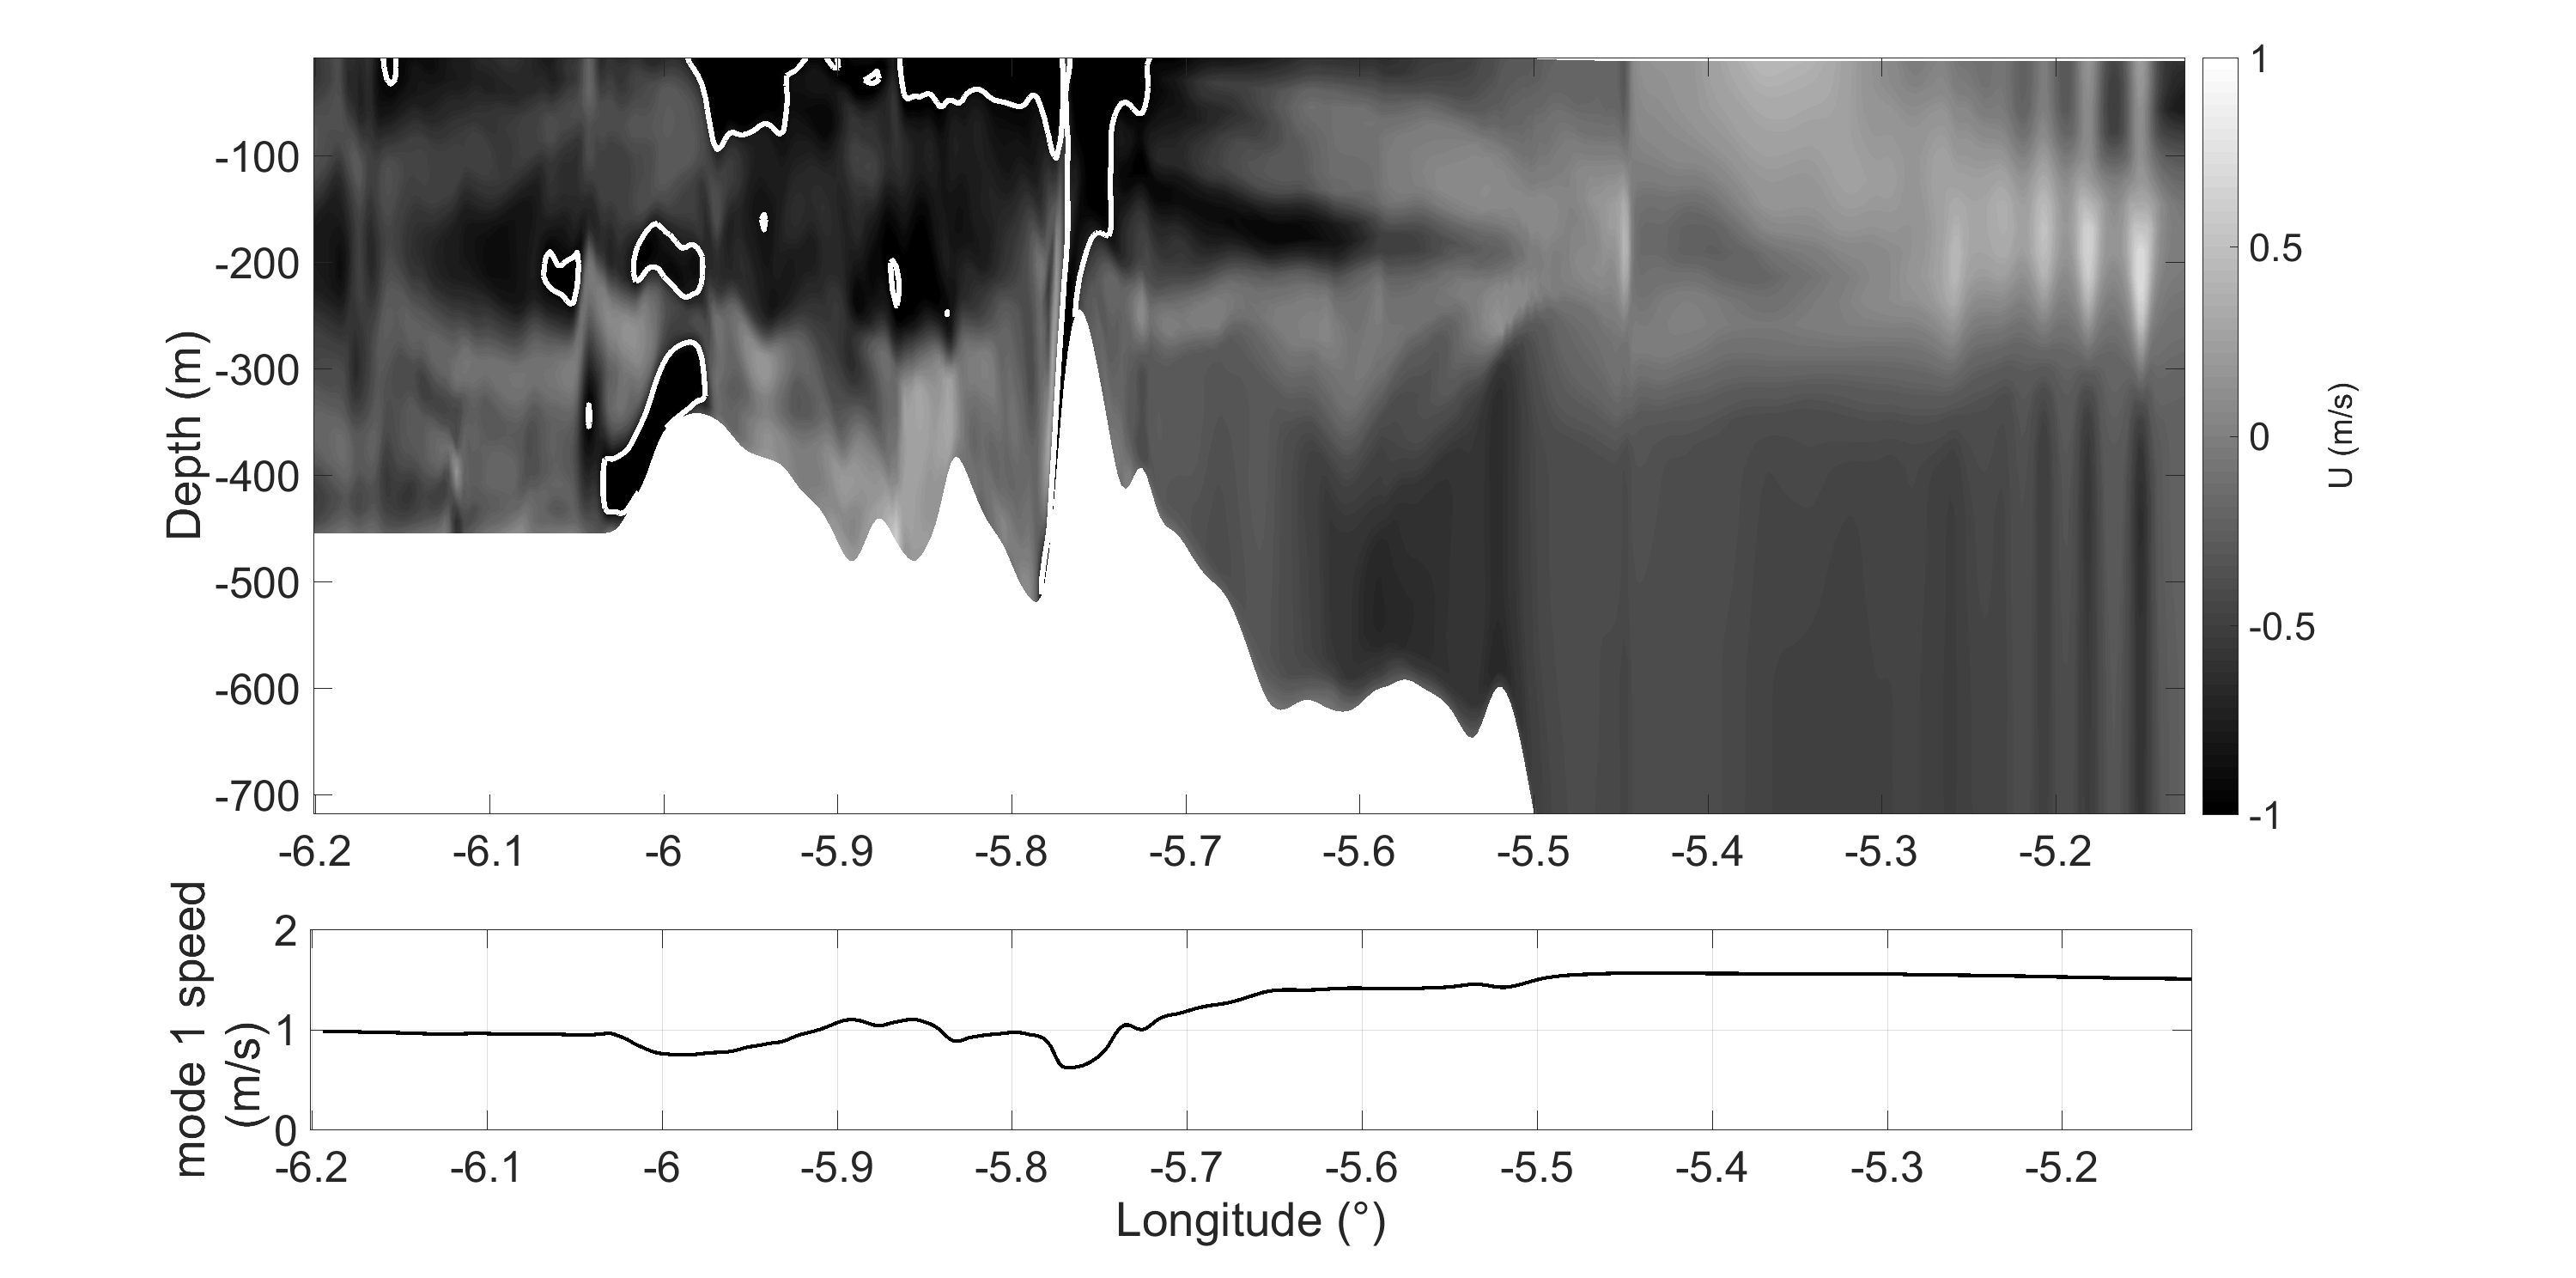
\includegraphics[width=1\linewidth]{./papier2D/comp_fn_strat.png}
\caption{Top panel : field of longitudinal velocity ($u (x,z)$) at $t = 8.5\ T$ with contour of mode 1 supercritical region (F>1) calculated from a 3T-averaged stratification . Bottom panel : Computed linear speed of mode 1 internal waves ($c^*_1 (x)$) from a 3T-averaged stratification in configuration \textbf{SimRef}.}
\label{fig_annexeF}
\end{figure}

 A value $N (x)$ is computed for the water column at each horizontal point of the subsection from a 3T averaged stratification in \textbf{SimRef}. The propagation speed for mode 1 linear waves ($c^*_1 (x)$) is then computed as $c^*_1 (x) =\omega / k_1 (x)$ with $\omega$ the pulsation of the M2-tidal component and $k_1 (x)$ from (\ref{eqK}). This value is indicated in the lower panel of figure \ref{fig_annexeF}, then compared to the field $u(x,z)$ of longitudinal velocity at t=8.5 T plotted in the upper panel. In the upper panel is also highlighted the areas where $u(x,z) > c^*_1 (x)$, hence where the Froude number $F_1$ is superior to 1. The flow inside those contours is called supercritical.
%$N$ can be calculated either from the instantaneous stratification or from a representative one. In figure \ref{fig_annexeF}, the computing of $N$ has been realized either from the field of relative density at t=8.5 T or from a 3T averaged stratification in \textbf{SimRef}. The propagation speed for mode 1 linear waves ($c^*_1$) is then computed and compared to the field of longitudinal velocity at t=8.5 T. 

%There is little difference between the two resulting mapping of supercritical flow. The positions of hydraulic controls at the sills is respected. Only the extent of the areas of F>1 is slightly lesser when based on instantaneous stratification.\color{red}Retirer cette phrase? ou la comparaison tout court...\color{black} As such, we chose to compute Froude numbers from averaged stratification in the present work.

%\color{red}Here we chose to calculate $N$ from the 3T averaged stratification in \textbf{SimRef} visible in figure \ref{fig_fn_ref}.\color{black}
%%%%%%% Biblio

%\newpage
%\nocite{Baines1995}
%\nocite{BS84}
%\nocite{FA1988}
%\nocite{FA1986}
%\nocite{Garett90}
%\nocite{Vazquez2006}
%\nocite{SG2011}
%%\nocite{Sannino2014}
%\nocite{Naranjo2014}
%\nocite{Sannino2009}
%\nocite{Sannino2009b}
%\nocite{Brandt1996}
%\nocite{Sannino2004}
%\nocite{S2005}
%\nocite{Izquierdo2001}
%\nocite{Auclair2018}
%\nocite{SN2015}
%\nocite{CW90}
%\nocite{Beth79}
%\nocite{Bray95}
%\nocite{Sannino2002}
%\nocite{FA1988}
%\nocite{Bormans1989}
%\nocite{Vlasenko2009}
%\nocite{Bryden94}
%\nocite{SG2008}
%\nocite{Wesson94}
%\nocite{Dossmann2012}
%\nocite{Grinstein2007}
%\nocite{Bruno2002}
%\nocite{tpxo8}
%\nocite{alpers85}
%\nocite{Debreu2012}

%%\begin{multicols}{2}
%\bibliographystyle{plain}
%\bibliography{./papier2D/biblio_gib}
%%\end{multicols}

